% Options for packages loaded elsewhere
\PassOptionsToPackage{unicode}{hyperref}
\PassOptionsToPackage{hyphens}{url}
%
\documentclass[
]{book}
\usepackage{lmodern}
\usepackage{amssymb,amsmath}
\usepackage{ifxetex,ifluatex}
\ifnum 0\ifxetex 1\fi\ifluatex 1\fi=0 % if pdftex
  \usepackage[T1]{fontenc}
  \usepackage[utf8]{inputenc}
  \usepackage{textcomp} % provide euro and other symbols
\else % if luatex or xetex
  \usepackage{unicode-math}
  \defaultfontfeatures{Scale=MatchLowercase}
  \defaultfontfeatures[\rmfamily]{Ligatures=TeX,Scale=1}
\fi
% Use upquote if available, for straight quotes in verbatim environments
\IfFileExists{upquote.sty}{\usepackage{upquote}}{}
\IfFileExists{microtype.sty}{% use microtype if available
  \usepackage[]{microtype}
  \UseMicrotypeSet[protrusion]{basicmath} % disable protrusion for tt fonts
}{}
\makeatletter
\@ifundefined{KOMAClassName}{% if non-KOMA class
  \IfFileExists{parskip.sty}{%
    \usepackage{parskip}
  }{% else
    \setlength{\parindent}{0pt}
    \setlength{\parskip}{6pt plus 2pt minus 1pt}}
}{% if KOMA class
  \KOMAoptions{parskip=half}}
\makeatother
\usepackage{xcolor}
\IfFileExists{xurl.sty}{\usepackage{xurl}}{} % add URL line breaks if available
\IfFileExists{bookmark.sty}{\usepackage{bookmark}}{\usepackage{hyperref}}
\hypersetup{
  pdftitle={Comprehensive agriculture guide},
  pdfauthor={Deependra Dhakal, Samita Paudel},
  hidelinks,
  pdfcreator={LaTeX via pandoc}}
\urlstyle{same} % disable monospaced font for URLs
\usepackage{longtable,booktabs}
% Correct order of tables after \paragraph or \subparagraph
\usepackage{etoolbox}
\makeatletter
\patchcmd\longtable{\par}{\if@noskipsec\mbox{}\fi\par}{}{}
\makeatother
% Allow footnotes in longtable head/foot
\IfFileExists{footnotehyper.sty}{\usepackage{footnotehyper}}{\usepackage{footnote}}
\makesavenoteenv{longtable}
\usepackage{graphicx}
\makeatletter
\def\maxwidth{\ifdim\Gin@nat@width>\linewidth\linewidth\else\Gin@nat@width\fi}
\def\maxheight{\ifdim\Gin@nat@height>\textheight\textheight\else\Gin@nat@height\fi}
\makeatother
% Scale images if necessary, so that they will not overflow the page
% margins by default, and it is still possible to overwrite the defaults
% using explicit options in \includegraphics[width, height, ...]{}
\setkeys{Gin}{width=\maxwidth,height=\maxheight,keepaspectratio}
% Set default figure placement to htbp
\makeatletter
\def\fps@figure{htbp}
\makeatother
\setlength{\emergencystretch}{3em} % prevent overfull lines
\providecommand{\tightlist}{%
  \setlength{\itemsep}{0pt}\setlength{\parskip}{0pt}}
\setcounter{secnumdepth}{5}
\usepackage{booktabs}

\usepackage{geometry} % for custom layout of book and landscape geometry support
\usepackage{amsthm}
\makeatletter
\def\thm@space@setup{%
  \thm@preskip=8pt plus 2pt minus 4pt
  \thm@postskip=\thm@preskip
}
\makeatother

\usepackage{longtable}
\usepackage{booktabs}
\usepackage{dcolumn}
\usepackage{tabularx}
\usepackage{array}
\usepackage{multirow}
% \usepackage[table]{xcolor}
\usepackage{wrapfig}
\usepackage{float}
\usepackage{colortbl}
\usepackage{pdflscape}
\usepackage{tabu}
\usepackage{threeparttable}
\usepackage[normalem]{ulem}
\usepackage{rotating}
\newcommand{\blandscape}{\begin{landscape}}
\newcommand{\elandscape}{\end{landscape}}
\usepackage[format=hang,labelfont=bf,margin=0.5cm,justification=centering]{caption}
% \usepackage{exam} % this and exam.sty cause error
\usepackage{pdfpages}

% \usepackage{subcaption} % doesn't work with tinytex in windows
% \newcommand{\subfloat}[2][need a sub-caption]{\subcaptionbox{#1}{#2}}

% simple fix for exam class features of questions and solution
\usepackage{enumitem}

\newlist{questions}{enumerate}{3}
\setlist[questions]{label=\arabic*.}
\newcommand{\question}{\item}

\newenvironment{solution}{ {\bfseries Solution}:}{}
\usepackage[]{natbib}
\bibliographystyle{apalike}

\title{Comprehensive agriculture guide}
\author{Deependra Dhakal, Samita Paudel}
\date{November, 2019}

\begin{document}
\maketitle

{
\setcounter{tocdepth}{1}
\tableofcontents
}
\hypertarget{introduction}{%
\chapter{Introduction}\label{introduction}}

This is a reference manual for self purpose only.

\hypertarget{general-agriculture}{%
\chapter{General agriculture}\label{general-agriculture}}

\hypertarget{nepal-agriculture-and-geography}{%
\section{Nepal agriculture and geography}\label{nepal-agriculture-and-geography}}

\textbf{Ecological regions}
- Himalayan region: 35\%
- Hilly region: 41.67\%
- Terai region: 23.11\%

\textbf{Agricultural land}

\begin{itemize}
\tightlist
\item
  Cultivated land: 3091000 ha (21\%)
\item
  Cultivated land uncultivated: 1030 (6.99\%)
\item
  Jungle and shrubs: 5828 (39.597\%); Shrub alone: 1560
\item
  Pasture land: 1766000 (11.99\%)
\item
  Total Jungle = Shrub + Pasture
\end{itemize}

\textbf{GDP of Agriculture and releated sector/subsectors}

\begin{table}

\caption{\label{tab:unnamed-chunk-2}Percentage contribution of different sector and subsectors to total national GDP}
\centering
\begin{tabular}[t]{lrrr}
\toprule
sector & fy\_2074-75 & fy\_2073-74 & fy\_2072-73\\
\midrule
Agriculture and forestry & 27.10 & 28.25 & 31.08\\
Fishery & 0.49 & 0.51 & 0.53\\
Non-agriculture & 72.41 & 71.24 & 68.39\\
\bottomrule
\end{tabular}
\end{table}

\textbf{Agricultural growth rates}

\begin{verbatim}
## # A tibble: 3 x 2
##    Year `Growth rate (%)`
##   <dbl>             <dbl>
## 1  28.4              0.01
## 2  28.0              5.14
## 3  27.7              2.72
\end{verbatim}

\hypertarget{population-census-2068}{%
\section{Population census, 2068}\label{population-census-2068}}

\begin{verbatim}
## # A tibble: 38 x 1
##    Indicator
##    <list>   
##  1 <chr [1]>
##  2 <formula>
##  3 <chr [1]>
##  4 <chr [1]>
##  5 <dbl [1]>
##  6 <chr [1]>
##  7 <chr [1]>
##  8 <dbl [1]>
##  9 <chr [1]>
## 10 <chr [1]>
## # ... with 28 more rows
\end{verbatim}

\hypertarget{kishan-call-center}{%
\section{Kishan call center}\label{kishan-call-center}}

\begin{itemize}
\tightlist
\item
  Phone number: 1660-5652-999
\item
  Active hours: 10 AM - 4:30 PM
\end{itemize}

\hypertarget{development-of-cooperatives-in-nepal}{%
\section{Development of cooperatives in Nepal}\label{development-of-cooperatives-in-nepal}}

\begin{itemize}
\item
  Traditionally, custom of \emph{Parma}, \emph{Mankakhal}, \emph{Dharmabhakari}, \emph{Dhikuri}/ \emph{Dhukuti} were on place very early.
\item
  In 2010, Cooperative development department was established.
\item
  In 2013, government implemented executive guidelines.
\item
  In 2016, Cooperative organization act came into force.
\item
  In 2018, Cooperative organization regulations came into force.
\item
  In 2019, Cooperative training center was established.
\item
  In 2020, Cooperative bank was established.
\item
  In 2024, ``Village return campaign'' was initiated under cooperative program.
\item
  In 2027, Agriculture development bank started managing cooperative organizations.
\item
  In 2033, ``Sajha'' program was implemented in 30 districts establishing multipurpose cooperatives in VDCs.
\item
  In 2035, Agriculture development bank handed over the managerial responsibility of cooperatives to management board.
\item
  In 2041, Cooperative (``Sajha'') organization act came into force.
\item
  In 2048, National cooperative development board was set up.
\item
  In 2048, Cooperative act came into force (new)
\item
  In 2049, National Cooperative Association was established.
\item
  In 2069, Ministry of cooperative and poverty alleviation was formed.
\item
  Cooperative campaign was first initiated when implementing first five year plan (In 2013), wherein Rapti Dunn Project was launched and 378 cooperative organizations were established in the course.
\end{itemize}

Importance of cooperatives

\begin{itemize}
\item
  Poverty alleviation
\item
  Social and economic support to low income households
\item
  Combines efforts of small producers and consumers and leads them to a larger scale commercial operation
\item
  Reduces transaction cost, when compared to individual efforts
\item
  Reduces chances of suppression and exploitation by large scale acting merchants
\item
  Effective utilization of available resources and supplies
\item
  Empowerment of local community
\item
  Qualitative development of labor
\item
  Improves bargaining power
\item
  Has a bigger role in operationizing in market demand and supply forces
\item
  Members have ownership in rural development
\item
  Promotion of community welfare
\item
  Community development based on justice and equality
\item
  Produce can have more accessible market
\item
  Quality service could be delivered
\item
  Effective mobilization of consumable goods
\item
  Support in national economy
\item
  10th five year plan focused on emphasized agriculture based commerce and industries, cooperative farming, cooperative based agriculture input supply, and cooperative based small farmer irrigation project implementation, dairy collection and supply and other cooperative based approach to community development.
\item
  The plan promoted active participation of cooperative groups and private sectors for the efforts.
\item
  National agriculture policy, 2061 has prioritized cooperative based agriculture industries and commerce promotion, farmer group cooperative formation and agriculture wholesale market and haat bazzar established and management via cooperatives.
\item
  To legalize a cooperative organization establishment, it should be registered:

  \begin{itemize}
  \tightlist
  \item
    Under Organization act in District Administration Office, or
  \item
    According to Cooperative act and regulations under Cooperative Division Office.
  \end{itemize}
\end{itemize}

\hypertarget{budget-speech-2076-77-bs}{%
\section{Budget speech, 2076-77 BS}\label{budget-speech-2076-77-bs}}

Total budget announced was Rs 1.53 trillion for fiscal year 2019/20 (76/77). Economic growth rate was set at 7\% as target. The budget focuses on social justice, increment of export to reduce trade deficit and increase in general productivity.

NRs 130 billion is to be distributed from revenue between provincial and local levels. Education will be freed upto secondary level. In terms of literacy, 70 districts will be designated the status of fully literate districts. To that end, NRs 2 billion will be appropriated for colorful textbooks for primary level. Day meals for 2.2 million school children will be provisioned and sanitary pads will be free for female students attending public schools.

Over 10 billion was allocated for Madan Bhandari science and technology university. It is also stated that science and technology laboratory will be established in each province.

NRs 6 billion will be allocated for free insurance in all districts.

Health grants will be increased for treatment of 8 types of severe illnesses. Likewise, NRs 2.2 billion is appropriated for new-mothers travel expenses. 52000 female community health volunteers will be provided Rs 3000 annual allowance. NRs 5 billion is dedicated to establish health service providing facilities at local levels. Similarly, Rs 400 milion is allocated for Ramraja Prasad Singh Hospital in Rajbiraj. Rs 400 million appropriated for betterment of Bir Hospital.

Addressing issue of public health, smoking and drinking will be banned in public places. 92\% of the population will be provided full access to drinking water in coming fiscal year. NRs 7 billion is allocated for completion of Melamchi drinking water project. Over 43 billion NRs is allocated for drinking water and hygiene.

Social security allowance to pregnant women and elderly senior citizens allowance sees an increment of Rs 1000 (increased from Rs 2000 to 3000). There have been betterment of employment schemes for the peoples with disabilities.

Coming fiscal year to marked as youth mobilization year. Youth scientists conference to be held in the coming year.

In agriculture, grants will be provided for purchase of agricultural products and technology. Schemes for achieving self sufficiency in dairy, poultry and fresh vegetables will be prepared and implemented. Grants will be provided for fertilizer input purchase. Organic farming wil be encouraged. With the dubling of fruit cultivation in next 5 years, food quality labs will also be set in every province. Rs 500 million is appropriated for community farming. Rs 34 billion is allocated for agriculture.

A budget of 23.6 billion is allocated for irrigation programmes. 960 million allocated for irrigation programmes in Terai. Sunkoshi Marine to be developed as a national pride project, with 2.05 billion NRs allocated for program initiation. NRs 5.6 billion is allocated for construction of dams.

Next fiscal year will be marked as tree plantation year. Security to be beefed up in forest areas. Newer programs/practices to be launced in livestock management. Rs 1 billion is dedicated for `Rastrapati Chure Programme'.

Under land management, a revised land management act will be introduced for sustainable utilization of land. Encroached public lands will be brought under government management within next fiscal year. Online issuance of land ownership certificate will have been started by next two years.

Tourism sector will be prioritized, with stress on infrastructure development of main tourist areas. Trail connecting Darchula to taplejung to be developed. Operation of cable cars will be encouraged in mountainous regions.

Government officials will be mandated to only gift homemade (domestic) products as and when needed.

Private and cooperative sector to be encouraged for production of necessary commodities. Local cement and wire frames to be encouraged in construction. To be self sufficient in production of at least 2 dozen products.
- Hetauda and Udayapur cement factories to be made more efficient
- Local products will be promoted in construction inputs
- Import of luxury goods and health unfriendly products to be discouraged
- Economic zone to be established in Kavre and Nuwakot. 50\% concession to Nepali textile industry on electricity.

Infrastructure development at trade transit points in the north. Business with third countries to begin via Chinese port. Completion of pending works on pipeline by the next year to facilitate import of petroleum products.

In energy, at least two big hydropower projects will be embarked on in all seven provinces. NRs 13 billion is allocated for Budigandaki, 2.02 for Budhiganga-Tamor project to be a national pride project. Province 2, Karnali province and Sudurpaschim province to have full access to electricity. Rs. 4.5 billion allocated for rural electrification. Waste-to-energy programmes will be encouraged.

Rs 163 billion is appropriated for railway and waterways. Digital payment system will be installed in public transport. 1.5 billion for transport management. Electric buses to be introduced in ``major'' cities. NEA to install charging stations. Additional budget is allocated for development of Narayani and Koshi waterways.

Under urban development, feasibility study will be conducted for development of mega-city and smart city. 530 million allocated to replace thatched roofs of 20000 houses. 4.3 billion for construction of 30000 houses under housing project.

Convention center with a capacity to accomodate 3000 people to be constructed in the valley, this year. City halls to be constructed in local levels. Compulsory footpath, underground cable management. Rs 47.7 billion allocated for housing and urban development. MP's constituency budget (MP fund) increased to Rs 60 million. 1 billion for Dharahara reconstruction (to be completed within the next two years). 141 billion appropriated for reconstruction. Rs 9 billion isolated for infrastructural development in each electoral constituency.

Online visa services will be furnished for foreign nationals. National Defence University to be established. 18-20\% (non-gazetted and gazetted) increment in salaries of public service personnel. National knowledge centre to be established at Khumaltar, Tribhuvan International Airport to be upgraded to a boutique airport. Gautam Buddha International airport to come into operation next year. Contractors to be held responsible for the upkeep of their projects for years after completion.

VAT and other taxes to be made more effective through improved taxation system VAT rates to stay intact changes in customs rate. Import reliance will be significantly reduced.

The budget size is 1.53 trillion, recurrent budget is 957.1 billion, capital expenditure is 408.59 billion and financing 167.5 billion.

\hypertarget{food-security}{%
\section{Food security}\label{food-security}}

For a more fundamental discussion of food security topic, refer to \href{https://github.com/DeependraD/life_science_presentations/raw/master/food_security.pdf}{lecture handout}, in link to life science presentations.

FAO defined food security in 1996 A.D. In 1996, convention held in Rome approved seven points of food soverignty. Nepal has been a member of FAO since 2007 BS (1950 AD).

McMichael's projection:
- 2 billion people suffer hidden hunger
- 1.5 billion people suffer over nutrition related problems

Since 1981 (2038 BS), FAO started celebrating World Food Day on October 16th. In Nepal, 34th World Food Day was celebrated in 2014 with the slogan: ``Feeding the world, caring for the earth''.

According to FAO's projection, 52\% of the population in South Asia are dependent on Agriculture while agriculture contributes 22\% to the total GDP in the region.

Pillars of food security:

\begin{enumerate}
\def\labelenumi{\arabic{enumi}.}
\tightlist
\item
  Food availability
\item
  Food access
\end{enumerate}

\begin{itemize}
\tightlist
\item
  Nepal's poverty rate in 2001/2002 AD: 30\%
\item
  Nepal's poverty rate in 2010 AD: 26\%
\item
  Nepal's poverty rate at the end of 12th plan: 23.8\%
\end{itemize}

\begin{enumerate}
\def\labelenumi{\arabic{enumi}.}
\setcounter{enumi}{2}
\tightlist
\item
  Food utilization
\end{enumerate}

\begin{itemize}
\tightlist
\item
  Per person per day recommendation by WHO: 250 ml milk (91 ltr per year)
\item
  Nepal's aim for per day milk consumption: 156 ml (57 ltr per year)
\item
  Nepal's aim for per year meat consumption: 14 kg
\item
  Nepal's aim for per year egg consumption: 48
\item
  30\% of total daily protein requirement should be met by animal sources.
\end{itemize}

\begin{enumerate}
\def\labelenumi{\arabic{enumi}.}
\setcounter{enumi}{3}
\tightlist
\item
  Food stability
\end{enumerate}

\begin{itemize}
\tightlist
\item
  In 2011 AD, Nepal ranked 157th among 187 nations in HDI
\item
  In 2014 AD, Nepal ranked 145th in HDI
\item
  Poverty rate at village/rural areas: 27\% (Survey, 2012)
\item
  Poverty rate at cities: 15\% (Survey, 2012)
\item
  Monthly poverty:

  \begin{itemize}
  \tightlist
  \item
    Maximum at Chaitra-Baisakh
  \item
    Minimum at Mangsir-Poush
  \end{itemize}
\end{itemize}

State of food security in Nepal:

\begin{itemize}
\tightlist
\item
  Untill 2042 BS (1985), production was twice that satisfied the population's need.
\item
  Upto 2047 BS, food insufficieny was absent.
\item
  Currently 40 districts are declared food minimum and more than 27 districts of high hill and mountain districts are food insecure.
\item
  Calorie deficiency is prevalent in 41\% of population.
\item
  In 19 districts of Midwestern Development Region and Eastern Development Region, food security project is launched.
\item
  46\% of the total cultivated area is under rice.
\item
  Of the total food production, contribution of respective crops are:

  \begin{itemize}
  \tightlist
  \item
    Rice: 56\%
  \item
    Maize: 24\%
  \item
    Wheat: 17\%
  \item
    Millet: 3.6\%
  \item
    Barley: 0.29\%
  \end{itemize}
\end{itemize}

\hypertarget{nepal-agriculture-research-council}{%
\section{Nepal agriculture research council}\label{nepal-agriculture-research-council}}

\begin{itemize}
\tightlist
\item
  Has following organizational structure:

  \begin{itemize}
  \tightlist
  \item
    Executive director
  \item
    Director, Planning and cooperation
  \item
    Director, Crop and horticulture research
  \item
    Director, Livestock and fisheries research
  \item
    Director, Employee administration
  \item
    Director, Economic adminsistration
  \item
    Head, Planning commission
  \item
    Communication, publication and inventory commission
  \item
    Socio-economic and agricultural research policy commission
  \item
    External research directorate
  \item
    Agriculture environment directorate
  \end{itemize}
\item
  Programs under Agronomic and horticultural crop research programs

  \begin{itemize}
  \tightlist
  \item
    Rice crop research program, Baniniya, Dhanusha
  \item
    Maize research program, Rampur, Chitwan
  \item
    Wheat crop research program, Bhairahawa, Rupandehi
  \item
    Legume crop research program, Nepalgunj
  \item
    Oil crop research program, Nawalpur, Sarlahi
  \item
    Hilly crop research program, Kavre, Dolakha
  \item
    Sugarcane research program, Jitpur, Bara
  \item
    Potato research program, Khumaltar
  \item
    Ginger research program, Salyan
  \item
    Orange variety research program, Dhankuta
  \item
    Jute crop research program, Itahari, Sunsari
  \item
    National commercial agriculture research program, Pakhribas, Dhankuta
  \end{itemize}
\item
  Divisions situated in Khumaltar

  \begin{itemize}
  \tightlist
  \item
    Crop science division
  \item
    Crop disease science division
  \item
    Entomology science division
  \item
    Soil science division
  \item
    Agri-engineering division
  \item
    Agri-botany division
  \item
    Horticulture research division
  \item
    Food research division
  \item
    Biotechnology division
  \item
    Commercial crop division
  \item
    Seed science and technology research division
  \end{itemize}
\end{itemize}

Regional agriculture research centres and programs

\begin{enumerate}
\def\labelenumi{\arabic{enumi}.}
\tightlist
\item
  Regional agriculture research centre, Nepalgunj
\end{enumerate}

\begin{itemize}
\tightlist
\item
  ARC, Surkhet
\item
  ARC, Doti
\item
  ARC, Jumla, Bijayanagar
\item
  ARC, Jumla, Rajikot
\item
  ARC, Dolakha
\end{itemize}

\begin{enumerate}
\def\labelenumi{\arabic{enumi}.}
\setcounter{enumi}{1}
\tightlist
\item
  Regional agriculture research centre, Lumle
\end{enumerate}

\begin{itemize}
\tightlist
\item
  ARC, Baidam, Pokhara \(\rightarrow\) Aquaculture
\item
  ARC, Begnas, Pokhara \(\rightarrow\) Aquaculture
\item
  ARC, Malepatan, Pokhara \(\rightarrow\) Horticulture
\item
  ARC, Bandipur, Tanahun \(\rightarrow\) Goat
\end{itemize}

\begin{enumerate}
\def\labelenumi{\arabic{enumi}.}
\setcounter{enumi}{2}
\tightlist
\item
  Regional agriculture research centre, Parwanipur
\end{enumerate}

\begin{itemize}
\tightlist
\item
  ARC, Rasuwa \(\rightarrow\) Pasture
\item
  ARC, Ranighat, Birgung, Parsa \(\rightarrow\) Agri-machinery
\item
  ARC, Trishuli \(\rightarrow\) Acquaculture
\item
  ARC, Belachhapi, Dhanusha \(\rightarrow\) Tobaccoo
\end{itemize}

\begin{enumerate}
\def\labelenumi{\arabic{enumi}.}
\setcounter{enumi}{3}
\tightlist
\item
  Regional agriculture research centre, Tarahara
\end{enumerate}

\begin{itemize}
\tightlist
\item
  Pakhribas, Dhankuta
\item
  Tarahara \(\rightarrow\) Aquaculture
\end{itemize}

\hypertarget{ads}{%
\section{ADS}\label{ads}}

\begin{itemize}
\tightlist
\item
  MoAD, ADB, Rastriya Kishan Sanjal etc. including 12 development cooperatives (technical team) were involved in preparation of the strategy.
\item
  Vision (7 sub heads):

  \begin{itemize}
  \tightlist
  \item
    Self reliance
  \item
    Sustainablity
  \item
    Competition
  \item
    Inclusive
  \item
    Growth
  \item
    Livelihood
  \item
    Food and nutrition security
  \end{itemize}
\item
  There are 16 indicators ??
\end{itemize}

\hypertarget{national-farmers-commission}{%
\section{National Farmers Commission}\label{national-farmers-commission}}

\begin{itemize}
\tightlist
\item
  Chariman: Chitra Bahadur Shrestha
\item
  Members: 7 total
\item
  2073/10/06: National Farmers' Commission organization directives
\item
  Has central office in Hariharbhawan, Lalitpur
\end{itemize}

\hypertarget{prime-minister-agriculture-modernization-project}{%
\section{Prime minister agriculture modernization project}\label{prime-minister-agriculture-modernization-project}}

Initiation, project details \ldots{}

\hypertarget{zones-and-superzones}{%
\subsection{Zones and superzones}\label{zones-and-superzones}}

\hypertarget{crop-and-livestock-insurance}{%
\section{Crop and livestock insurance}\label{crop-and-livestock-insurance}}

\hypertarget{one-village-one-commodity-odop}{%
\section{One village one commodity (ODOP)}\label{one-village-one-commodity-odop}}

\hypertarget{one-district-one-commodity}{%
\section{One district one commodity}\label{one-district-one-commodity}}

\hypertarget{impacts-of-climate-change}{%
\section{Impacts of climate change}\label{impacts-of-climate-change}}

What are the impacts of climate change ? Discuss on detail about the initiative taken by Nepal Government in tackling the impacts of climate change.

Climate change is now affecting every country in every continent. It is disrupting national economies and affecting lives, of individuals, communities and countries today and is likely to do so in the ensuing future. Weather pattern are changing, snowline are melting due to global warming and sea level are rising.

\textbf{Negative impacts}

\begin{enumerate}
\def\labelenumi{\arabic{enumi}.}
\tightlist
\item
  Numerous mountains are seeing accelerated the melting of snow due to global warming.
\item
  Changes in monsoon patterns, such as erratic rainfall with alternate drought periods are the serious impacts of climate change in Nepal which hampers the agricultural production. The changes in monsoon pattern in Nepal greatly exacerbate the situation of poverty and food insecurity in the country.
\item
  Flood, landslides, forest fires, snow melt are the disasters that occur as a result of climate change without any prewarning and causes heavy loss.
\item
  High hills and mountains are more vulnerable to climate change compared to terai, thus climate change make large scale economic and ecolgical disruption in upper latitudes.
\item
  Loss of plant and animal biodiversity.
\item
  Increase in number of insects, pest and diseases and sporadic outbreaks becoming much frequent.
\end{enumerate}

The positive impact of global warming, a characteristic feature of climate change, is that the crops that could in the past be only growth in certain low altitudes, requiring prolonged exposure to heat can now be growth in higher regions such as Manang and Mustang districts of Nepal. The is evidently due to increase average temperature of the region, thus allowing the crop to perform well. However, as noted earlier, there are more prominent negative impacts than the benifits we can derive from the climate change.

Nepal became signatory of UN Framework Convention on Climate Change (UNFCC) in 1994. Ever since then the issue of climate change has been routinely incorporated into policy and strategic frameworks by Government of Nepal. Following policies and strategies are currently in place to help mitigate the impacts of climate change in Nepal:

\begin{enumerate}
\def\labelenumi{\arabic{enumi}.}
\tightlist
\item
  Constitutional approach
\end{enumerate}

Article 30(1) of the constitution of Nepal guarantees a ``clean environment'' as fundamental right and elaborates that ``every citizen shall have the right to live in a clean and healthy environment.'' Article 30(2) of the constitution also encourages the state to formulate necessary legal framework to balance environment and development.

\begin{enumerate}
\def\labelenumi{\arabic{enumi}.}
\setcounter{enumi}{1}
\tightlist
\item
  Approaches in periodic plans
\item
  Climate change policy, 2067 (2011)
\item
  National climate change policy, 2076 (2019)
\item
  National adaptation plan of action (NAPA, 2010)
\item
  Framework for local adaptation plan for action (LAPA, 2011)
\end{enumerate}

\hypertarget{highlights-of-nccp-2076}{%
\subsection{Highlights of NCCP, 2076}\label{highlights-of-nccp-2076}}

Reasons for Nepal's vulnerability to climate change are Topographical fragility, fragile geological structure, sensitive ecosystems and diversity of climate and micro-climate zones prevalence in Nepal. Additionally, poverty, illiteracy, social disparity and high dependence of communities on natural resources for livelihood.

\begin{itemize}
\tightlist
\item
  Nepal National Red Strategy implemented to check greenhouse gases emmission from deforestation and forest destruction.
\item
  Provision of climate change coordination committee in Chairmanship of Prime minister.
\item
  Establishment of Climate change management section under Ministry of Forest and Environment as focal point for implementation of international treaty.
\item
  Provision of Climate budget code by National planning commission.
\item
  Alternative energy promotion center has established climate and carbon unit for executing Clean Development Mechanism (CDM) related activities.
\end{itemize}

\textbf{Goal}

To contribute to socio-economic prosperity of the nation by building a climate resilient society.

\textbf{Objectives}

\begin{enumerate}
\def\labelenumi{\alph{enumi}.}
\tightlist
\item
  To enhance climate change adaptation capacity of persons, families, groups and communities vulnerable to, and at risk of, climate change;
\item
  To build resilience of ecosystems that are at risk of adverse impacts of climate change;
\item
  To promote green economy by adopting the concept of low carbon emmission development;
\item
  To mobilize national and international financial resources for climate change mitigation and adaptation in just manner;
\item
  To conduct research, make effective technology development and information service delivery related to climate change;
\item
  To mainstream or integrate climate change issues into policies, strategies, plans and programs at all levels of State and sectoral areas;
\item
  To mainstream gender equality and social inclusion (GESI) into climate change mitigation and adaptation programs.
\end{enumerate}

\textbf{Policies} (Sectoral policy, strategies and working policies)

\begin{enumerate}
\def\labelenumi{\arabic{enumi}.}
\tightlist
\item
  Agriculture and food security
\item
  Forest, biodiversity and watershed conservation
\item
  Water resources and energy
\item
  Rural and urban habitats
\item
  Industry, transport and physical infrastructure
\item
  Tourism and natural and cultural heritage
\item
  Health and drinking water and sanitation
\item
  Disaster risk reduction and management
\item
  Gender equality and social inclusion, livelihoods and good governance
\item
  Awareness raising and capacity development
\item
  Research, technology development and expansion
\item
  Climate finance management
\end{enumerate}

Policy number 9-12 are inter-thematic areas.

\hypertarget{horticulture}{%
\chapter{Horticulture}\label{horticulture}}

\hypertarget{plant-growth-hormones}{%
\section{Plant growth hormones}\label{plant-growth-hormones}}

\hypertarget{abscissic-acid}{%
\subsection{Abscissic acid}\label{abscissic-acid}}

Physiological effects of ABA

\begin{enumerate}
\def\labelenumi{\arabic{enumi}.}
\tightlist
\item
  Induction of dormancy of plant organs
\item
  Water balance of plants
\end{enumerate}

\begin{itemize}
\tightlist
\item
  Additionally, ABA plays roles as antagonist of other phytohormones.
\item
  Stratification causes reduction in ABA content and so promotes germination (eg. walnut)
\item
  Inhibition of seed germination by ABA may be reversed by GA application.
\item
  ABA induces formation of storage proteins in seed.
\item
  Bud dormancy is frequently correlated with increase in ABA concentration.
\item
  During vernalization, however, ABA content falls.
\item
  ABA regulates water balance (causes stomatal closure and increase in root growth and hydraulic conductivity rise in water deficit).
\end{itemize}

\hypertarget{growth-stages-of-cabbage-9-distinguishible}{%
\section{Growth stages of cabbage (9 distinguishible)}\label{growth-stages-of-cabbage-9-distinguishible}}

\begin{enumerate}
\def\labelenumi{\arabic{enumi}.}
\tightlist
\item
  Cotyledons: No true leaves present
\item
  Seedling: Upto 5 true leaves
\item
  6-8 true leaf
\item
  9-12 true leaf: Base of stem still visible from above
\item
  Precupping: Approximately 13-19 leaves. By the end of this stage, the base of stem and the bases of all leaves are concealed when plant is viewed from above. The innermost heart leaves are growing in an upright fashion and are visible without moving any of the surrounding leaves.
\item
  Cupping: Approximately 20-26 leaves. The innermost heart leaves, which are still growing in an upright fashion, are concealed by the larger, older leaves surrounding them. All visible leaves will later become the frame leaves (leaves not touching the mature head) of the mature plant.
\item
  Early head formation: Approximately 2.5-4 inch diameter head. The inner heart leaves, now quickly developing as a ball-like structure of overlapping leaves, are concealed by the surrounding larger leaves. These leaves do not press tightly against the developing head and will later unfold to become frame leaves.
\item
  Head fill: Approximately 3-8 inch diameter head. A firm round head is visible within the wrapper leaves (the 4 outer loose leaves that touch the mature head). The head has not yet fully developed and thus, is not of harvestable size.
\item
  Mature: Approximately 6-12 inch diameter head. No new visible leaf production will occur after the head has attained maximum hardness and size. The head is ready for harvest and may split if not harvested in time.
\end{enumerate}

\hypertarget{citrus-cultivation}{%
\section{Citrus cultivation}\label{citrus-cultivation}}

\hypertarget{principal-rootstocks}{%
\subsection{Principal rootstocks}\label{principal-rootstocks}}

Today, five types of rootstock predominate in relatively not cool climates where cold or freezing weather is not probable, especially Florida and southern Europe.

Sour orange rootstock: it is the only rootstock that truly is an orange (the Citrus ? aurantium or bitter orange). It is vigorous and highly drought-resistant.

Poncirus trifoliata: it is a close relative of the Citrus genus, sometimes classified as Citrus trifoliata. It is especially resistant to cold, the tristeza virus, and the fungus Phytophthora parasitica (root rot) and grows well in loam soil. Among its disadvantages are its slow growth-it is the slowest growing rootstock-and its poor resistance to heat and drought. It is primarily used in China, Japan, and areas of California with heavy soils.

Swingle citrumelo: it is tolerant of tristeza virus and Phytophthora parasitica and moderately resistant to salt and freezing. This rootstock selection was hybridized from the Duncan grapefruit (Citrus paradisi Macfadyen) and the Poncirus trifoliata (L.) Raf. by Walter Tennyson Swingle in Eustis, Florida, in 1907. It was released by the US Department of Agriculture to nurserymen in 1974.

Troyer citrange and Carrizo citrange: these reasonably vigorous rootstocks are resistant to Phytophthora parasitica, nematodes, and tristeza virus and show good cold tolerance. They also are highly polyembryonic, so growers can obtain multiple plants from a single seed. Citrange, however, does not do well in clay, calcareous or high-pH soils, and is sensitive to salinity. It is not feasible as rootstock for mandarin scions, as it overgrows them by producing branches of its own in competition with the grafted budwood.{[}3{]} Citranges are hybrids of the Washington navel orange and the Poncirus trifoliata. The original crosses, made in the early 1900s by the U.S. Department of Agriculture with the intention of producing cold tolerant scion varieties, were later identified as suitable for use as rootstocks. The commercial use of these rootstocks began in Australia in the 1960s. The Troyer variety generally is found in California, while the Carrizo variety is used in Florida.

Cleopatra mandarin: it is tolerant of salinity and soil alkalinity and also suitable for shallow soils. It is used primarily in Spain, Australia, and Florida. Dade County, for example, has 85\% calcareous soil, a typical trait of land that has been under water.{[}4{]} The Cleopatra mandarin, originated in India and introduced into Florida from Jamaica in the mid-nineteenth century, has been distributed and tested as a rootstock throughout the world. Nowadays, however, it is considered an inferior rootstock because it is sensitive to many diseases, grows slowly, and is difficult to propagate.

\hypertarget{guava-cultivation}{%
\section{Guava cultivation}\label{guava-cultivation}}

\begin{itemize}
\tightlist
\item
  \emph{Psidium guajava} (Myrtaceae)
\item
  Origin: Tropical america; originated in the warm, lowland tropics
\item
  Contains low energy, low fat and high amounts of vitamin C.
\item
  Commercial trade is smaller in volume compared to other fruits.
\end{itemize}

\hypertarget{morphology-and-botany}{%
\subsection{Morphology and Botany}\label{morphology-and-botany}}

\begin{itemize}
\tightlist
\item
  Photoperiod insensitive
\item
  Can be forced to flower by pruning
\item
  Woody is hardy; resistant to strong winds.
\item
  The rhythmic flushing of vegetative growth and flowering influences when and how pruning is
  carried out.
\item
  Guavas are forced to produce year round, and normally the actively growing shoots are tipped once they become too large. This tipping forces regrowth and new flowers to be induced, to keep production high and constant.
\item
  As soon as the harvest is finished, a peripheral pruning of the canopy is performed, in order to force new shoots that will bear flowers.
\end{itemize}

\hypertarget{climate-and-soil}{%
\subsection{Climate and soil}\label{climate-and-soil}}

\begin{itemize}
\tightlist
\item
  Temperature lower than \(8\ ^\circ C\) is inappropriate for commercial cultivation.
\item
  Moderately tolerant to saline conditions.
\end{itemize}

\hypertarget{varieties}{%
\subsection{Varieties}\label{varieties}}

\begin{itemize}
\tightlist
\item
  Lucknow-49, Allahabad safeda, Seedless
\end{itemize}

\hypertarget{propagation}{%
\subsection{Propagation}\label{propagation}}

\begin{itemize}
\tightlist
\item
  Stem and root cuttings, Air layering and Budding
\item
  Guava trees propagated by grafting have tap roots that provide substantial anchorage.
\item
  Trees propagated by cuttings have weaker root
  systems.
\end{itemize}

\hypertarget{planting-and-orchard-establishment}{%
\subsection{Planting and orchard establishment}\label{planting-and-orchard-establishment}}

\begin{itemize}
\tightlist
\item
  Spacing with fillers: 3.1 x 7.6 (424 trees/ha)
\item
  Permanent spacing: 6.2 x 7.6 (212 trees/ha), or 4.6 x 7.6 (286 trees/ha)
\end{itemize}

\begin{table}

\caption{\label{tab:climac-vs-nonclim}Climacteric and non climacteric fruits commonly cultivated in Nepal}
\centering
\begin{tabular}[t]{ll}
\toprule
climacteric & non\_climacteric\\
\midrule
\rowcolor{gray!6}  Avocado & Litchi\\
Banana & Mangosteen\\
\rowcolor{gray!6}  Guava & Pineapple\\
Mango & Mountain apple (Bayer)\\
\rowcolor{gray!6}  Papaya & \\
\addlinespace
Sapota & \\
\bottomrule
\end{tabular}
\end{table}

\hypertarget{post-harvest}{%
\subsection{Post-harvest}\label{post-harvest}}

\begin{itemize}
\tightlist
\item
  High moisture loss occurs
\item
  No dramatic change in taste during storage at higher temperatures (10-15 \(\ ^o C\))
\end{itemize}

Horticulture development and plans and policies

Q. Government plans and policies have given priority on horticulture. However, the potentiality of fruit sector (an important component of horticulture) has not been exploited properly. In this context, discuss the current problems relating to fruit crop development in Nepal.

A. \(\longrightarrow\) Although the long term Agriculture Perspective Plan fared well with the set target in horticulture sector (along with roads and community forest) during the implementation period of 1995-2015, overall history of horticulture sector is less than satisfying in Nepal.

The total area, productive area, production and productivity of fruits in the Fiscal Year (FY) 2014/15 are 150387 ha, 110802 ha, 992703 mt and 8.96 mt/ha respectively (Table \ref{tab:horticulture-fruits-veg}). Recent data shows that contribution of horticulture sector amounts to 15\% of the Agriculture GDP. Fruit sub-sector contributes 5.24 ??(when) percent in Agricultural GDP. Besides government engaging in active production of fruit seedlings and provisioning gardening tools, many private firms are working on production of quality planting materials.

Out of total area occupied by fruits 57\% are tropical, 26\% are citrus and only 17\% are temperate fruit species. Similarly, total area covered by fruits is 4.79\% of total cultivated area. It was found that the productivity trend is increasing from 2005/06 (9.47mt/ha) to 2011/12 AD (10.17 mt/ha) and decreasing in 2012/13 (9.25 mt/ha) and in 2013/14 (8.77mt/ha). There is huge gap between exported (24812.17 mt) and imported (2,27,00,266 mt) scenario of different fruits which indicates the immense scope of fruit development in Nepal. Out of 470 fruit nurseries 272 were registered and 198 were non registered.

Currently, more than 90\% of the citrus seedlings are annually distributed by private fruit nurseries. Technical support services to the fruit growers are also being provided by government farms in their command areas and to the pocket areas of the targeted districts through the extension service.

\begin{table}

\caption{\label{tab:horticulture-fruits-veg}Status of fruits and vegetable production and area during recent 3 years.}
\centering
\begin{tabular}[t]{llrrr}
\toprule
Description & Component & 2013-14 & 2014-15 & 2015-16\\
\midrule
Fruit & Area & 110086 & 110802 & 110586\\
Fruit & Production & 965044 & 991978 & 976461\\
Vegetable & Area & 254931 & 266937 & 280807\\
Vegetable & Production & 3421035 & 3580084 & 3929034\\
\bottomrule
\end{tabular}
\end{table}

About 3-4 percent of cultivated land is under fruit acreage. This could be observed from the table below showing the annual cultivation trend since 2005-06 AD. There is an increasing trend in area coverage and fruit production but the yield per hectare is low in comparison with other fruit producing countries. The fruit production needs to be increased to meet the increasing demand for domestic consumption and for exports as well. There are some important issues like infrastructure, physical and environmental, agronomic and technical support post harvest losses, problem oriented research and transfer of technology, which need to be addressed to promote fruit development in the country.

There are 45 species belonging to 37 genera of wild edible fruits. Even seasonal fruits harvested from forests can be seen in several local markets. Despite of increasing area and production and huge potential of fruit cultivation in the country, the quantity and value of foreign import of fruits is increasing in recent years due to higher rate of the increasing internal demand in comparison to rate of increasing domestic production and supply. The per capita availability of fruit in the fiscal year 2014/15 was 34 kg/year.

Major problems relating to development of fruit crops in particular, and horticulture sector in general, are as follows:

\begin{enumerate}
\def\labelenumi{\arabic{enumi}.}
\item
  Despite immense potential of hoticultural crops, upto 80\% of the cultivated land in Nepal is used to grow cereal crops. Out of remaining 20\% cultivated land, most of which are located in more northern latitudes, suitability of fruit farming in those lands is fringe. Most are rocky terrains with steep slopes and young soil. In addition, hilly regions of Nepal suffer a major setback on soil moisture management, which is critical for a fruit orchard. Without a proper buffer against hailstorm and snowfall, substantial amounts of fruit drops and wastage have been noted.
\item
  Since a long time past, unavailability of inputs like inorganic fertilizers, progagation materials have hindered progressive farming. Rural farmers are forced to opt for low input management which only give marginal yields and limits the productivity improvement. Furthermore, as fruit crops are given an inferior status relative to cereals, farmhold themselves are negligent about timely provisioning of agricultural inputs for fruit orchard.
\item
  Irrigation management
\item
  Postharvest handling
\item
  Marketing and transport
\item
  APP was based on a narrow viewpoint of technology -- excessively focused on green revolution perspective that is not appropriate for large parts of Nepalese agroecology. Horticulture sector in particular is largely hurt by this conservative view point of technology adoption. This sector has poorly prospered in terms of access to infrastructure and is one of the least industrially benefitting ones. As hills and rural parts of country are infact the major hubs of vegetable and fruit production, policy emphasis on adoption of more capital intensive technology i.e., that which characterizes green revolution, is just a dream chase afterall. On the other hand, Nepal has areas where specialized farming systems, such as organic citrus and apple production system, could flourish. These regions would have sought mostly technical support for quality assurance, policy support for certification, and basic resource support. All of this were lacking in places such as Mustang, Dolpa and Jumla, where organic apple production could have comparative advantage.
\item
  With the diverse agroecology, we have southern terai regions suited for cultivation of tropical fruits while mid-hills and high-hills towards north being suitable for sub-tropical to warm and cold temperate fruit and nut species. Research and development programs are not found to have exerted impact on all agroecologies, mostly that of Far Western Development Region of Nepal.
\item
  There still are several fruit and nut crops that have a greater local demand but are not being integrated into mainstream research and crop development process. Fruit nuts such as chestnut ( \emph{Castanea} spp.), Sapota, Rubus berry are underutilized while some are at best only identified. Thus, in meeting increasing need of human nutrition and feeding urban population, these minor fruits could play an important role.
\end{enumerate}

Policy level and action oriented strategies that have been or could potentially be taken by Government to uplift horticulture sector include improvement in mainly following aspects:

\begin{enumerate}
\def\labelenumi{\arabic{enumi}.}
\item
  The Decentralization strategy of ADS foresees a decentralized structure of Nepalese Agricultural Research, with establishment of new national research institutes (eg, a National Horticultural Research Institute, National Animal Health Research Institute, and National Aquaculture and Fisheries Research Institute), establishment of a National Agricultural Research Fund (NARF) under NARC, and the establishment of research stations in all regions, including the far western region.
\item
  Nutritional aspect of food security has a prominent role of hoticultural crops. Because fruits and vegetables supply the bulk of fiber, minerals and vitamins, meeting nutritional need of growing urban cummunity is possible only through empowering of horticulture sector.
\item
  ADS highlights following key strategies in improvement of fruit sub-sector of horticulture:
\end{enumerate}

\begin{itemize}
\tightlist
\item
  Formulation and implementation of appropriate land use policy which will significantly help area expansion of horticulture and plantation crops.
\item
  Rejuvenation of old, unproductive, senile plantations through substitution of old varieties with improved high yielding varieties.
\item
  Development of demand-driven technology on improved varieties, cultural operations, pest management, harvesting, post-harvest handling, marketing and processing; promotion of value chain approach in extension and development.
\item
  Public private partnership in developing irrigation schemes including the micro-irrigation, collection centers, wholesale markets, cold storage, processing industries, and encouragement and promotion of packaging and grading centers
\item
  Planning and prioritization of HHVCs' development in the form of projects on the basis of domestic and external demands, economic viability, comparative advantage, employment and income generation, environmental sustainability and use of local resources.
\item
  Enforcement of laws and regulations to ensure adherence to safety, hygiene and other standards as per SPS through relevant public institutions and local authorities.
\item
  Strengthening of present organizations responsible for horticultural and HVC development in the country to be made more accountable to carry out the work responsibilities with new vision, or preferably a separate competent horticulture authority established to coordinate inter and intra ministerial, institutional and departmental agencies and programs.
\item
  Deployment of technically skilled and capable manpower in adequate numbers on the basis of research, extension and training in relation to area of operation and volume of production; and
\item
  Formulation of long-term commodities development plans with program wise investment plans and encouraging significant participation and investment of private sectors in promotion, processing and marketing of HHVCs.
\item
  Increased productivity of fruit proposed for ADS implementation period is from 10 to 15 Mt/ha
\end{itemize}

\hypertarget{litchi}{%
\section{Litchi}\label{litchi}}

\textbf{Taxonomy}

Family: Nepheleae. Family contains about 150 genera and 2000 species. Related species of the family are Rambuton ( \emph{Nephelium lappaceum}) and pulsan ( \emph{N mutabile}). The genus Litchi has 3 species:

\begin{itemize}
\tightlist
\item
  Sub species chinensis -- Commercial litchi.
\item
  Sub species philippinensis -- Developed in Philippines. It has long, oval shaped fruit with inedible flesh and long thorn like protuberances which can be used as root stock.
\item
  Sub species Javenensis bears fruit similar to Chinensis but the aril is thinner.
\end{itemize}

\textbf{Varieties}

Mazzafarpur (Bears profusely, fruits are deep orange to pink, pulp is sweet, tough, moderately juicy, good flavored and pulp:seed ratio is high), Deshi (Bearing is moderate and regular, fruit is oval, oblong or oblong conical in shape), Rose scented (Fruits are delicious rosy flavor in the aril. Trees are vigorous. Fruits are mostly oblong or oblong conical in shape, deep rose pink in color, pulp grayish white, and soft and very sweet), Shahi, Dehradun, Culcuttia, Seedless late, Saharanpur, etc.

Origin: Originated from northern China, Northern Vietnam and Malaysia

Uses: Fruit makes excellent canning. The preservation of fruit can be done in honey.

Botany: Long lived, medium to large, brached, round topped, evergreen tree reaching upto 10 m or more height with short stocky trunk. Leaves are compound, alternate, consists of 4-7 oblong leaflets, glossy dark green. Bark is grayish brown and rough. Vegetative growth is rhythmic and occurs in 3-4 recurrent flushes alternating with period of rest. The inflorescence is compound raceme developing both from terminal and axillary buds. Flowers are small, male, pseudo hermaphrodite (functional male) and hermaphrodite. The edible portion is aril. The seed is dark brown in color.

Climate: The litchi is adapted to the warm sub-tropic, cool, dry, frost free winter, and long, hot summer with high rainfall and high humidity. The litchi usually likes low elevation but can be grown upto 800 masl. The optimum temperature requirement for flowering is 16-20 degree C. High temperatures, more than 30 degree C and low relative humidity (less than 60\%) during fruit development stage cause the fruit cracking in litchi. The hot winds in summer cause fruit cracking and subsequently damage the pulp (aril). Sometimes it limits the expansion of litchi cultivation. Wet spring, dry summer and light winter are desirable conditions for fruiting in litchi.

The litchi can grow under wide variety of soild including alluvial soil, loams, and heavy clays with rich source of organic matter. Litchi can withstand water for a considerable period, provided the water does not stagnate, but will die after prolonged immersion. It is suggested that new plant should be grown in soil taken from the vicinity of old trees to introduce the mycorrhiza. The optimum pH range is 5.5-6.5

\hypertarget{national-fruit-development-directorate-institutional-development-of-fruits}{%
\section{National fruit development directorate (Institutional development of fruits)}\label{national-fruit-development-directorate-institutional-development-of-fruits}}

The agro-ecological conditions of Nepal are very much suitable for the successful cultivation of large number of fruit species. Growing of fruits in homestead gardens is a traditional practice in Nepal since time immemorial. The systematic fruit development program in Nepal was initiated in a planned manner since 1960.

Agriculture Perspective Plan (APP) stressed development activities for commercial production of two major high value fruit crops such as Apple in high hills \& Citrus (especially Mandarin) in mid-hills. The emphasis was given on pocket-package development strategy, which must be carried out as a campaign on a participatory basis from the grass-root level to higher ups. The other fruits of the commercial importance such as Mango, Litchi and Banana etc. are also addressed near/along the highway corridors of Terai and inner Terai belts so as to meet the fruit requirements in the country. However, horticulture sector has not gained the level of expected industrialization/commercialization due to various constrains.

Fruit Development Directorate (FDD) was first established as Horticulture Section in 1955, which evolved as Fruit Development Section in 1966, Fruit Development Division in 1990 and the directorate in 2000. FDD is the central body responsible for the development of fruits, coffee, tea and ornamental crops in the country. National Centre for Fruit Development was established in 2018 after restructure under federal system for Fruit Development Directoriate, National Citrus Development Programme and Coffee and Tea Development Section.

\hypertarget{environmental-stress-factors-in-horticulture}{%
\section{Environmental stress factors in horticulture}\label{environmental-stress-factors-in-horticulture}}

Q. What are the important climatic factors that are considered as extreme environmental stress? Suggest their possible control measures.

A. \(\longrightarrow\) Climate is a combination of aboveground environmental factors -- temperature, moisture, sunlight and air -- and is characteristic of a region. It determines what crops can be cultivated in a given area. However, alike climate belowground environmental factors -- soil temperature, soil moisture, soil physical characteristics, soil chemical properties, organic matter, etc., also play a role in determining success of a crop in a given agricultural region.

Environmental stresses play crucial role in the productivity, survival and reproductive biology of fruit plants as well as crops. Biotic and abiotic stresses, including drought, extreme temperature, scarcity of water, reducing quality of irrigation water and salinity in soil and water are problems which are becoming really acute. Due to their rapid and unpredictable effects, it is becoming very difficult for horticultural scientists and farmers to respond to challenges posed by biotic and biotic stresses.

Some of the climatic parameters and the stress associated with them, influencing crop development and yield are:

\begin{itemize}
\item
  Water and moisture stress: Required in several stages of crop's life cycle -- germination. Much of the water requirement is met from the precipitation (including the rain and the snow) and evaporation. Lack of moisture in the aboveground environment makes the air less humid, thereby increasing its drying power. The rates of plant processes such as transpiration, diffusion, and evaporation are affected directly by the vapor pressure of the air (the part of the total air pressure attributable to the water molecules present in the air). As previously indicated, if air temperature is increased but the amount of water vapor in the air stays the same, the relative humidity of the air decreases. Excessive moisture in the microclimate of plants predisposes them to disease.
\item
  Temperature and temperature stress: Temperature is the intensity of heat energy and very vital in regulating the plant's biological, chemical and physiological processes, mostly by regulating rate of chemical reactions. Several crops show temperature dependent growth periodicity, i.e.~some crops tend to flower in higher temperature of summer season while fruits like apple and ornamental bulbs such as daffodil ( \emph{Narcissus}) and hyacinth ( \emph{Hyacinthus})require a period of chiling temperature to break the dormancy and initiate flowering. Similarly hardiness of a crop is defined for various temperature scales within a range of \(0-50 ^\circ C\). Extremely high temperature kills plants ouright or reduces production severely, when such prevalence coinicides with flowering and fruiting periods. actively growing, succulent tissue in plant parts such as flower buds are more susceptible than dormant tissue to cold damage. Frost damage is critical when flower buds start to open. Warm-season crops are more prone to frost damage.
\item
  Light and light associated stress: The role of light in the growth and development of horticultural plants depends on its quality, quantity, and daily duration. olar radiation is electromagnetic in nature. Radiant energy is described by its wavelength and frequency. The shorter the wavelength and higher the frequency, the higher the energy transmitted. Sunrise and sunset patterns differ from one season to another. Incident light angles are wider in summer than in winter and hence the light intensity is higher in summer months. Even the daily light-dark duration varies over an annual cycle. In winter months dark hours are longer and light hours are shorter, and vice versa for summer months. This gives rise to a physiological behavior in some plants called photoperiodism, which is characterized by the flowering time variation of crop plants based on the light-dark period. One one extreme end, plants exposed continually to very low light intesities exibhit tall statures, yellowing of leaves and lean stem, a condition called etiolation. Likewise light quality affects color development and tillering and branching behavior in grass crops.
\end{itemize}

Four photoperiodic responses in plants are a basis for classifying horticultural plants:

\begin{itemize}
\item
  Short-day plants (or long-night plants). Short-day plants will not flower under continuous light. They require a photoperiod of less than a certain critical value within a 24-hour daily cycle. For example, strawberry (Fragaria x ananasia) requires 10 hours of light or less and violet (Viola papilionacea) requires 11 hours. Poinsettia (Euphorbia pulcherrima) requires 12.5 hours of daylight and cocklebur (Xanthium strumarium) requires about 16 hours or less of light. When planted in the field, short-day plants flower in early spring or fall.
\item
  Long-day plants (or short-night plants). Long-day plants are plants that flower only when light periods are longer than a certain critical length. These plants flower mainly in summer and include annuals such as henbane (Hyoscyamus niger), which requires more than 10 hours of light, and spinach (Spinacia oleracea), which requires 13 hours of light. Baby's breath (Gypsophila paniculata) requires 16 hours or more of daylight in order to flower.
\item
  Day-neutral plants. Day-neutral plants are not responsive to photoperiod and flower according to the developmental stage. Plants in this category include tomato, corn, and cucumber.
\item
  Intermediate-day plants. Certain grasses such as Indian grass do not flower if the days are too short or too long. These plants are said to have two critical photoperiods and are categorized as intermediate-day plants.
\end{itemize}

Some strategies can be duely adopted to minimize the effects of climate associated stress. There are many approaches like:

\begin{itemize}
\tightlist
\item
  Growers should make use of weather forecast,
\item
  Stubble/plastic mulching to check competative weed growth and conserve moisture.
\item
  Drip and sprinkler irrigation to continually maintain required moisture
\item
  Mist irrigation to maintain appropriate level of atmospheric humidity
\item
  Physiological drought resistance of plants through the use of growth retardants, and anti-transpirants
\item
  Construction of specialized structure such as hot beds, hot caps, polyethylene tunnels, shelterbelts, wind machines, etc. based on necessity.
\item
  Proper orchard geometry and nutrient management, and
\item
  Use of rootstocks tolerant to physiological stresses.
\end{itemize}

Beside climatic factors themselves, geographical processes such as relief, orientation and exposure of the fruit orchard, presence or absence of water bodies and vegetation in the vicinity, etc. vastly influence growth of fruit crops. As an example, Colder and heavier air occurring at higher altitudes moves down and pushes the warmer and lighter air upward. This air convection leaves the higher band of land warmer. This thermal belt is warm and permits the culture of frost-sensitive crops on certain parts of slopes in areas that are normally too cold for growing crops.

\hypertarget{tissue-culture-and-significance-in-nepal}{%
\section{Tissue culture and significance in Nepal}\label{tissue-culture-and-significance-in-nepal}}

Q. What do you understand by tissue culture? Describe it's role in fulfiling the need of seed requirement to Nepalese farmers.

A. \(\longrightarrow\) The branch of biology in which tissues or cells of higher animals and plants are grown artificially in a controlled environment.

As a method of propagation of horticultural crops, from amongst a range of options available to propagate a plant, tissue culture is one of the major biotechnology activity of public as well as private sectors. Protocols have been developed for in vitro propagation of different species (both animals and plants) elsewhere in the world to be used readily or with some modifications.

The first extracted tissue (also called \emph{explant}) changes into a mass of undifferentiated cells called callus, from which differentiation into shoot and root or embryos may later occur. This method of propagation is commercially adopted in herbaceous (e.g., strawberry, banana, gladiolus, tobacco, carnation, and gloxinia) and woody plants (e.g., apple, rose, and rhododendron).

In several asexually reproducing crops, maintenance of their quality and adequate quanity over period has been a challenge. This amounts to a large number of seed material (propagule) import from neighboring countries for instant use of Nepalese farmers. However, this situation of excessive reliance on import of basic input can be remedied if tissue culture of relevant crops were practiced in Nepal itself.

\begin{itemize}
\tightlist
\item
  Mainly focusing on propagule generation of high value and bulky propagule seems to be a profitable venture as fruit and flower crops like those mentioned above can be successfully regenerated in a simply established tissue culture laboratory.
\item
  A tissue culture laboratory can host seedling at a very small storage space
\item
  Large number of planting materials can be obtained by establishing cultures and subcultures of different varities/cultivars of crops at the same time, on demand. Typically within a couple of weeks thousands of usable seedlings can be recovered from a single explant.
\item
  Tissue culture laboratory can be operated at a relatively cheap cost if basic infrastructure like culture medium, sterilants, working and housing facility could be assured.
\item
  Tissue culture technology using meristem culture can be used to raise virus and pathogen free seedlings, which is not guarenteed by conventional plant part based propagation.
\item
  Development of hybrid cultivars i.e., that of \emph{Brassica napus} and \emph{B calabrese}, exploits an use case of tissue culture called embryo rescue to obtain viable hybrids.
\end{itemize}

\hypertarget{river-basinbed-farming-and-guidelines}{%
\section{River basin/bed farming and guidelines}\label{river-basinbed-farming-and-guidelines}}

Q. If a farmer from a river basin area (600 m) comes to you and request for summer season cucumber cultivation technology what would be your advice to him ?

A. \(\longrightarrow\) Riverbed farming can be used to increase household income and to improve the food security of landless and land-poor households in the Terai area of Nepal. It is estimated that about 8,000 hectares of riverbed land would be suitable for agricultural cultivation in the Kailali and Kanchanpur Districts in the Western Terai areas of Nepal. After the river water recedes in the post-monsoon season, vegetables are planted in ditches dug into the seasonal sand banks; the crops are harvested before the onset of the next monsoon.

General guidelines for performing riverbed farming:

\begin{itemize}
\item
  On average, the water table should not be lower than 1 m; when the water table is lower than this, too much labor is required.
\item
  Ditches are up to 1 m deep and 1 m wide. The length depends on how much land is available.
\item
  A row-to-row spacing of 2-3 m (between the ditches) and plant-to-plant spacing of 0.5-1 m is required depending on the crop.
\item
  The ditches are dug in an east-west orientation to maximize the amount of sunshine they receive and to minimize the collection of sand carried by the prevailing winds.
\item
  Farmers may build shelter close to their plots so that they can be close at hand to fend off thieves and wild animals.
\item
  Apply fertilizer: farmyard manure/compost about 12 tonnes; urea about 100 kg; di-ammonium phosphate (DAP) about 120 kg; and potash about 30 kg per ha.
\item
  Plant seeds/seedlings using the appropriate row-to-row (RXR) and plant-to-plant (PXP) distance for at least one crop. Following planting distances are applicable for the crops mentioned herein:

  \begin{itemize}
  \tightlist
  \item
    3 m x 1 : Bottle gourd, pumpkin, and water melon and
  \item
    2 m x 0.5: Bitter gourd and cucumber
  \end{itemize}
\item
  Following establishment and maintenance inputs are required (per hectare):

  \begin{itemize}
  \tightlist
  \item
    Labor to prepare plots, irrigation, and to collect mulching materials (165 person days)
  \item
    Equipment: Sprayers, watering can, spades
  \item
    Materials: Polythene bags, sheets, mulching materials
  \item
    Agricultural seeds, chemical fertilizer, farmyard manure, compost, bio-pesticides, micronutrients.
  \end{itemize}
\end{itemize}

\hypertarget{potato-tuber-storage-systems}{%
\section{Potato tuber storage systems}\label{potato-tuber-storage-systems}}

Q. Describe various types of storage systems used in Nepal to store potato tubers.

A. \(\longrightarrow\) By Samita!

\hypertarget{true-potato-seed-scope-and-technology-adoption-improvement}{%
\section{True potato seed, scope and technology adoption improvement}\label{true-potato-seed-scope-and-technology-adoption-improvement}}

Q. Define True Potato Seed (TPS). Do you see its scope in supplementing the requirement of potato seeds in Nepal ? Is so, how can it be improved ?

A. \(\longrightarrow\) Potatoes are most often propagated from vegetative tissues, either whole tubers or cut pieces of tubers. Tubers used for propagation are typically called seed tubers, seed potatoes, or seed pieces. Potato plant can be produced from botanical or sexual seeds, but these ``true'' potato seeds (TPS) are seldom used, because they are genotypically variable and give rise to plants with traits thay may be completely different from those of the parent plants.

A single plant may produce 50-100 berries and single berry contains about 150-200 seeds. TPS is mainly used to develop new potato cultivars and now gaining popularity to raise the commercial crops. About 100-150 g of seed is required to raise the crop in 1 hectare of land.

\emph{Scope}:
- Non-availability of good quality seed tuber,
- High seed cost,
- Virus infilteration in seed tubers causing degeneration of seed stocks
- Problem of long distance transport of tuber seeds from seed producing areas

All these constraints have led to the development of TPS technology of crop production. Further benefits TPS technology are:

\begin{itemize}
\tightlist
\item
  Unlike seed tuber, stocking density of TPS seed much more, hence from the same parcel of land, more of TPS can be recovered than seed tuber.
\item
  An additional benefit with the use of TPS is process to obtaining application ready seed is substantially shortened as several post-harvest processess such as curing and tuber treatment can be avoided.
\end{itemize}

\newgeometry{margin=1.2cm}
\begin{landscape}\begin{table}

\caption{\label{tab:unnamed-chunk-5}Potato production technology for various purposes}
\centering
\fontsize{8}{10}\selectfont
\begin{tabular}[t]{>{\raggedright\arraybackslash}p{4.8em}>{\raggedright\arraybackslash}p{4.8em}>{\raggedright\arraybackslash}p{4.8em}>{\raggedright\arraybackslash}p{4.8em}>{\raggedright\arraybackslash}p{4.8em}>{\raggedright\arraybackslash}p{4.8em}>{\raggedright\arraybackslash}p{4.8em}>{\raggedright\arraybackslash}p{4.8em}>{\raggedright\arraybackslash}p{4.8em}>{\raggedright\arraybackslash}p{4.8em}>{\raggedright\arraybackslash}p{5.5em}>{\raggedright\arraybackslash}p{5.5em}>{\raggedright\arraybackslash}p{11em}}
\toprule
Crop & Variety & Fertilizer Compost & Fertilizer DAP kg & Fertilizer Urea kg & Fertilizer MoP kg & Seed rate kg per ropani & Planting distance cm & Maturity duration & Production tons per ropani & Region & Time of year & Remarks\\
\midrule
Potato & TPS-1, TPS-2 & 15 & 11 & 7 & 5 & 25-30 & 70x25 & 100-110 & 1.25-1.5 & High hills & Falgun-Chaitra & Crop potato production from seedling tuber obtained from TPS\\
Potato & TPS-1, TPS-2 & 15 & 11 & 7 & 5 & 25-30 & 70x25 & 100-110 & 1.25-1.5 & Mid hills & Poush-Magh & Crop potato production from seedling tuber obtained from TPS\\
Potato & TPS-1, TPS-2 & 15 & 11 & 7 & 5 & 25-30 & 70x25 & 100-110 & 1.25-1.5 & Terai, innerterai and lowlying basins & Ashoj-Mangsir & Crop potato production from seedling tuber obtained from TPS\\
Potato & TPS-1, TPS-2 & 5 & 17 & 12 & 17 & 5 g for 25 msq & 25x4 & 100-110 & 4-5 per msq & High hills & Falgun-Chaitra & Seedling tuber production from TPS seed\\
Potato & TPS-1, TPS-2 & 5 & 17 & 12 & 17 & 5 g for 25 msq & 25x4 & 100-110 & 4-5 per msq & Mid hills & Poush-Magh & Seedling tuber production from TPS seed\\
\addlinespace
Potato & TPS-1, TPS-2 & 5 & 17 & 12 & 17 & 5 g for 25 msq & 25x4 & 100-110 & 4-5 per msq & Terai, innerterai and lowlying basins & Ashoj-Mangsir & Seedling tuber production from TPS seed\\
Potato & TPS-1, TPS-2 & 1500 & 11 & 7 & 5 & 5 g & 60x20 & 100-110 & 1-1.5 & High hills & Falgun-Chaitra & Crop potato production from TPS seed\\
Potato & TPS-1, TPS-2 & 1500 & 11 & 7 & 5 & 5 g & 60x20 & 100-110 & 1-1.5 & Mid hills & Poush-Magh & Crop potato production from TPS seed\\
Potato & TPS-1, TPS-2 & 1500 & 11 & 7 & 5 & 5 g & 60x20 & 100-110 & 1-1.5 & Terai, innerterai and lowlying basins & Ashoj-Mangsir & Crop potato production from TPS seed\\
\bottomrule
\end{tabular}
\end{table}
\end{landscape}
\restoregeometry

\hypertarget{what-is-pbs-differentiate-pbs-and-tps.-how-is-pbs-is-produced-in-potato}{%
\section{What is PBS ? Differentiate PBS and TPS. How is PBS is produced in Potato ?}\label{what-is-pbs-differentiate-pbs-and-tps.-how-is-pbs-is-produced-in-potato}}

\(\longrightarrow\) Pre-basic seed (PBS) potatoes are disease free potato minitubers produced by transplanting pathogen free in vitro potato plantlets under protected condition in aphid-proof glasshouse and/or screen house.

Potato crop variety is very susceptible to degeneration as it is vegetatively propagated, and tends to accumulate virus load over generation of cropping. Therefore, routine maintenace of seed should be carried out to ensure variety stands to the promised useful features. Following set of steps are usually carried out for production of PBS:

\begin{itemize}
\tightlist
\item
  Virus elimination

  \begin{itemize}
  \tightlist
  \item
    Tubers are allowed to sprout for 2-3 weeks under thermal treatment at \(37^\circ\)
  \item
    Shoot tips excised from the sprouts and washed in detergent water
  \item
    Under laminar airflow chamber, shoot surface are sterilized (treated with 70\% Ethanol for 30 seconds, washed with sterile distilled water and then sterilized with 2\% sodium hypochlorite solution for five minutes and again washed at least three times with sterile distilled water).
  \item
    The apical meristem (with one or two leaf premordia, about 0.2-0.3 mm in diameter) are excised from the shoot tip by viewing under a stereoscopic microscope, and placed on top of a filter paper bridge on a liquid MS medium (Murashige and Skoog 1962) supplemented with \(0.5 mg l^{-1}\) IAA, \(0.4 mg l^{-1}\) Kinetin and \(0.1 mg l^{-1}\) \(GA 3\) (Mellor and Stace-Smith 1977).
  \item
    The meristem are then cultured in an incubation room under \(20\pm 2^\circ C\) with proper illumination (2000 lux) and 16 h photoperiod.
  \item
    After few weeks of culturing, when green pigmentation and stem and leaf tissues are observable, it is transferred to a solid MS medium for proper rooting and shooting.
  \item
    These plantlets can be multiplied into several clones by nodal cuttings.
  \end{itemize}
\item
  Virus testing: ELISA or related techniques to screen for virus free clones. Assayed clones are further validated for them being virus free with field tests of standing crops in greenhouse.
\item
  Germplasm maintenance: Virus free clones could be maintained with subsequent subcultures after testing in germplasm laboratory.
\item
  Rapid propagation: Maintained mother plantlets can be propagated by single nodal cutting on modified MS solid media with supplement. To enhance differentiation and production of apical part including leaves, culture should be incubated in growth chamber with culture conditions of 16 h photoperiod, 2000 lux light intensity and \(20 \pm 2^\circ C\) temperature.
\item
  PBS production under controlled conditions: Four to six weeks old in-vitro plantlets are transplanted into sterile mixture of 2:1 sand and soil substrate under aphid-proof glasshouse. Special cultivation techniques assure the quality of propagules. They include:

  \begin{itemize}
  \tightlist
  \item
    20 x 10 cm spacing
  \item
    UV sterilized water irrigation and proper irrigation schedule
  \item
    Precise dose fertilizer application
  \item
    Earthing up
  \item
    Plant protection
  \end{itemize}
\end{itemize}

Since the technique used in producing PBS focuses on maintenance of asceptic environment and provides minimum nutrients for early stage plant development, the tuber produce are expected to be low. First generation culture will generally produce small sized tubers. However, a large number of seedlings could be recovered from a tissue cultured plantlets.

Since 1990, National Potato Research Program has been producing about 200,000 pre-basic seeds annually. So far, PBS of 19 different recommended and released potato cultivars has been produced. There cultivars have been tested for major potato viruses like PLRV, PVS, PVX, PVY, PVA and PVM.

\hypertarget{montly-crop-calendar}{%
\section{Montly crop calendar}\label{montly-crop-calendar}}

\begin{itemize}
\item
  Baisakh

  \begin{itemize}
  \tightlist
  \item
    Intercropping of spring season rice, irrigate it and fertilizer application
  \item
    In order to improve soil fertility status of rice field where previously wheat was grown, raise green manuring crop Dhaincha 50 kg per hectare.
  \item
    For establishment of evergreen fruit and flower orchard, perform layout, pit preparation, fertilizer and soil mixing.
  \item
    Okhle-1 and Kavre kodo-1 nursery bed establishment in upper hills.
  \item
    Interculture, earthing up fertilization and irrigation of maize in hills.
  \item
    Application of botanical pesticides (Neem, Timur, Bojho, Artemisia, Thyme, Mustard oil) for control of storage pests.
  \item
    Planting of rainy season maize in terai and inner terai.
  \item
    Planting of forage grass like Teosinte, sorghum, sudan grass, bajra and dinanath grass.
  \item
    Since this time of the year is conducive to spead of Brucellosis and \emph{Bhyakute rog}, case should be taken to prevent the infection from occuring in cattle shed.
  \end{itemize}
\item
  Jestha

  \begin{itemize}
  \tightlist
  \item
    Nursery bed raising of rice
  \item
    Transplanting fingermillet as mixed crop in standing maize field in mid hills
  \item
    Desuckering of fruit orchard
  \item
    Spraying of fungicides in evergreen flowers and fruits
  \item
    Broadcast seed of perinnial grassess in terai and mid hills
  \item
    Control of gundhi bug in spring season rice
  \item
    Planting of Hill, Seti, Ransom and Lumle-1 variety of soybean in hils.
  \item
    Citrus orchard sanitation by application of bordeaux paste in Mandarin and Sweet orange.
  \end{itemize}
\end{itemize}

\hypertarget{offseason-onion-production}{%
\section{Offseason onion production}\label{offseason-onion-production}}

Owing to the lack of Cold storage facilities and due to reigning high temperature during the months of Ashoj and Kartik, the onion harvested during months of Bhadra and Ashoj months is unlikely to meet demands for later Mangsir and later months. This shortcoming can conveniently be avoided if offseason cultivation of Onion could be done. When onion is grown for fresh leaves and bulbs during the Kartik and Mangsir, such seasonal demand meeting produce is often called offseason. Adding to the availability feature, when sold around these months, produce fetches premium price in the market.

Off season onion farming could be done in regions ranging from terai to mid-hills (upto elevation of 1600 masl), however profitable production is being done on lower hills (at 500-1600 masl). Offseason onion farming could basically be done in following ways:

\begin{enumerate}
\def\labelenumi{\arabic{enumi}.}
\tightlist
\item
  Seed to set and set to bulb
\item
  Seed to bulb
\end{enumerate}

Vegetative onion can be obtained directly from seedling cultivation, which is generally established in bulk in nursery bed and disseminated among growers. For simplicity, here is discussed the method of fresh leaf onion and bulb onion production:

\begin{enumerate}
\def\labelenumi{\arabic{enumi}.}
\tightlist
\item
  Selection of land: Onions will grow satisfactorily on soils with a pH of 6.0-6.8. The ratio of N:P:K applied during seedbed preparation is 1:2:2, although some bulb producers increase the nitrogen ratio according to the soil status. Work by Ahmed (1982) showed that N, P and K applications equivalent to 150 kg/ha produced the largest bulbs and highest total bulb yield at the end of the first year, and that supplementary nitrogen application not exceeding 100 kg/ha in the second year applied during anthesis enhanced seed quality. The higher potassium levels during bulb production were carried over to the second year and also enhanced seed quality.
  Additionally, the land should not permit water stagnation and should drain as early as possible to avoid fungal diseases.
\item
  Selection of off season cultivar: The best cultivar for raising crop directly from seed is the Agrifound Dark Red. But Nasik-53 is favored when sets are to be raised to obtain bulbs.
\item
  Seedling raising: Seedling is ready for transplanting within 30-40 day of sowing.
\end{enumerate}

\begin{table}

\caption{\label{tab:offseason-onion-seed-bed}Timing of seed seed preparation and seedling transplanting for offseason onion production.}
\centering
\fontsize{10}{12}\selectfont
\begin{tabular}[t]{lll}
\toprule
Region & Seedling raising time & Transplanting time\\
\midrule
Lower hills & Early Ashar & Early Shrawan\\
Mid hills & Jestha & Ashar\\
\bottomrule
\end{tabular}
\end{table}

\begin{enumerate}
\def\labelenumi{\arabic{enumi}.}
\setcounter{enumi}{3}
\tightlist
\item
  Seed requirement: 500 g per ropani
\item
  Raising of seedling bed:
  - 10 msq of seed bed is enough to raise seedlings for 1 ropani of land. Each meter square of bed optimally receives 50 g.
  - For healthy seedling raising, bed should be 1 m wide and be raised 30 cm above the ground.
  - Application of 5 kg: 10 g: 10 g: 10 g FYM:Urea:DAP:MoP per 1 msq seed bed.
  - If the seed bed is moisture deficit, irrigate it 2-3 days prior to seed placement.
  - Seed placement in rows of 8-10 cm apart in the bed.
  - Seed should be thoroughly covered with FYM or fine soil after sowing. Bed should be mulched and be moistened to avoid dessication of seeds underneath.
  - Healthy seedlings can be obtained if they are primed in sugar+jathropa solution (5:5 g in 20 ml water) and dried.
  - To prevent seed borned diseases, like seedling rot, spray solution of 2.5 g Dithane-M45, 1 g Bavistin and 1 g Nuvan in 1 ltr water after 1-2 days in seed bed.
  - Seed bed should always be kept moist.
  - Apply Micronutrients for healthy and vigorous seedlings.
  - Seed bed shoudld have provision of drainage to let excess of water.
  - If early bed is to be constructed in rainy season, bed should be protected from spattering rain by sheltering with polythene.
\item
  Seedling transplanting
  - Seedlings become ready for transplantation 30-40 DAS. Only healthy seedlings should be selected for planting. This is fulfiled by roguing out unhealthy ones.
  - Prior to seedling uprooting, bed should be softened with water.
  - Based on moisture reign of the land where seedling will be futher grown, provision of irrigation or drainage should be made. Land should be parcelized (into beds) in order to ease operation.
  - R-R: 20 cm x P-P: 10-15 cm
\end{enumerate}

\hypertarget{offseason-tomato-production}{%
\section{Offseason tomato production}\label{offseason-tomato-production}}

\hypertarget{offseason-cucumber-production}{%
\section{Offseason cucumber production}\label{offseason-cucumber-production}}

\hypertarget{offseason-production-of-other-vegetable-crops}{%
\section{Offseason production of other vegetable crops}\label{offseason-production-of-other-vegetable-crops}}

\hypertarget{what-do-you-understand-by-tissue-culture.-describe-its-principles-and-techniques-suitable-to-horticultural-crops.}{%
\section{What do you understand by tissue culture. Describe its principles and techniques suitable to horticultural crops.}\label{what-do-you-understand-by-tissue-culture.-describe-its-principles-and-techniques-suitable-to-horticultural-crops.}}

\hypertarget{breeder-seed-production-of-onion}{%
\section{Breeder seed production of Onion}\label{breeder-seed-production-of-onion}}

\hypertarget{describe-the-process-of-seed-formation-with-illustration.}{%
\section{Describe the process of seed formation with illustration.}\label{describe-the-process-of-seed-formation-with-illustration.}}

\hypertarget{what-is-fruit-discuss-various-causes-of-poor-fruit-setting-in-mango-and-suggest-suitable-measures-for-overcoming-them.}{%
\section{What is fruit? Discuss various causes of poor fruit setting in Mango and suggest suitable measures for overcoming them.}\label{what-is-fruit-discuss-various-causes-of-poor-fruit-setting-in-mango-and-suggest-suitable-measures-for-overcoming-them.}}

\hypertarget{discuss-in-brief-post-harvest-deterioration-of-fruits-and-vegetables-and-suggest-measures-to-minimize-postharvest-losses.}{%
\section{Discuss in brief post-harvest deterioration of fruits and vegetables and suggest measures to minimize postharvest losses.}\label{discuss-in-brief-post-harvest-deterioration-of-fruits-and-vegetables-and-suggest-measures-to-minimize-postharvest-losses.}}

\hypertarget{agronomy}{%
\chapter{Agronomy}\label{agronomy}}

\hypertarget{released-registered-and-denotified-varieties-overview}{%
\section{Released, registered and denotified varieties overview}\label{released-registered-and-denotified-varieties-overview}}

\hypertarget{recent-addition-to-notified-varieties}{%
\section{Recent addition to notified varieties}\label{recent-addition-to-notified-varieties}}

\hypertarget{recently-denotified-varieties}{%
\section{Recently denotified varieties}\label{recently-denotified-varieties}}

\begin{itemize}
\tightlist
\item
  For a more complete listing, refer to publicdata repository for the \href{https://raw.githubusercontent.com/DeependraD/publicdata/master/crop_varieties/denotified_varieties.csv}{list of denotified varieties}.
\end{itemize}

\hypertarget{varietal-description-of-some-common-rice-varieties}{%
\section{Varietal description of some common rice varieties}\label{varietal-description-of-some-common-rice-varieties}}

\newgeometry{margin=1.5cm}
\begin{landscape}\begin{table}

\caption{\label{tab:rice-varieties}Varietal description of recently released rice varieties}
\centering
\fontsize{8}{10}\selectfont
\begin{tabular}[t]{ll>{\raggedright\arraybackslash}p{5em}>{\raggedright\arraybackslash}p{5em}>{\raggedright\arraybackslash}p{5em}>{\raggedright\arraybackslash}p{5em}>{\raggedright\arraybackslash}p{5em}>{\raggedright\arraybackslash}p{5em}>{\raggedright\arraybackslash}p{5em}>{\raggedright\arraybackslash}p{8em}>{\raggedright\arraybackslash}p{12em}}
\toprule
Crop & Variety & Days to maturity & Days to flowering & Plant height (cm) & Number of panicles per square meter & Panicle length (cm) & 1000 grain weight (g) & Productivity (t/ha) & Number of filled grains per panicle & Recommended region\\
\midrule
\rowcolor{gray!6}  Rice & Khumal-10 & 136 &  & 105.8 & 235 & 26.2 & 22.7 & 4.7 &  & Kathmandu valley or similar agroecological regions\\
Rice & Khumal-13 & 144 &  & 104.8 & 297 & 21.5 & 27.9 & 4.16 &  & Kathmandu valley or similar agroecological regions\\
\rowcolor{gray!6}  Rice & Lalkha basmati & 150 &  & 140 & 304 & 26 & 18.3 & 2.5-3.5 &  & Central and eastern terai\\
Rice & Hardinath-2 & 125 &  & 115 & 188 & 23-27 & 25.8 & 3.1-4.2 &  & Terai and inner terai\\
\rowcolor{gray!6}  Rice & Hardinath-1 & 120 & 94 & 94 & 338 &  & 20.0 & 4.03 & 86 & \\
\addlinespace
Rice & Mithila & 147.5 (145-150) & 118 & 110 & 268 &  & 18.2 & 3.5-4.5 &  & \\
\rowcolor{gray!6}  Rice & Sunaulo sugandha & 151 &  & 105 & 272 & 27 & 19.0 & $3.82 (\pm 1200)$ &  & \\
Rice & Sambha masuli sub-1 & 147.5 (145-150) &  & 74-90 & 212 & 23-27 & 11.0 & 3.5-4 &  & Terai, inner terai and lowlands of hills. Under submerged condition\\
\rowcolor{gray!6}  Rice & Swarna sub-1 & 150-155 &  & 67-87 & 246 & 24 & 19.0 & 4-5 &  & Terai, inner terai and lowlands of hills. Under submerged condition\\
Rice & Barse-2014 & 135-140 &  & 129 & 250 & 22 & 22.0 & $3.82 (\pm 1200)$ &  & Terai\\
\addlinespace
\rowcolor{gray!6}  Rice & Ghaiya-1 & 115 &  & 98 & 255 & 24.7 & 21.7 & 2.5-3.5 &  & Unirrigated fields of terai and tars of hilly region\\
Rice & Sukkha-3 & 122-125 &  & 101 & 216 & 22.9 & 23.0 & 2.5-3.6 &  & Eastern and western terai, inner terai and tars and lowlands of hills within 500 m elevation.\\
\rowcolor{gray!6}  Rice & Loktantra & 125-130 & 98 & 123 & 228 &  & 20.0 & 3.644 &  & \\
Rice & Ramdhan & 130-137 & 107 & 105 & 266 &  & 21.0 & 4.0-7.23 &  & \\
\rowcolor{gray!6}  Rice & Khumal-8 & 158 & 117 & 105.8 & 329 &  & 23.4 & 7.73 &  & \\
\addlinespace
Rice & Barkhe-3004 & 157 & 121 & 97 & 264 & 27 & 23.5 & 3.85 &  & \\
\rowcolor{gray!6}  Rice & Pokhreli jethobudho & 180-185 & 155 & 168 & 138 & 25 & 23.2 & 2.66 &  & \\
Rice & Sukkha-2 & 122-124 &  & 98.8 & 180 & 23.6 & 24.4 & 2.3-3.5 &  & Eastern and western terai, inner terai and lowlands and tars of midhills below 500 masl.\\
\rowcolor{gray!6}  Rice & Sukkha-1 & 123-125 &  & 99.1 & 143 & 23.6 & 22.0 & 3.2-4.2 &  & Eastern and western terai, inner terai and lowlands and tars of midhills below 500 masl.\\
\bottomrule
\end{tabular}
\end{table}
\end{landscape}
\restoregeometry

\newgeometry{margin=1.5cm}
\begin{landscape}\begin{table}

\caption{\label{tab:maize-varieties}Varietal description of recently released maize varieties}
\centering
\fontsize{8}{10}\selectfont
\begin{tabular}[t]{ll>{\raggedleft\arraybackslash}p{5em}>{\raggedleft\arraybackslash}p{5em}>{\raggedleft\arraybackslash}p{5em}>{\raggedleft\arraybackslash}p{5em}>{\raggedleft\arraybackslash}p{5em}>{\raggedleft\arraybackslash}p{5em}>{\raggedleft\arraybackslash}p{5em}>{\raggedleft\arraybackslash}p{5em}>{\raggedleft\arraybackslash}p{5em}>{\raggedleft\arraybackslash}p{5em}}
\toprule
Crop & Variety & Days to 50\% tasseling & Days to maturity & Plant height (cm) & Ear height (cm) & 1000 grain weight (g) & Productivity (t/ha) & Number of cobs per plant & Number of kernels per row & Number of grains per cob & Number of leaves\\
\midrule
\rowcolor{gray!6}  Maize & Manakamana-3 & 89.0 & 142 & 235 & 118 & 252 & 5.52 & 1-2 & 12-16 & $389 \pm 32.5$ & 13-15\\
Maize & Deuti & 80.0 & 130-135 & 240 &  &  & 5.71 &  &  &  & \\
\rowcolor{gray!6}  Maize & Sitala & 81.2 & 130-135 & 237 &  & 402 & 6.08 &  &  &  & \\
Maize & Manakamana-4 & 73.0 & 145 & 221 & 117 & 378 & 6.58 &  &  &  & \\
\rowcolor{gray!6}  Maize & Posilo makai-1 & 76.0 & 145-155 & 221 & 111 & 280 & 5.57 &  &  &  & \\
\addlinespace
Maize & Manakamana-5 & 84.0 & 140-145 (at 1700 masl) & 239 & 123 & 365 & 5.20 &  &  &  & \\
\rowcolor{gray!6}  Maize & Manakamana-6 & 87.0 & 140-145 (at 1700 masl) & 250 & 131 & 359 & 5.30 &  &  &  & \\
\bottomrule
\end{tabular}
\end{table}
\end{landscape}
\restoregeometry

\hypertarget{seed-technology}{%
\section{Seed technology}\label{seed-technology}}

\begin{enumerate}
\def\labelenumi{\arabic{enumi}.}
\tightlist
\item
  Breeder seed
\end{enumerate}

\begin{itemize}
\tightlist
\item
  Genetic purity of the variety: 99.9\%
\item
  Golden yellow tag (as of new seed certification guidelines, it is ?brown) with breeder's signature.
\end{itemize}

\begin{enumerate}
\def\labelenumi{\arabic{enumi}.}
\setcounter{enumi}{1}
\tightlist
\item
  Foundation seed
\end{enumerate}

\begin{itemize}
\tightlist
\item
  Not available for sales/purchase at farmer's level
\item
  SQCC or specialized organization having granted permit from the SQCC performs the field inspection and certification
\item
  White colored tag with black letters
\end{itemize}

\begin{enumerate}
\def\labelenumi{\arabic{enumi}.}
\setcounter{enumi}{1}
\tightlist
\item
  Certified seed
\end{enumerate}

\begin{itemize}
\tightlist
\item
  In self pollinated crops two generations may be grown, however only one generation is allowed in cross pollinated species
\item
  CS-I and CS-II (Blue letters in white tag and blue border, and green letters in white tag with green borders, respectively)
\end{itemize}

\begin{enumerate}
\def\labelenumi{\arabic{enumi}.}
\setcounter{enumi}{2}
\tightlist
\item
  Improved seed
\end{enumerate}

\begin{itemize}
\item
  In cross pollinated and highly CP species, direct production of improved seed from foundation seed is also practiced (Maize, vegetable, pigeonpea).
\item
  Production takes place in farmer's field or by seed producing organizations.
\item
  Yellow colored tag
\item
  Normally, genetic purity of FS is 99.5 and that of CS is 99\%.
\item
  For longer storage in cereals, vegetables, legumes and oilseeds, and orthodox seeds, optimum moisture content: 12\% or less.
\item
  In recalcitrant seeds, moisture content is best kept close to 20\%.
\item
  In the moisture regime between 5-14\%, for every drop in 1\% storage life of the seed is doubled (Jems F Herington)
\item
  Forbidden diseases of crops:

  \begin{itemize}
  \tightlist
  \item
    Cauliflower: Black rot, Alternaria leaf spot
  \end{itemize}
\end{itemize}

\begin{table}

\caption{\label{tab:number-of-seed-per-ten-g}Number of seeds per 10 gram of vegetable crops}
\centering
\begin{tabular}[t]{lr}
\toprule
Crop & Number of seeds\\
\midrule
\rowcolor{gray!6}  Carrot & 8280\\
Chinese cabbage & 6480\\
\rowcolor{gray!6}  Turnip & 5400\\
Tomato & 4140\\
\rowcolor{gray!6}  Onion & 3420\\
\addlinespace
Pea & 3263\\
\rowcolor{gray!6}  Cabbage, cauliflower & 3240\\
Brinjal & 2340\\
\rowcolor{gray!6}  Capsicum & 1620\\
Radish & 1440\\
\addlinespace
\rowcolor{gray!6}  Chukandar & 576\\
Muskmelon & 470\\
\rowcolor{gray!6}  Cucumber & 400\\
Okra & 180\\
\rowcolor{gray!6}  Watermelon & 75\\
\addlinespace
Luffa gourd & 40\\
\bottomrule
\end{tabular}
\end{table}

\hypertarget{seed-certification-system}{%
\section{Seed certification system}\label{seed-certification-system}}

\begin{itemize}
\tightlist
\item
  Seed act was first enacted in 2045 BS. Since then it's first amendment came into being in 2064.
\end{itemize}

Two step certification/authentication system is practiced in Nepal:

\begin{enumerate}
\def\labelenumi{\arabic{enumi}.}
\tightlist
\item
  Seed certification: Official body responsible for certifying seed in the SQCC. Three classes of seeds are identified: Foundation, Certified-I, Certified-II and Improved under this system.
\end{enumerate}

Following activities are carried out in various stages of a crop are crucial for inspection by a seed inspector:

\begin{itemize}
\item
  Standing crop: By licenced inspector, for field inspection check for crop's source and seed class, purity, isolation distance, seed affecting diseases, weed and type of varieties.
\item
  At harvest: Threshing, processing, transporation and storage.
\item
  After processing: To verify that minimun quality meets, insect damage (In legume: and maize: 1\% and other crops: 0.5\%), seed moisture, weed and off type seeds, germination percentage
\item
  Seed is sampled and taken to lab
\item
  Lab should return results within 30 days of receiving a sample.
\item
  If suspected, sample may be subjected to grow out test by the tester.
\item
  If farmer isn't convinced of the results of the seed testing, s/he may file for recertification.
\item
  Tagging storage container with certification tag, with signature of certifying inspector.
\item
  If the seed is to be stored for more than 1 season, the storage sample must be re-certified for quality standards.
\item
  There are some steps to be followed in prolonging the validity of certification.
\item
  There are two main types of certification:

  \begin{enumerate}
  \def\labelenumi{\arabic{enumi}.}
  \tightlist
  \item
    Minimum standard certification:
  \end{enumerate}

  \begin{itemize}
  \tightlist
  \item
    Location and land requirement fulfilment certification

    \begin{itemize}
    \tightlist
    \item
      In terai, a minimum of 1 hectares is required for cereal and cash crops.
    \item
      In terai, for vegetables, a minimum of 0.25 hectares is required.
    \item
      In hills, for cereal, a minimum of 0.25 hectare is the necessary criterion.
    \item
      In hills, for vegetables, a minimum of 0.1 ha land should be cultivated with seed under the question.
    \item
      Maximum distance between plots of same certification lot should not exceed 50 m.
    \end{itemize}
  \end{itemize}

  \begin{enumerate}
  \def\labelenumi{\arabic{enumi}.}
  \setcounter{enumi}{1}
  \tightlist
  \item
    Location and locality of specification
  \item
    Source of seed verification
  \item
    Timing of inspector assignment
  \end{enumerate}
\end{itemize}

\hypertarget{grain-legumes}{%
\section{Grain legumes}\label{grain-legumes}}

\begin{itemize}
\tightlist
\item
  ``Legume'' comes from ``legere'' meaning ``to gather''.
\item
  Soybean cultivation recorded in China 3000 to 2000 BC
\item
  Globallyh 70.6 million hectares (production: 61.5 million mt) of legumes are planted
\item
  In Nepal, 0.32 million hectares producing 0.26 million mt was grown (when ?)
\item
  Consumption trend of legumes in Nepal is 9 kg per person per year. However, the recommended annual intake is 36 kg.
\item
  Legumes are an important part of natural soil fertility maintainance system -- fixing atmospheric nitrogen.

  \begin{itemize}
  \tightlist
  \item
    Cowpea: 73-354 kg
  \item
    Chickpea: 103 kg
  \item
    Lentil: 88-114 kg
  \item
    Pigeon pea: 168-280 kg
  \item
    Broad bean: 45-552 kg
  \end{itemize}
\item
  Energy expended per gram of seed (i.e.~gram photosynthate):

  \begin{itemize}
  \tightlist
  \item
    0.74-0.96 in cereals
  \item
    2.03-2.09 in pulses/oilseeds
  \end{itemize}
\end{itemize}

\hypertarget{breeding}{%
\chapter{Breeding}\label{breeding}}

\hypertarget{why-and-how-can-a-plant-breeder-increase-genetic-variability-in-crop-plants-explain.}{%
\section{Why and how can a plant breeder increase genetic variability in crop plants ? Explain.}\label{why-and-how-can-a-plant-breeder-increase-genetic-variability-in-crop-plants-explain.}}

Breeding objectives are realized by combining the favorable genes of different sources (parents). That is, one cannot breed, for example, disease resistance if the gene conferring resistance of disease of interest does not occur in the base population.

As genetic variation is heritable and results in permanent change in phenotype (trait) of organism, it is the variability of interest of breeder, since breeder can predictably control it through selection. Moreover, genetic variation is detectable at molecular as well as gross morphological level but the variation due to environment cannot be. It is also possible for the source of variation to be channeled through carefully designed mating system.

Primarily there are 3 types of sources of genetic variability:
1. Gene recombination
2. Modification of chromosome number
3. Mutation

Plant breeder can increase genetic variability by use of following tools:

\begin{enumerate}
\def\labelenumi{\arabic{enumi}.}
\tightlist
\item
  Hybridization: Crossing un-identical plants to transfer genes or achieve recombination (creating non-parental type through physical exchange of chromosomal segments). In hybridization, effects of segregation and indepenent assortment in crosses between individual heterozygous for given number of gene pairs is evident. If we take 2 alleles for any `n' of genes, following indicators of variation can be deduced:
\end{enumerate}

\begin{itemize}
\tightlist
\item
  Different number of gametes produced by \(F_1\) heterozygotes: \(2^n\)
\item
  Number of combinations of \(F_1 \times F_1\) gametes (perfect population size): \(4^n\)
\item
  Different kinds of genotypes in \(F_2\) = \(3^n\)
\item
  Different kinds of \(F_2\) genetypes that are homozygous: \(2^n\)
\item
  Different kinds of \(F_2\) genotypes that are heterozyous: \(3^n-2^n\)
\item
  Different types of phenotypes in \(F_2\) (complete dominance): \(2^n\)
\end{itemize}

\begin{enumerate}
\def\labelenumi{\arabic{enumi}.}
\setcounter{enumi}{1}
\tightlist
\item
  Wide crossing: Crossing of distantly related individuals for desirable gene introgression. Generally wild relatives of native agricultural crops contain such genes for biotic and abiotic stress tolerance. For example in tomato breeding, program resistance to Oidium neolycopersici (powdery mildew of tomato) monogenic resistance was found in \emph{S peruvianum} accession, \emph{S habrochaites} accession and polygenic resistance in \emph{S neorikii} accessions.
\end{enumerate}

Both of these breeding methods depend upon the number of allele variants per loci. In a gene system involving two alleles, 3 genetic variants (genotypes) are possible, while for a triallelic system 6 individuals may arise from hybridization.

\begin{enumerate}
\def\labelenumi{\arabic{enumi}.}
\setcounter{enumi}{2}
\item
  Polyploidization: It is accomplished through chromosome doubling, which can occur naturally (through modification of chromosome number as a result of hybridization or abnormalities in nuclear division process) or can be induced using spindle disrupter Colchicine.
\item
  Mutagenesis: Also known as ultimate source of biological variation, mutation may arise spontaneously in nature of as a result of errors in cellular process such as DNA replication (or duplication) and by chromosomal abberations (deletion, duplication, inversion and translocation). Mutations may too be induced artificially by using mutagenic agents: irradiation and chemicals. Commonly occuring mutations are those for dwarfing and nutritional quality. However, most mutations being deleterious in nature are selected against. Although, recessive mutations may remain hidden until much later, when they are expressed in homozygous combination.
\end{enumerate}

\hypertarget{what-are-the-different-factors-that-affect-the-amount-of-natural-crossing-or-selfing-explain-about-the-mechanisms-that-enforce-self-and-cross-pollination-in-field-crops.}{%
\section{What are the different factors that affect the amount of natural crossing or selfing ? Explain about the mechanisms that enforce self and cross pollination in field crops.}\label{what-are-the-different-factors-that-affect-the-amount-of-natural-crossing-or-selfing-explain-about-the-mechanisms-that-enforce-self-and-cross-pollination-in-field-crops.}}

Species differ in the degrees to which they self pollinate or cross pollinate. Mechanisms promoting self pollination or autogamy are:

\begin{enumerate}
\def\labelenumi{\arabic{enumi}.}
\tightlist
\item
  Cliestomgamy (flowers fail to open), or flowers open only after pollination (chasmogamy)
\item
  Close proximity of anthers to stigma
\end{enumerate}

Mechanisms that prevent autogamy:

\begin{enumerate}
\def\labelenumi{\arabic{enumi}.}
\tightlist
\item
  Self-incompatibility: In spite of viable and normal pollen and ovule development pollen from a flower is non receptive on the stigma of the same flower, hence incapable of setting seed. This mechanism of reproduction control is conditioned by a single locus ``S'' with multiple alleles. There are two main type of self incompatibility systems:
\end{enumerate}

\begin{itemize}
\tightlist
\item
  Heteromorphic: Differences in lengths of stamen and style (heterostyly).
\item
  Homomorphic:

  \begin{enumerate}
  \def\labelenumi{\arabic{enumi}.}
  \tightlist
  \item
    Gametophytic incompatibility: Ability of the pollen to function is determined by its own genotype and not the plant that produces it.
  \item
    Sporophytic incompatibility: Incompatibility character of pollen are determined by plant (sporophyte) that produces it.
  \end{enumerate}

  The self incompatibility mechanism promotes heterozygosity.
\end{itemize}

\begin{enumerate}
\def\labelenumi{\arabic{enumi}.}
\setcounter{enumi}{1}
\item
  Male sterility: Anther or pollen are non-functional.
\item
  Genetic (nuclear/genic): Barley, cotton, soybean, tomato, potato, etc. The system is under control of ``ms'' gene.
\item
  Cytoplasmic male sterility: Controlled by mitochondrial gene. Transmitted only through maternal line.
\item
  Cytoplasmic genetic male sterility: Presence of ``Rf'' gene (nuclear) that overcomes cytoplasmic MS.
\item
  Dichogamy: Maturing of pistils and stamens of a flower at differnt times. Reduces intensity of self pollination and fertilization. It includes protandry and protogyny.
\end{enumerate}

Factors that affect cross and self pollination are:

\begin{enumerate}
\def\labelenumi{\arabic{enumi}.}
\tightlist
\item
  Environment:
\end{enumerate}

\begin{itemize}
\tightlist
\item
  Pollinators: Wind, water, insect, animals (Anemophily, hydrophily, entomophily, zoophily)
\item
  Temperature: High temperature or low temperature may temporarily overcome SI
\item
  Light: It induces pollen inviable.
\end{itemize}

\begin{enumerate}
\def\labelenumi{\arabic{enumi}.}
\setcounter{enumi}{1}
\tightlist
\item
  Flower appearance: Shape of petal, color radiance, size of flower, olfactory cues, chemical signaling, etc.
\end{enumerate}

\hypertarget{gene-action-and-methods-of-breeding}{%
\chapter{Gene action and methods of breeding}\label{gene-action-and-methods-of-breeding}}

\begin{itemize}
\item
  Self pollinated species: When additive gene action predominates in a self-pollinated species, breeders should consider using selection methods such as pure line selection, mass selection, progeny selection and hybridization. However, when non-additive gene action predominates, effective methods of breeding are the exploitation of heterosis in breeding hybrid cultivars.
\item
  Cross pollinated species: When additive gene action predominates in a cross-pollinated species, recurrent selection may be used to achieve general combining ability (GCA). Specific breeding products to pursue include synthetic varieties and composites. In the case of non-additive gene action, heterosis breeding just like in self pollinated species is recommended for breeding hybrid cultivars. Alternatively, breeders may consider recurrent selection for specific combining ability (SCA) for poulation improvement. Where both additive and non-additive gene action occur together, reciprocal recurrent selection may be used for population improvement.
\end{itemize}

\hypertarget{soil-and-irrigation}{%
\chapter{Soil and irrigation}\label{soil-and-irrigation}}

\hypertarget{crop-water-requirement}{%
\section{Crop water requirement}\label{crop-water-requirement}}

\begin{landscape}
\begin{longtable}[t]{>{\raggedright\arraybackslash}p{6em}>{\raggedright\arraybackslash}p{6em}>{\raggedright\arraybackslash}p{8em}>{\raggedright\arraybackslash}p{8em}>{\raggedright\arraybackslash}p{20em}}
\caption{\label{tab:crop-water-requirement}Crop water requirement and growth duration of major crops of Nepal}\\
\toprule
Crop type & Crop & Average water requirement cm & Average crop duration days & Critical stages\\
\midrule
Cereal & Wheat & 45-65 & 110-130 & CRI, tillering, jointing, dough stage\\
Cereal & Rice & 90-150 & 100-120 & Elongation stage, jointing, flowering, dough stage\\
Cereal & Barley & 30 & 110-130 & Jointing and grain formation stage\\
Cereal & Maize & 50-80 & 90-120 & Knee high stage, mid-way through tasseling, grain formation, grain maturity\\
Oilseed & Rapeseed & 35-45 & 90-125 & Crop growth stage, before flowering, pod formation stage. Possibly in stage when 4-6 leaves have emerged, when it is flowering and during grain filling stage.\\
\addlinespace
Oilseed & Groundnut & 55-60 & 140-160 & Crop growth stage, during flowering, jointing stage, nut formation stage.\\
Oilseed & Sunflower & 90-130 & 60-100 & During vegetative growth, flowering stage. Crop requires much water when grown as summer season crop than as rainy season crop.\\
Vegetable & Tomato & 90-140 & 40-60 & Plant elongation, flowering stage\\
Vegetable & Potato & 50-70 & 100-150 & Vegetative growth, tuber shoot formation, tuberization. The crop is intolerant of drought.\\
Vegetable & Radish, Turnip & 30-40 & 40-60 & Vegetative growth, root development, tap root development\\
\addlinespace
Pulse & Green gram (Moong) & 40 & 90-100 & Germination, flowering, pod formation stage\\
Pulse & Chickpea &  & 140-155 & Flowering stage, branching, pod formation stage\\
Pulse & Pea & 35-50 & 65-100 & Vegetative growth stage, flowering\\
Pulse & Soybean & 45-70 & 100-120 & Vegetative growth stage, pod formation stage\\
Vegetable & Cabbage & 30 & 70-90 & Vegetative growth stage, cupping stage, head fill stage\\
\addlinespace
Vegetable & Cauliflower &  & 55-120 & Depending on soil moisture regime\\
Industrial & Pea (Indeterminate) & 270-365 & 150-250 & Vegetative growth stage, flowering, 2-3 times during pod setting. Crop is intolerant to water logging.\\
Industrial & Jute &  &  & Vegetative growth stage, stem growth, flowering.\\
Industrial & Cotton & 70-130 & 150-180 & Vegetative growth stage, flowering stage. Crop is intolerant of water logging.\\
\bottomrule
\end{longtable}
\end{landscape}

\hypertarget{crop-coefficients}{%
\section{Crop coefficients}\label{crop-coefficients}}

These are the properties of plants used in predicting evapotranspiration (ET). The most basic crop coefficient, \(k_c\), is simply the ratio of ET observed for the crop studied over that observed for the well calibrated reference crop under the same conditions.

\[
\mathrm{PET} = K_c \times \mathrm{RET}
\]

Potential evapotranspiration (PET) is the evaporation and transpiration that potentially could occur in a field of the crop had an ideal unlimited water supply. RET is the reference ET often denoted as \(ET_0\).

Even in agricultural corps, where ideal conditions are approximated as much as is practical, plants are not always growing (and therefore transpiring) at their theoretical potential. Plants have growth stages and stages of health induced by a variety of environmental conditions.

RET usually represents the PET of the reference crop's most active growth. \(K_c\) then becomes a function or series of values specific to the crop of interest through its growing season. These can be quite elaborate in the case of certain maize varieties, but tend to use a trapezoidal leaf area index (LAI) curve for common crop or vegetation canopies.

Stress coefficients, \(K_s\), account for diminished ET due to specific stress factors. These are often assumed to combine by multiplication.

\[
\mathrm{ET_{estimate}} = K_w \times K_{s_1} \times K_{s_2} \times K_c \times ET_0
\]

Water stress is the most ubiquitous stress factor, often denoted as \(K_w\). Stress coefficients tend to be functions ranging between 0 and 1. The simplest are linear, but thresholds are appropriate for some toxicity responses. Crop coefficients can exceed 1 when the crop evapotranspiration exceeds that of RET.

Below are given estimates of the crop coefficient for multiple crops commonly cultivated in Nepal

\newgeometry{margin=1.25cm}
\begin{landscape}\begin{table}

\caption{\label{tab:krop-coefficient}Crop coefficients}
\centering
\begin{tabular}[t]{>{\raggedright\arraybackslash}p{10em}>{\raggedright\arraybackslash}p{5em}>{\raggedright\arraybackslash}p{5em}>{\raggedright\arraybackslash}p{2em}>{\raggedright\arraybackslash}p{2em}>{\raggedright\arraybackslash}p{2em}>{\raggedright\arraybackslash}p{2em}>{\raggedright\arraybackslash}p{2em}>{\raggedright\arraybackslash}p{2em}>{\raggedright\arraybackslash}p{2em}>{\raggedright\arraybackslash}p{3em}>{\raggedright\arraybackslash}p{3em}>{\raggedright\arraybackslash}p{3em}>{\raggedright\arraybackslash}p{3em}>{\raggedright\arraybackslash}p{3em}}
\toprule
Crop & Approximate duration (days) & Month half & Jan & Feb & March & April & May & June & July & August & September & October & November & December\\
\midrule
\rowcolor{gray!6}  Rice (Monsoon) & 90 & First half &  &  &  &  &  &  & 1.10 & 1.19 & 0.95 &  &  & \\
Rice (Monsoon) & 90 & Second half &  &  &  &  &  &  & 1.10 & 1.10 & 0.95 &  &  & \\
\rowcolor{gray!6}  Rice (Early) & 90 & First half &  &  &  & 1.10 & 1.10 & 1.00 &  &  &  &  &  & \\
Rice (Early) & 90 & Second half &  &  &  & 1.10 & 1.10 & 1.00 &  &  &  &  &  & \\
\rowcolor{gray!6}  Rice (Late) & 90 & First half &  &  &  &  &  &  &  & 1.10 & 1.10 & 0.95 &  & \\
\addlinespace
Rice (Late) & 90 & Second half &  &  &  &  &  &  &  & 1.10 & 1.10 & 0.95 &  & \\
\rowcolor{gray!6}  Rice (Monsoon) & 105 & First half &  &  &  &  &  &  &  & 1.10 & 1.10 & 0.95 &  & \\
Rice (Monsoon) & 105 & Second half &  &  &  &  &  &  & 1.10 & 1.10 & 1.05 & 0.95 &  & \\
\rowcolor{gray!6}  Rice (Early) & 105 & First half &  &  &  & 1.10 & 1.10 & 1.00 &  &  &  &  &  & \\
Rice (Early) & 105 & Second half &  &  & 1.10 & 1.10 & 1.25 & 1.00 &  &  &  &  &  & \\
\addlinespace
\rowcolor{gray!6}  Rice (Late) & 105 & First half &  &  &  &  &  &  &  & 1.10 & 1.10 & 1.05 & 0.95 & \\
Rice (Late) & 105 & Second half &  &  &  &  &  &  &  & 1.10 & 1.10 & 0.95 &  & \\
\rowcolor{gray!6}  Rice (Monsoon) & 120 & First half &  &  &  &  &  &  &  & 1.10 & 1.10 & 1.05 & 0.95 & \\
Rice (Monsoon) & 120 & Second half &  &  &  &  &  &  & 1.10 & 1.10 & 1.10 & 0.95 &  & \\
\rowcolor{gray!6}  Rice (Monsoon) & 135 & First half &  &  &  &  &  &  &  & 1.10 & 1.10 & 1.05 & 0.95 & \\
\addlinespace
Rice (Monsoon) & 135 & Second half &  &  &  &  &  &  & 1.10 & 1.10 & 1.05 & 1.05 & 0.95 & \\
\rowcolor{gray!6}  Rice (Monsoon) & 150 & First half &  &  &  &  &  &  &  & 1.10 & 1.10 & 1.05 & 1.05 & 0.95\\
Rice (Monsoon) & 150 & Second half &  &  &  &  &  &  & 1.10 & 1.10 & 1.05 & 1.05 & 0.95 & \\
\rowcolor{gray!6}  Maize 1 & 105 & First half &  &  & 0.45 & 0.80 & 1.05 &  &  &  &  &  &  & \\
Maize 1 & 105 & Second half &  &  & 0.60 & 1.05 & 0.80 &  &  &  &  &  &  & \\
\addlinespace
\rowcolor{gray!6}  Maize 2 & 105 & First half &  &  &  & 0.45 & 0.80 & 1.05 & 0.80 &  &  &  &  & \\
Maize 2 & 105 & Second half &  &  &  & 0.60 & 1.05 & 1.05 &  &  &  &  &  & \\
\rowcolor{gray!6}  Pulses & 105 & First half & 0.50 & 0.95 & 1.05 &  &  &  &  &  &  &  &  & \\
Pulses & 105 & Second half & 0.75 & 1.05 & 0.96 &  &  &  &  &  &  &  &  & 0.40\\
\rowcolor{gray!6}  Oilseeds & 90 & First half & 0.46 & 1.00 & 0.72 &  &  &  &  &  &  &  &  & \\
\addlinespace
Oilseeds & 90 & Second half & 0.82 & 1.00 &  &  &  &  &  &  &  &  &  & 0.40\\
\rowcolor{gray!6}  Wheat 1 & 120 & First half & 1.15 & 1.15 & 0.40 &  &  &  &  &  &  &  &  & 0.65\\
Wheat 1 & 120 & Second half & 1.15 & 0.90 &  &  &  &  &  &  &  &  & 0.43 & 1.05\\
\rowcolor{gray!6}  Wheat 2 & 120 & First half & 1.05 & 1.15 & 0.90 &  &  &  &  &  &  &  &  & 0.43\\
Wheat 2 & 120 & Second half & 1.15 & 1.15 & 0.40 &  &  &  &  &  &  &  &  & 0.65\\
\addlinespace
\rowcolor{gray!6}  Vegetable (Summer) &  & First half &  &  &  &  &  &  & 0.34 & 0.93 & 1.05 & 0.91 &  & \\
Vegetable (Summer) &  & Second half &  &  &  &  &  &  & 0.54 & 1.05 & 1.04 &  &  & \\
\rowcolor{gray!6}  Vegetable (Winter) &  & First half & 0.86 & 0.95 &  &  &  &  &  &  &  &  &  & 0.34\\
Vegetable (Winter) &  & Second half & 0.95 & 0.89 &  &  &  &  &  &  &  &  & 0.28 & 0.54\\
\rowcolor{gray!6}  Potato 1 & 130 & First half & 1.01 & 1.13 & 0.94 &  &  &  &  &  &  &  &  & 0.55\\
\addlinespace
Potato 1 & 130 & Second half & 1.13 & 1.08 & 0.70 &  &  &  &  &  &  &  & 0.42 & 0.79\\
\rowcolor{gray!6}  Potato 2 & 130 & First half & 0.79 & 1.13 & 1.08 & 0.77 &  &  &  &  &  &  &  & 0.42\\
Potato 2 & 130 & Second half & 1.01 & 1.13 & 0.94 &  &  &  &  &  &  &  &  & 0.55\\
\bottomrule
\end{tabular}
\end{table}
\end{landscape}
\restoregeometry

\hypertarget{estimates-of-potential-evaporation}{%
\section{Estimates of potential evaporation}\label{estimates-of-potential-evaporation}}

\textbf{Thornthwaite equation (1948)}

\[
PET = 16 \left(\frac{L}{12}\right) \left(\frac{N}{30}\right) \left(\frac{10 T_d}{I}\right)^\alpha
\]

Where,

\begin{itemize}
\tightlist
\item
  PET is the estimated potential evapotranspiration (mm/month)
\item
  \(T_d\) is the average daily temperature (degree C; if this is negative, use 0) of the month being calculated
\item
  N is the number of days in the month being calculated
\item
  L is the average day length (hours) of the month being calculated
\item
  \(\alpha = (6.75 \times 10^{-7})I^3 - (7.71 \times 10^{-5})I^2 + (1.792 \times 10^{-2})I + 0.49239\)
\item
  \(I = \sum^{12}_{i = 1} {\left(\frac{T_{m_i}}{5}\right)}^{1.514}\) is the heat index which depends on the 12 monthly mean temperatures \(T_{m_i}\).
\end{itemize}

Somewhat modified forms of this equation appear in later publications (1955 and 1957) by Thornthwaite and Mather.

\textbf{Penman equation (1948)}

The penman equation describes evaporation (E) from an open water surface, and was developed by Howard Penman in 1948. Penman's equation requires daily mean temperature, wind speed, air pressure, and solar radiation to predict E. Simpler hyrdometeorological equations continue to be used where obtaining such data is impractical, to give comparable results within specific contexts, e.g.~humid vs arid climates.

\textbf{Penman-Monteith equation (1965)}

\hypertarget{irrigation-development-in-nepal}{%
\section{Irrigation development in Nepal}\label{irrigation-development-in-nepal}}

\newgeometry{margin=1.5cm}
\begin{landscape}\begin{table}

\caption{\label{tab:irrigation-development-nepal}Irrigation development in Nepal during different period plans}
\centering
\fontsize{8}{10}\selectfont
\begin{tabular}[t]{>{\raggedright\arraybackslash}p{18em}>{\raggedright\arraybackslash}p{7em}>{\raggedright\arraybackslash}p{7em}>{\raggedright\arraybackslash}p{7em}>{\raggedright\arraybackslash}p{7em}>{\raggedright\arraybackslash}p{5em}>{\raggedright\arraybackslash}p{5em}>{\raggedright\arraybackslash}p{5em}>{\raggedright\arraybackslash}p{5em}}
\toprule
Plan period & Surface newly irrigated government initiative & Surface farmer's canal improvement government initiative & Surface total government initiative & Groundwater government initiative & Total government initiative & Locally managed by farmers & Newly irrigated & Total irrigated\\
\midrule
Before 1st five year plan (Before 2013/14) &  &  & 6228 &  & 6228 &  & 6228 & 6228\\
1st five year plan (2013/14-2017/18) to 7th five year plan (2042/43-2046/47) and during Interim period (2047/48-2048/49) &  &  & 352076 & 109098 & 461174 & 381814 & 842988 & 849216\\
8th five year plan (2049/50-2053/54) &  &  & 146178 & 60223 & 206401 &  & 206401 & 1055617\\
9th five year plan (2054/55-2058/59) & 29586 & 80879 & 110465 & 36238 & 146703 & 300935 & 65824 & 1121441\\
10th five year plan (2059/60-2063/64) & 25504 & 14298 & 39802 & 47683 & 87485 & 286637 & 73187 & 1194628\\
\addlinespace
11th Three year interim plan 2064/65 & 2294 & 3096 & 5390 & 8625 & 14015 & 283541 & 10919 & 1205547\\
11th Three year interim plan 2065/66 & 3234 & 3500 & 6734 & 18815 & 25549 & 280041 & 22049 & 1227596\\
11th Three year interim plan 2066/67 & 5866 & 5838 & 11704 & 19014 & 30718 & 274203 & 24880 & 1252476\\
12th Three year interim plan 2067/68 & 6799 & 8829 & 15628 & 20120 & 35748 & 265374 & 26919 & 1279395\\
12th Three year interim plan 2068/69 & 10005 & 15230 & 25235 & 22560 & 47795 & 250144 & 32565 & 1311960\\
\addlinespace
12th Three year interim plan 2069/70 & 2381 & 12619 & 15000 & 17180 & 32180 & 237525 & 19561 & 1331521\\
13th Three year interim plan 2070/71 & 4175 & 10448 & 14623 & 15135 & 29758 & 227077 & 19310 & 1350831\\
13th Three year interim plan 2071/72 & 2144 & 16007 & 18151 & 15939 & 34090 & 211070 & 18083 & 1368914\\
13th Three year interim plan 2072/73 & 5800 & 8771 & 14571 & 17463 & 32034 & 202299 & 23263 & 1392177\\
14th Three year interim plan 2073/74 & 5908 & 25374 & 31282 & 35272 & 66554 & 176925 & 41180 & 1433357\\
\bottomrule
\end{tabular}
\end{table}
\end{landscape}
\restoregeometry

\hypertarget{extension-and-sociology}{%
\chapter{Extension and sociology}\label{extension-and-sociology}}

\begin{itemize}
\tightlist
\item
  Department of Agriculture is headed by the Director General (DG). There are 3 deputy DGs (DDGs).

  \begin{itemize}
  \tightlist
  \item
    DDG, Planning and Human Resource
  \item
    DDG, Monitoring, Evaluation and Management
  \item
    DDG, Technology Transfer and Coordination
  \end{itemize}
\item
  Under DoA there are:

  \begin{itemize}
  \tightlist
  \item
    Program directorates: 12
  \item
    National programs: 5
  \item
    Regional directorates of Agriculture: 5
  \item
    Regional agriculture training center: 5
  \item
    Regional seed laboratory: 5
  \item
    Regional soil testing laboratory: 5
  \item
    Soil testing laboratory: 1
  \item
    Regional crop protection laboratory: 5
  \item
    Horticulture center: 12
  \item
    Vegetable development farm/center: 9
  \item
    Fishery development and training center: 11
  \item
    Central fisher laboratory: 1
  \item
    Regional plant quarentine office: 5
  \item
    District agriculture development office: 75
  \item
    Agriculture service center: 378
  \end{itemize}
\end{itemize}

\hypertarget{multidimensional-poverty-index-mpi}{%
\section{Multidimensional poverty index (MPI)}\label{multidimensional-poverty-index-mpi}}

MPI is a composite index of three dimensions of poverty -- health, education each with two indicators (nutrition, child mortality, for health, and years of schooling and school attendance, for education) and living standard with six indicators (cooking fuel, improved sanitaiton,improved drinking water, electricity, flooring and roofing and asset ownership). The percentage of people under deprivation is the outcome of equal weight of all dimensions and their respective indicators. The MPI is used to identify a person as multi-dimensionally poor is he or she is deprived in at least one third of the dimensions.

\begin{itemize}
\tightlist
\item
  MPI of nepal:

  \begin{itemize}
  \tightlist
  \item
    2011 \(\longrightarrow\) 0.217
  \item
    2014 \(\longrightarrow\) 0.127 (NPC, 2019). This means that multidimensionally poor people in Nepal experience 12.7\% of the total deprivations that would be experienced if all people were deprived in all indicators.
  \end{itemize}
\item
  \(MPI = H \times A\)

  \begin{itemize}
  \tightlist
  \item
    H: The incidence of poverty (or poverty rate; The proportion of people identified as multidimensionally poor).
  \item
    A: The intensity of poverty (of the average proportion of weighted indicators in which the poor are deprived)
  \item
    Values of H and A are, respectively, 28.6\% and 44.2\% (as of 2014 survey).
  \end{itemize}
\item
  Provincewise MPI values:

  \begin{itemize}
  \tightlist
  \item
    Province 1: 0.085
  \item
    Province 2: 0.217
  \item
    Province 3: 0.051
  \item
    Province 4: 0.061
  \item
    Province 5: 0.133
  \item
    Province 6: 0.230
  \item
    Province 7: 0.146
  \end{itemize}
\end{itemize}

\hypertarget{human-development-index}{%
\section{Human Development Index}\label{human-development-index}}

The HDI is a simple, approximate statistic devised to introduce non-income factors and rival traditional economic indicators within a framework of international development. Formula produces composite statistic of life expectancy, education and income indices, which are used to rank countries into four tiers of human development, well-being concept based on capability approach. It is annually published by the UNDP since 1990. The index has been developed as a broad proxy intending to stimulate political changes and according to UNDP shall not be considered the only measure of a country's level of development in general nor the ultimate measure within the concept of human development. Despite shortcommings, HDI is reported to greatly influence policy-makers all around the world, thus contributing to reduction of global poverty.

\begin{itemize}
\tightlist
\item
  HDI of Nepal was 0.463 (157th position globally), while it was 0.955 (1st position globally) for Norway.
\item
  HDI of Nepal was 0.54 (145th position globally)
\end{itemize}

\hypertarget{gender-development-index-gdi-and-gender-empowerment-index-gei}{%
\section{Gender Development Index (GDI) and Gender Empowerment Index (GEI)}\label{gender-development-index-gdi-and-gender-empowerment-index-gei}}

The GDI and GEI were introduced in 1995 in the Human Development Report written by the UNDP. The aim of these measurements was to add a gender-sensitive dimension to the Human Development Index (HDI). The GDI is defined as a distribution-sensitive measure that accounts for the human development impact on existing gender gaps in the three components of the HDI (Klasen, 1995). The GDI takes into account not only the average or general level of well-being and wealth within a country, but focuses also on how this wealth and well-being is distributed between different groups within society. The HDI and the GDI were created to rival the more traditional general income-based measures of development such as GDP and GNP. GDI, on the other hand, addresses gender-gaps in life expectancy, education, and incomes. It uses an ``inequality aversion'' penalty, which creates a development score penalty for gender gaps in any of the categories of the HDI which include life expectancy, adulty literacy, school enrollment, and logarithmic transformations of per-capita income.

Only the gap between the HDI and GDI can be accurately considered; the GDI on its own is not an independent measure of gender-gaps.

\begin{itemize}
\tightlist
\item
  The GDI and HDI (women) of Nepal are, respectively, 0.925 and 0.552 as of 2017. This ranks Nepal in 115th position globally.
\end{itemize}

\hypertarget{plant-pathology}{%
\chapter{Plant pathology}\label{plant-pathology}}

\hypertarget{background}{%
\section{Background}\label{background}}

In global production, 40\% loss is attributed to insect; disease results in 13\% loss of yield overall.

\hypertarget{plant-pathology-historical-events}{%
\section{Plant pathology: historical events}\label{plant-pathology-historical-events}}

\textbf{Irish famine}

In about 1800, the potato, which was introduced in Europe from south and central america around 1570 AD was a well established crop in Ireland. After strong objections against adopting it because (1) it was new and not mentioned in the Bible, (2) it was produced in the ground and, therefore, was unclean, and (3) because parts of it were poisonous, the potato was nevertheless adopted and its cultivation spread rapidly. Adoption of potato cultivation came as a result of it producing much more edible food per unit of land than grain crops, mostly wheat and rye, grown until then.

Irish farmers grew potato well for many years, free of any serious problems. In the early 1840s, potato crops began to fail to variying extents in several areas of Europe and Ireland. Most of the growing season of 1845 in Ireland was quite favorable for the growth of potato plants and for the formation of tubers.

Around 8 million people suffer from famine due to late blight of Potato by \emph{Phytophthora infestans}. About 1.5 million people died of hunger and many emigrate to other countries, mostly North America.

\textbf{Ceylon srilanks}

Rust was first reported in the major coffee growing regions of Sri Lanka (then called Ceylon) in 1867. The causal fungus was first fully described by the English mycologist Michael Joseph Berkeley and his collaborator Christopher Edmund Broome after an analysis of specimens of a ``coffee leaf disease'' collected by George H.K. Thwaites in Ceylon. Berkeley and Broome named the \emph{Hemileia vastatrix} (Pucciniales, Basidiomycota), ``Hemileia'' referring to the half smooth characteristic of the spores and ``vastatrix'' for the devastating nature of the disease. Farmers completely burned down the orchard and restarted the cultivation.

\begin{center}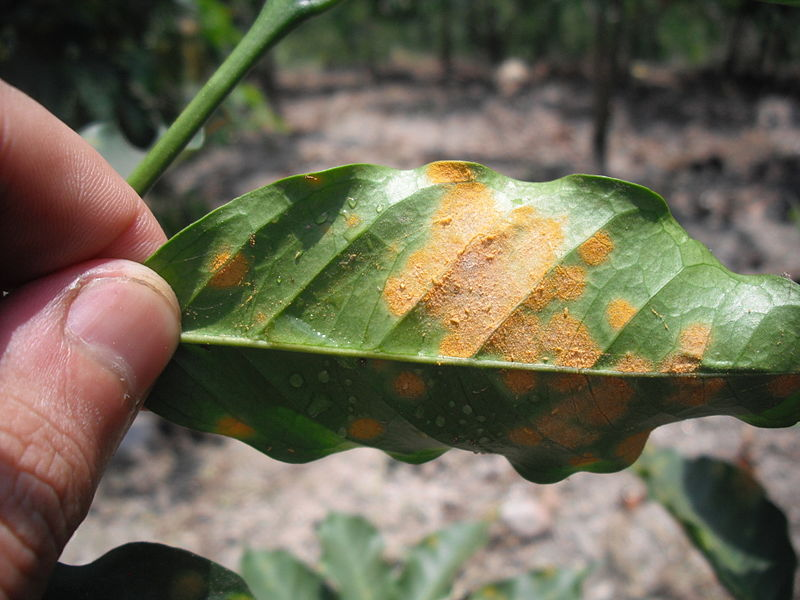
\includegraphics[width=0.8\linewidth]{./images/hemileia_vastatrix_coffee_leaf_rust} \end{center}

\textbf{Downy mildew of grapes}

Class: Oomycota
Order: Peronosporales

\emph{Plasmopara viticola}, also known as grape downy mildew, is considered to be the most devastating disease of grapevines in climates with relatively warm and humid summers. It was first observed in 1834 by Schweinitz on Vitis aestivalis in the southeastern United States. France was among the first of the European countries to gain experience in dealing with the pathogen. Within just a few years of the pathogen's introduction the French attempted to graft American root stock to their own vines in order to produce a more resistant strain of grape. Depending on the year, production of grapes in France has been estimated to have been reduced by as much as 50\%.

\begin{center}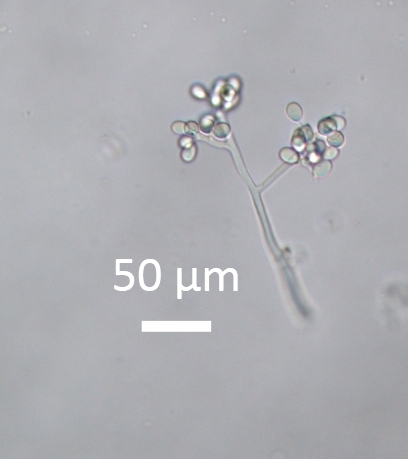
\includegraphics[width=0.8\linewidth]{./images/Plasmopara_vitticola} \end{center}

\textbf{Bengal famine of 1943}

The Bengal famine stroke Bengal province of British India during World war II. An estimated 2.1-3 million, out of a population of 60.3 million, died of starvation, malaria, or other diseases aggravated by malnutrition, population displacement and other causes. Affecting of winter rice with a severe outbreak of fungal brown spot disease ( \emph{Helminthosporium oryzae}) is considered to have a major role in the exacerbation of famine besides, political and other causes, cyclone particularly.

\hypertarget{rust}{%
\section{Rust}\label{rust}}

\hypertarget{management}{%
\subsection{Management}\label{management}}

Macrocyclic disease: \emph{Puccinia graminis} is a macrocyclic heteroecious fungus that causes wheat stem rust disease. The repeating stage in this fungus occurs on wheat and not the alternate host, barberry. The repeating stage allows the disease to persist in wheat even though the alternate host may be removed. Planting resistant crops is the ideal form of disease prevention, however, mutations can give rise to new strains of fungi that can overcome plant resistance. Although the disease cannot be stopped by removal of the alternate host, the life cycle is disrupted and the rate of mutation is decreased because of reduced genetic recombination. This allows resistance bred crops to remain effective for a longer period of time.

Demicyclic Disease: Because there is no repeating stage in the life cycle of demicyclic fungi, removal of the primary or the alternate host will disrupt the disease cycle. This method, however, is not highly effective in managing all demicyclic diseases. Cedar-apple rust disease, for example, can persist despite removal of one of the hosts since spores can be disseminated from long distances. The severity of Cedar-apple rust disease can be managed by removal of basidiospore producing galls from junipers or the application of protective fungicides to junipers.

Sulphur powder is known to stop spore germination. Fungicides such as Mancozeb and Triforine may help but may never eradicate the disease.

\hypertarget{common-rust-fungi-in-agriculture}{%
\subsection{Common rust fungi in agriculture}\label{common-rust-fungi-in-agriculture}}

\begin{itemize}
\tightlist
\item
  \emph{Hemileia vastatrix} (Coffee rust); Primary host is coffee plant; unknown alternate host. Heteroecious
\item
  \emph{Phakopsora meibomiae} and \emph{P. pachyrhizi} (Soybean rust); Primary host is soybean and various legumes. Unknown alternate host. Heteroecious
\item
  \emph{Puccinia coronata} (Crown Rust of Oats and Ryegrass); Oats are the primary host; Rhamnus spp. (Buckthorn) is alternate host. Heteroecious and macrocyclic
\item
  \emph{Puccinia graminis} (Stem rust of wheat and Kentucky bluegrass, or black rust of cereals); Primary hosts include: Kentucky bluegrass, barley, and wheat; Common barberry is the alternate host. Heteroecious and macrocyclic
\item
  \emph{Puccinia hemerocallidis} (Daylily rust); Daylily is primary host; Patrina sp is alternate host. Heteroecious and macrocyclic
\item
  \emph{Puccinia triticina} (Brown Wheat Rust) in grains
\item
  \emph{Puccinia sorghi} (Common Rust of Corn)
\item
  \emph{Puccinia striiformis} (Yellow Rust) of cereals
\item
  \emph{Uromyces appendiculatus} (Bean Rust) in common bean (Phaseolus vulgaris){[}16{]}
\item
  \emph{Puccinia melanocephala} (Brown Rust of Sugarcane)
\item
  \emph{Puccinia kuehnii} (Orange rust of Sugarcane)
\end{itemize}

\textbf{UG99}

It is a lineage of wheat stem rust ( \emph{Puccinia graminis f.~sp. tritici}), which is present in wheat fields in several countries in Africa and Middle east and is predicted to spread rapidly through these regions and possibly further afield, potentially causing a wheat production disaster that would affect food security worldwide. It can cause up to 100\% crop losses and is virulent against many resistance genes which have previously protected against stem rust.

\hypertarget{citrus-decline-in-nepal}{%
\subsection{Citrus decline in Nepal}\label{citrus-decline-in-nepal}}

Citrus greening disease or HLB was first reported from China in 1919 by Reinking while evaluating diseases of economic plants in southern China and used English term ``yellow shoot'' of citrus in the report. At that time it was believed that the HLB was caused by abiotic factors like Zn deficiency/toxicity and poor drainage system. By 1967, it became established that greening was graft and insect transmissible with conclusion caused by virus (Bove 2006). In 1967, mycoplasm like organisms (MLOs) were believed to be associated with plant diseases mostly with ``yellow'' symptoms resembling with greening symptoms. On close examination, these organisms were seen to have bacterial cell wall in addition to cytoplasmic membrane, suggesting that they were gram negative true bacteria (Garnier and Bove 1977). Thus, it was concluded that the HLB agent was gram negative bacterium -- \emph{Liberobacter asiaticus}.

Citrus decline was reported for the first time in Pokhara valley by Thrower (1968) in Nepal. Based on visual observation, Knorr et al (1970) suspected that the decline was caused by greening disease entered with the planting materials introduced to Horticulture Research Station, Pokhara from Saharanpur, India. About 55\% of citrus trees in Pokhara valley and 100\% in Horticulture Research Station were symptomatic to HLB in 1980s (Regmi 1982).

More recent PCR test showed that HLB is widespread in many citrus pockets of Kaski, Syanja, Tanahu, Lamjung and Dhading districts (Bove 2006 Regmi and Yadav 2007 Regmi et al 2010).

\textbf{Diagnosis of Citrus decline}

Visual symptoms are apparent on leaves and fruits. A tree infected with HLB in the field usually develops one or more yellow shoots with other parts of the tree healthy or symptomless. The affected leaves develop a pattern of yellow and green areas lacking clear limits between the colors, giving a ``blotchy mottle'' appearance. This is the most characteristic foliar symptom and the patterns are asymmetrical on the two halves of the leaf (Bove 2006). Leaves can also become thicker, with veins enlarged and corky in appearance. In later stages, Zn deficiency-like symptoms can be seen followed by leaf drop and twig dieback.

Currently, other methods besides visual diagnosis of Huanglongbang are molecular marker based test (quantative PCR), biological indexing, iodine test and spectroscopy. Based on severity of HLB symptoms and the ability to continue growth of the plants inoculation with \emph{Ca.} L. \emph{asiaticus} Folimonova et al (2009) grouped citrus genotypes into four categories as
i. sensitive: C. halimii, Nules clementine mandarin, Minneola tangelo, sweet oranges and grapefruit
ii. moderately tolerant: Sun Chu Sha mandarin, sour orange, volkamer lemon, C. macrophylla, wingle citrumelo, citron, Palestine sweet lime, acid lime, calamondin, and C. micrantha
iii. tolerant: Eureka lemon, Persian lime, Carrizo citrange, and Severinia buxifolia
iv. variable (some branch sensitive and some branch tolerant): pummelos, C. amblycarpa, cleopatra mandarin, C. indica, and meiwa kumquat.

\textbf{Citrus greening control}

\begin{itemize}
\item
  Inoculum reduction and vector control: Planting of certified clean planting materials, effective control of its vector psyllid populations and removal of infected trees that serve as an inoculums source for psyllid acquisition are the methods of choice. Biological control of the psyllid vector is only possible in locations that do not favour build-up of psyllid populations and is often compromised when hyper-parasites are present.
\item
  Chemical control: Combination of penicillin and streptomycin (PS) was effective in eliminating or supressing the bacterium.
\item
  Nutrition: Preliminary results of the research showed that HLB-infected trees are consistently deficient in Ca, Mg, Mn, Zn and B, and in an orchard. The main cause of visible HLB symptoms, yield reduction, and tree decline appears to be disruption of phloem tissue, which blocks the flow of photosynthate and nutrients from source to sink tissue. Hence plant growth enhancers, mainly that of root system should, to some extent, alleviate the symptoms of HLB.
\item
  Use of tolerant rootstocks: The citrus rootstock US-897 ( \emph{Citrus reticulata} Blanco x \emph{Poncirus trifoliata} L. Raf.) was observed to be tolerant to HLB in field plantings.
\item
  Guava intercropping: An observation in Vietnam in 2000, noted that the normal life of sole citrus plantings in Mekon region was 2 to 4 years, but those interplanted with white guava were surviving for up to 15 years (Gottwald et al 2010). Raising guava as an intercrop reduced psyllid population in citrus orchards.
\end{itemize}

\hypertarget{guava-wilt}{%
\subsection{Guava wilt}\label{guava-wilt}}

Causative agent: \emph{Fusarium oxysporium f.~psidi}, \emph{Rhizoctonia spp.}

Guava plants are attacked by wilt causing pathogen, which alone causes heavy losses in Nepalese guava trees. Yellowing and browning of leaves from the twigs tip. Leaves die off causing cracking in the twigs and trunk leading to the complete wilting and decline of entire tree. The incidence is more severe in alkaline soil and during winter season.

\textbf{Control measures}

\begin{itemize}
\tightlist
\item
  It is better to remove such trees as soon as the symptoms are identified to prevent the spread of disease.
\item
  Apply 15 gm of bavistin at the basin of each plant after pruning in March, June and September.
\item
  Liming of the pits.
\item
  Use of resistant root stock such as chinese guava and wilt resistant variety like Allahabad safeda, Banarasi, Nasik etc.
\end{itemize}

\hypertarget{fruit-rot-of-guava}{%
\subsection{Fruit rot of guava}\label{fruit-rot-of-guava}}

Causative agent: \emph{Phomopsis psidi}

This is a serious disease especially during rainy seasons. The symptoms are manifested as development of dark brown circular spots at the blossom end of the immature green fruits.

Control measures: Application of Zineb (0.2\%) or aureofungin (10 ppm) as monthly sprays during June to October can control the disease. Apply Kavach/Rovral (2g/ltr) and Carbendazim (1 g/ltr) during rainy season.

\hypertarget{fruit-canker}{%
\subsection{Fruit canker}\label{fruit-canker}}

Causative agent: \emph{Pestalotiopsis psidi}

Cankerous growth on fruit leading to cracking of fruits.

Control measures: Apply Dilhan 278 (2g), Cuman L (4 ml/ltr) and Rovral (2g/ltr) during rainy season.

\hypertarget{chirke-and-furket-of-cardamom}{%
\subsection{Chirke and furket of Cardamom}\label{chirke-and-furket-of-cardamom}}

\hypertarget{downy-mildew-of-cucumber}{%
\subsection{Downy mildew of cucumber}\label{downy-mildew-of-cucumber}}

\hypertarget{stemphyllium-blight-of-lentil}{%
\subsection{Stemphyllium blight of lentil}\label{stemphyllium-blight-of-lentil}}

\hypertarget{root-knot-nematode-of-tomato-brinjal-and-ladys-finger}{%
\subsection{Root knot nematode of Tomato, Brinjal and Lady's finger}\label{root-knot-nematode-of-tomato-brinjal-and-ladys-finger}}

\hypertarget{section}{%
\section{}\label{section}}

\begin{itemize}
\tightlist
\item
  A popular fungicide, generally used for seed treatment, called Carbendazim is available in commercial formualtion as KI-BESTIN (Carbendazim 50\% WP).

  \begin{itemize}
  \tightlist
  \item
    The commercial seed treatment fungicide is composed of:

    \begin{itemize}
    \tightlist
    \item
      51\% Carbendazim 98\% (at minimum) a.i.
    \item
      2\% Surface acting agent
    \item
      2\% Dispersing agent
    \item
      2\% Sticking agent (Glue powder)
    \item
      43\% Inert carrier (China clay)
    \end{itemize}
  \item
    In case of carbendazim poisoning medical charcoal preparation 6-10 times is recommended.
  \item
    It has green colored warning level.
  \item
    It is manufactured by Kisan Agro Chemicals, Parsa, Birgunj, Nepal.
  \item
    KI-BESTIN is a broad spectrum systemic fungicide useful as both spray and wetted powder form.
  \end{itemize}
\end{itemize}

\hypertarget{biopesticides}{%
\section{Biopesticides}\label{biopesticides}}

\begin{itemize}
\tightlist
\item
  \emph{Nisarga}

  \begin{itemize}
  \tightlist
  \item
    Active ingredient: \emph{Trichoderma viridae}
  \item
    Effectiveness: Stem rot, Root rot, Sett rot, Damping off, Ganoderma etc. Against \emph{Fusarium}, \emph{Sclerotium}, \emph{Phytopthora} and \emph{Ganoderma}.
  \item
    Utility crops: Potato, tomato, sweet pepper, garlic, cauliflower, onion, tea, coffee and pulses.
  \item
    Dosage: Spray 5 gm Nisarga per liter of water solution. While applying in soil, 500 gm Nisarga is mixed with 2.5 kg of mature FYM or compost. This suffices for 1 ropani of land.
  \end{itemize}
\item
  \emph{Pseudomonas}

  \begin{itemize}
  \tightlist
  \item
    Active ingredient: \emph{Pseudomonas fluorescence}
  \item
    Effectiveness: Onion smut, Paddy blast, Bacterial wilt of pepper and Dieback of tomato.
  \item
    Useful against soil borne, seed borne and air borne pathogens.
  \item
    Secondary metabolites, i.e.~Auxin, Gibberelic acid and Cytokinins promote plant health.
  \item
    Dosage: Spray 5 g of Pseudomonas commercial formula in 1 liter of water. While applying in soil, 500 gm Nisarga is mixed with 2.5 kg of mature FYM or compost. This suffices for 1 ropani of land.
  \end{itemize}
\item
  Verticillium fungicide is effective against sucking insects and nematodes.

  \begin{itemize}
  \tightlist
  \item
    In a ropani of land, use 500 gm of verticillium preparation with 2.5 kg of FYM/compost.
  \end{itemize}
\item
  Neem Baan

  \begin{itemize}
  \tightlist
  \item
    Contains Azadirachtin.
  \item
    Effectiveness: Against phytophagous insects for deterrence. It inhibits oviposition and is ovicidal (kills larvae if hatched)
  \item
    Most effective against sap sucking type insects (Aphid, mealy bug, white fly, thrips, etc.) and chewing type insects (Stem and fruit borer larvae)
  \item
    Has contact and systemic property
  \item
    Dosage: 2-5 ml liquid in 1 ltr of water is sprayed in 12 days interval, 2-3 times.
  \item
    Composition: 0.03\%, 0.15\%, 1\%, etc.
  \end{itemize}
\item
  Nuclear polyhedrosis virus (NPV)
\item
  Granulosis virus (GVs)
\end{itemize}

\hypertarget{pathogens}{%
\section{Pathogens}\label{pathogens}}

\hypertarget{nematodes}{%
\subsection{Nematodes}\label{nematodes}}

\begin{itemize}
\item
  Nematode is derived from the Greek words, ``Nema'' = thread/fibre, ``toda'' = worm.
\item
  In germany, there is a separate University of Nematology.
\item
  Nematodes can be defined as unsegmented, bilaterally symmetrical, tryploblastic, pseudocoelomate, invertebrate, and thread like worms.
\item
  So far 50000 nematode species are recorded worldwide. 10000 are found in fresh water and soil. 300 species are known to be plant parasites.
\item
  Molya disease ( \emph{Heterodera avenae}) causes 6-7 crore/year loss in Rajasthan and ear cockle ( \emph{Anguina tritici}) causes 8 crore loss in India.
\item
  \emph{Radopholus similis} was found associated with citrus decline in Florida, USA.
\item
  In India, \emph{Tylenchulus semipenetrans} was associated with citrus decline.
\item
  Plant parasitic nematodes are triploblastic, bilaterally symmetrical, unsegmented, pseudocelomate and vermiform animals.
\item
  The body of the nematode may be elongated, spindle shaped, fusiform tapering towards the end but the cross section is always circular.
\item
  Smallest nematode is 10mm long ( \emph{Paralongidorus}).
\item
  Female nematodes are more virulent and agressive than male in attacking and parasitizing the plants.
\item
  Plant parasitic nematode possess spear or stylet.
\item
  Nematodes are known to transmit viruses:

  \begin{itemize}
  \tightlist
  \item
    Two single stranded RNA virus genera, Nepovirus (NEPO) and Tobravirus (TOBRA).
  \item
    11 species of Xiphinema transmit 13 NEPO virus (Grapevine fan leaf virus)
  \item
    11 species of Longidorus transmit 10 NEPO virus
  \item
    14 species of Trichodorus transmit various strains of TOBRA virus: tobacco rattle and pea early browning
  \end{itemize}
\end{itemize}

Insect transmitted viruses

\begin{table}

\caption{\label{tab:insect-transmissed-viruses}Insect mediated virus transmission}
\centering
\begin{tabular}[t]{ll}
\toprule
Virus & Nematode\\
\midrule
Rice dwarf virus & Nephotettix cincticeps\\
Rice tungro virus & Nephotettix impicticeps\\
Rice grassy stunt virus & Nilaparvata lugens\\
Tomato spotted wilt virus & Thrips tabaci, Frankliniella spp.\\
Tomato yellow leaf curl virus & Bemisia tabaci\\
\addlinespace
Tomato yellow mosaic virus & Bemisia tabaci\\
Soybean yellow mosaic & Bemisia tabaci\\
Grapevine virus A & Pseudococcus longispinus (Mealybugs)\\
Cowpea mosaic virus & Epilachna varivestis\\
Potato virus X virus & Melanoplus differentialis (Grasshopper)\\
\addlinespace
Tobacco mosaic virus & Liriomyza langei (Leafminer); Mechanical transmission\\
Onion mosaic virus & Eriophyses tulipae (Mites)\\
Soybean mosaic virus & Aphids\\
Potato leaf roll virus & Myzus persicae\\
\bottomrule
\end{tabular}
\end{table}

\hypertarget{crop-diseases}{%
\section{Crop diseases}\label{crop-diseases}}

\hypertarget{ergot-wheat-barley-oats-rye-triticale}{%
\subsection{Ergot (Wheat, barley, oats, rye, triticale)}\label{ergot-wheat-barley-oats-rye-triticale}}

Hosts:
All grasses, particularly, blackgrass ( \emph{Alopecurus myosuroides})

Symptoms:
- Causal fungus only attacks ears of flowering, replacing the grain in a few spikelets by a hard, purple black sclerotium, known as ergot.
- Such ergots can be very large, upto 2 cm in length, and very obvious in the standing crop in contaminated grain samples.

Life cycle:
- Ergot is not truely a seed borne disease, however it can be spread by ergots in contaminated seeds.
- At or near harvest, ergots fall to the ground where they remain untill the following summer, when they germinate to produce club-shaped spore bearing structure (stroma). These ascospores are spread by the wind to nearly open flowers of grasses/cereals. The spores germinate in flower, infecting the ovaries. This infection leads to the production of secondary spores (condia) encased in sticky secretion commonly referred to as honeydew. This attracts insects which carry the spores to other flowers, where further infection can occur.
- Wheat and other cereals are less severely affected than rye although, occassionally more open-flowerd wheat variety can be badly affected.
- Disease is favored by cool, wet conditions during flowering which facilitate spore production and prolong the flowering period, making infection more likely.

Importance:
- Very little direct effect on yield.
- Affects stocks which when fed to flour made with cereals with large amount of toxic alkaloid containing ergot, possess health risks.

\hypertarget{fusarium}{%
\subsection{Fusarium}\label{fusarium}}

Fusariusm head blight/ear blight, foot rot, seedling blight
Pathogen: \emph{Fusarium spp.} and \emph{Microdochium nivale}
Hosts: Wheat, barley, oats, rye triticale and grasses.

Symptoms:
- Form a complex of diseases on seeds, seedlings and adult plants.
- \emph{Microdochium nivale} (formerly known as \emph{Fusarium nivale}) is seed-borne pathogen and causes seedling blight resulting in seedling death and thinning of plant stand.
- \emph{M. spp} (other than \emph{M. nivale}) cause a range of symptoms including brown lesions on stem bases, often restricted to outer leaf sheath.
- \emph{Fusarium lesions} often begin in the leaf sheath at the stem base where crown roots split the leaf sheath when emerging.
- This infection can spread up the leaf sheath causing long dark brown streaks at the stem base. The other symptom in cooler regions is brown staining of lower nodes.
- In older plants, fusarium infection can produce a true foot rot, where the stem base becomes brown and rotten, resulting in lodging and white heads.
- Symptoms are prevalent in very dry seasons as well.
- Ear blight causing fungus: \emph{F culmorum} and \emph{F graminearum} are common. Other are, \emph{F avenaceum}, \emph{F poae} and \emph{F langsethiae}.
- Infection frequently results in the whole or part of the ear becoming bleached.
- Symptoms seen when ears become infected during the early flowering stages, later infection may result in infection of grain but without obvious bleaching of the ears.
- Important due to its mycotoxin that gets accumulated in grains.

Life cycle:
- Most important source is seed but fungus survives on debris in soil also.
- Spores are splashed in canopy causing ear blights and seed borne infection, in wet seasons, especially during flowering and grain formation.
- Most fusarium species have competative saprophytic abilities which allow them to colonize debris and stubble in soil.

Importance:
- When wet season coincides with flowering high levels of ear blight can occur.
- Due to seed borne nature of pathogen, seed treatment plays role in preventing seedling loss in wheat.

\hypertarget{major-diseases-of-rice}{%
\subsection{Major diseases of rice}\label{major-diseases-of-rice}}

\begin{enumerate}
\def\labelenumi{\arabic{enumi}.}
\tightlist
\item
  Blast
\end{enumerate}

\begin{itemize}
\tightlist
\item
  Bavistin, Dorosal 2-3 g per kg seed treatment
\item
  Tricyclazole 75\% WP 0.75 g per ltr spray at 15 days interval
\item
  Kasugamycin 3\% SL 1.5 ml per ltr at 15 days interval
\end{itemize}

\begin{enumerate}
\def\labelenumi{\arabic{enumi}.}
\setcounter{enumi}{1}
\tightlist
\item
  Bacterial leaf blight
\end{enumerate}

\begin{itemize}
\tightlist
\item
  Use Agromycin-100 0.25 g per ltr for seed soaking for 30 minutes
\end{itemize}

\begin{enumerate}
\def\labelenumi{\arabic{enumi}.}
\setcounter{enumi}{2}
\tightlist
\item
  Brown leaf spot disease
\end{enumerate}

\begin{itemize}
\tightlist
\item
  Bavistin, Dorosal
\item
  Apply Mancozeb 75\% WP (Dithane M-45) 3 g per ltr water, Propineb 70\% WP 3 g per ltr water at 15 days interval for 3 times.
\end{itemize}

\begin{enumerate}
\def\labelenumi{\arabic{enumi}.}
\setcounter{enumi}{3}
\tightlist
\item
  Foot rot
\end{enumerate}

\begin{itemize}
\tightlist
\item
  Carbendazim 50\% WP seed treatment
\end{itemize}

\begin{enumerate}
\def\labelenumi{\arabic{enumi}.}
\setcounter{enumi}{4}
\tightlist
\item
  Sheath blight
\end{enumerate}

\begin{itemize}
\tightlist
\item
  Maintain spacing
\item
  Validamycin 3\% L 3 g per ltr water; Pencycuron 22.9 SC 1.5 ml per ltr; Carbendazim 70\% WP 1.5 g per ltr spray at 10-12 days interval for two times.
\end{itemize}

\begin{enumerate}
\def\labelenumi{\arabic{enumi}.}
\setcounter{enumi}{5}
\tightlist
\item
  Khaira disease
\end{enumerate}

\begin{itemize}
\tightlist
\item
  20 g \(\mathrm{ZnSO_4}\) + 12\% \(\mathrm{CaCO_3}\) in 50 ltr water per ropani at 10 days interval for 2 times.
\end{itemize}

\hypertarget{major-diseases-of-wheat}{%
\subsection{Major diseases of Wheat}\label{major-diseases-of-wheat}}

\begin{enumerate}
\def\labelenumi{\arabic{enumi}.}
\tightlist
\item
  Leaf blight
\end{enumerate}

\begin{itemize}
\tightlist
\item
  Small brown dots on leaves
\item
  Later on the dots coalesce to cause wilting or blighted appearance
\item
  Use Vitavex-200 2 gm per kg seed as presowing treatment
\item
  Increase potassium fertilizer dosage
\end{itemize}

\begin{enumerate}
\def\labelenumi{\arabic{enumi}.}
\setcounter{enumi}{1}
\tightlist
\item
  Brown rust
\end{enumerate}

\begin{itemize}
\tightlist
\item
  Orange color spots on upper surface of leaves.
\item
  Spots do not coalesce or merge
\item
  Mancozeb (Dithane M-45 45 WP) 1.5-2 kg in 750 ltr water spray at interval of 15 days for 2-3 times.
\end{itemize}

\begin{enumerate}
\def\labelenumi{\arabic{enumi}.}
\setcounter{enumi}{2}
\tightlist
\item
  Yellow rust
\end{enumerate}

\begin{itemize}
\tightlist
\item
  Yelow colored spots, elongated and jointed to form stripes
\item
  Cultivation of resistant varieties: WK-1204, Pasang Lhamu.
\end{itemize}

\begin{enumerate}
\def\labelenumi{\arabic{enumi}.}
\setcounter{enumi}{3}
\tightlist
\item
  Loose smut
\end{enumerate}

\begin{itemize}
\tightlist
\item
  Instead of grains black mass of fungal hyphae fills the panicle.
\item
  Use of healhty seeds, Vitavex-200 2 g per kg seed treatment
\item
  Bury the sick panicles in initial stage of disease appearance.
\item
  Annapurna variety is relatively tolerant to disease.
\end{itemize}

\begin{enumerate}
\def\labelenumi{\arabic{enumi}.}
\setcounter{enumi}{4}
\tightlist
\item
  Stinking smut/hill smut
\end{enumerate}

\begin{itemize}
\tightlist
\item
  Diseased grains are rounded, black colored spores filled
\item
  Spores only released after grain is crushed
\item
  Smell of fish
\item
  Crop rotaion for 2-3 years, Vitavex-200 2 g per kg seed treatment.
\end{itemize}

\hypertarget{major-diseases-of-jackfruit}{%
\section{Major diseases of jackfruit}\label{major-diseases-of-jackfruit}}

\begin{enumerate}
\def\labelenumi{\arabic{enumi}.}
\tightlist
\item
  Pink disease ( \emph{Botryobasidium salmonicolor})
\end{enumerate}

\hypertarget{entomology}{%
\chapter{Entomology}\label{entomology}}

\hypertarget{pesticide-toxicity}{%
\section{Pesticide toxicity}\label{pesticide-toxicity}}

\begin{itemize}
\item
  A pesticide is any substance used to control pests. Pests may be target insects, vegetation, fungi, etc. Most control the pests by poisoning them. Unfortunately, pesticides can be poisonous to humans as well.
\item
  Toxicity: The toxicity of a substance is its capacity to cause injury to a living system. A living system can be things such as a human body, parts of the body (lungs or respiratory system), a pond, a forest and those creatures that live in there. Toxicity represents the kind and extent of damange that can be done by chemical. In other words, if you know the toxicity of a pesticide, you know how poisonous it is.
\item
  Dose-time relationship of pesticide toxicity

  \begin{itemize}
  \tightlist
  \item
    Dose is the quantity of a substance that a surface, plant or animal is exposed to.
  \item
    Time means how often the exposure occurs.
  \item
    This relationship gives rise to two types of toxicity.
  \end{itemize}

  \begin{enumerate}
  \def\labelenumi{\arabic{enumi}.}
  \tightlist
  \item
    Acute toxicity: This refers to how poisonous a pesticide is to a human, animal or plant after a single-term exposure. It generally implies the effect that occurs within 24 hours of exposure.
  \item
    Chronic toxicity: This refers to delayed poisonous effects from exposure to substance.
  \end{enumerate}
\item
  Routes of entry:

  \begin{enumerate}
  \def\labelenumi{\arabic{enumi}.}
  \tightlist
  \item
    Local: local effect refers to those that take place at the site of contact with material. e.g.~skin irritation/inflammation on th hand in response to hand contact, irritation of mucous membrane lining the lungs due to inhalation of toxic fumes.
  \item
    Systemic: Effect that occur away from the original point of contact. These pesticides are distributed throughout the body once they enter. They function by blocking or stimulating a chemical signal, generally that of the nervous system (Cholinesterase).
  \end{enumerate}
\item
  Pesticides may have following actions:
\item
  Additive, antagonistic or synergistic
\item
  Immediate or delayed
\item
  Reversible or irreversible action
\item
  Exposure may result in following effects:

  \begin{itemize}
  \tightlist
  \item
    Reproductive effects
  \item
    Teratogenic effects: Effect on unborn offspring, such a birth defects.
  \item
    Carcinogenic effects: Cancer in living animal tissues.
  \item
    Oncogenic effects: Tumor forming effect (not necessarliy cancerous)
  \item
    Mutagenic effects: Permanent effect on genetic material that can be inherited
  \item
    Neurotoxicity: Poisoning of nervous system, including the brains.
  \item
    Immunosupression
  \end{itemize}
\end{itemize}

Acute toxicity measures

To figure out how acutely toxic a pesticide is, scientists give laboratory animals short-exposure to does of pesticide being tested. Experimental doses are given orally, as well as put on eyes, skin, and in the air that test animals breathe. These animals are then carefully observed for the changes.

\textbf{LD50}

Amount of a pesticide that has killed half of the animals in a laboratory test. LD50 values are effective for both oral and dermal routes of exposure. But they do not tell us about how the chemical acts, nor about how sensitive different organs within an animal or human might be. LD50 for different chemicals can be compared if the same test animial was used. The LD50 values are measured in unit of weight called mg per kg (or interchangeably, parts per million).

\textbf{LC50}

This measure of toxicity gives the acute inhalation toxicity.

Chronic toxicity measures

There is no standard measure like LD50 for chronic toxicity studies. Often the length of the experiment is in days, months or years and the amount of each dose is stated. For e.g., a study of chronic oral toxicity might look like, ``8 mg of pesticide to rats daily for two years. No symptoms of poisoning appeared.''

\begin{itemize}
\tightlist
\item
  Two classes of pesticides, organophosphates and carbamates can slowly poison by attacking an essential body chemical called ``cholinesterase''. The chronic exposure to Organophosphate pesticides can be measured by monitoring changes in blood cholinesterase levels. In humans, decrease in cholinesterase levels are sure sign that exposure to these types of pesticides should be avoided untill the level is measured as being normal again.
\end{itemize}

Categories of pesticide toxicity

\begin{table}

\caption{\label{tab:pesticide-hazard-category}Categories of pesticide toxicity}
\centering
\begin{tabular}[t]{lllll}
\toprule
Toxicity class & Toxicity label & Oral LD50 (mg/kg) & Dermal LD50 (mg/kg) & Inhalation LC50 (mg/L)\\
\midrule
Highly toxic & Danger & 0-50 & 0-200 & 0-0.2\\
Moderately toxic & Warning! & 50-500 & 200-2000 & 0.2-2\\
Slightly toxic & Caution!! & 500-5000 & 2000-20000 & 2-20\\
Relatively non-toxic & Caution!! & >5000 & >20000 & >20\\
\bottomrule
\end{tabular}
\end{table}

Status of pesticide use in Nepal

\begin{itemize}
\tightlist
\item
  Initially, DDT was imported in 1952 AD for control of Maleria.
\item
  For the same purpose, DDT was reimported in 1955 AD
\item
  For use in crops, DDT was imported in 1956 AD.
\item
  According to Thapa, 2003, average pesticide use in Nepal is 142 gm/ha.
\item
  In general, cropwise analysis of pesticide use signals alarming levels of residues, hence their current state of use being haphazard.

  \begin{itemize}
  \tightlist
  \item
    Tea: 2100 gm/ha
  \item
    Cotton: 2560 gm/ha
  \item
    Vegetables: 1400 gm/ha
  \end{itemize}
\item
  On environmental perspective, pesticides are of following types, based on bio-degradation:

  \begin{enumerate}
  \def\labelenumi{\arabic{enumi}.}
  \tightlist
  \item
    Environmentally degradable/non-persistent:
  \end{enumerate}

  \begin{itemize}
  \tightlist
  \item
    Dimethoate (Nuger, Roger, Dimet)
  \item
    Dichlorovos (Dum, Vapon)
  \item
    Fenitrothion (Folithion)
  \item
    Malathion
  \end{itemize}

  \begin{enumerate}
  \def\labelenumi{\arabic{enumi}.}
  \setcounter{enumi}{1}
  \tightlist
  \item
    Environmentally non-degradable/persistent:
  \end{enumerate}

  \begin{itemize}
  \tightlist
  \item
    PoPs: Aldrin, chlordane, DDT, Dialdrin, Eldrin, Heptachlor, Mirex, Toxaphene, HCB, PCB, Dioxyn, Furan, etc.
  \item
    These pesticides require special treatment facility for disposal.
  \end{itemize}
\end{itemize}

\hypertarget{major-insects-of-rice}{%
\section{Major insects of rice}\label{major-insects-of-rice}}

\begin{enumerate}
\def\labelenumi{\arabic{enumi}.}
\tightlist
\item
  Seed bed bettle, mole cricket, field cricket
\item
  Borer
\item
  Rice hispa
\item
  Hoppers
\item
  Rice bug
\item
  Leaf roller
\item
  Mealy bug
\end{enumerate}

\hypertarget{major-insects-of-wheat}{%
\section{Major insects of wheat}\label{major-insects-of-wheat}}

\begin{enumerate}
\def\labelenumi{\arabic{enumi}.}
\tightlist
\item
  Larvae of wireworm
\end{enumerate}

\begin{itemize}
\tightlist
\item
  Similar to cutworm in Maize (damages the crop at night)
\item
  Use Bt for control
\item
  Malathion 5\% DP 2 g per kg with wheat bran 1/2 kg per ropani, during evening
\item
  Chlorpyrifos 10\% Granule or Malathion 5\% DP 1 kg per ropani for soil treatment
\end{itemize}

\begin{enumerate}
\def\labelenumi{\arabic{enumi}.}
\setcounter{enumi}{1}
\tightlist
\item
  Aphid
\end{enumerate}

\begin{itemize}
\tightlist
\item
  Lady bird beetle is its natural enemy
\item
  Dimethoate 30\% EC 1 ml per liter water
\end{itemize}

\begin{enumerate}
\def\labelenumi{\arabic{enumi}.}
\setcounter{enumi}{2}
\tightlist
\item
  Pink stem borer
\end{enumerate}

\begin{itemize}
\tightlist
\item
  Same as that for control of Maize stem borer
\end{itemize}

\hypertarget{major-insects-of-tomato}{%
\section{Major insects of tomato}\label{major-insects-of-tomato}}

\hypertarget{leaf-miner-of-tomato-tuta-absoluta}{%
\subsection{\texorpdfstring{Leaf miner of tomato ( \emph{Tuta absoluta})}{Leaf miner of tomato ( Tuta absoluta)}}\label{leaf-miner-of-tomato-tuta-absoluta}}

The tomato leafminer (aka. Tomato pinworm and South American tomato moth) is a species of moth in family Gelechiidae. \emph{T. absoluta} was originally described in 1917 by Meyrick as \emph{Phthorimaea absoluta}. The pest was finally described under the genus Tuta as \emph{T. absoluta} by Povolny in 1994. In India, Maharashtra state tomato cultivation were affected in Nov 2016.

Its life-cycle comprises four development stages: egg, larva, pupa and adult. Adults usually lay eggs on the underside of leaves or stems, and to a lesser extent on fruits. Adult female live 10-15 days and male live 6-7 days.

After hatching, young larvae penetrate leaves, aerial fruits (like tomato) or stems, on which they feed and develop. Larvae drop to the ground in a silken thread and pupate in soil. Pupae (length: 5--6 mm) are cylindrical in shape and greenish when just formed becoming darker in colour as they are near adult emergence. Adults are 6--7 mm in length and present filiform antennae and silver to grey scales. Black spots are present on anterior wings, and the females are wider and more voluminous than the males. The adult moth has a wingspan around 1 cm. In favorable weather conditions eight to ten generations can occur in a single year.

\begin{center}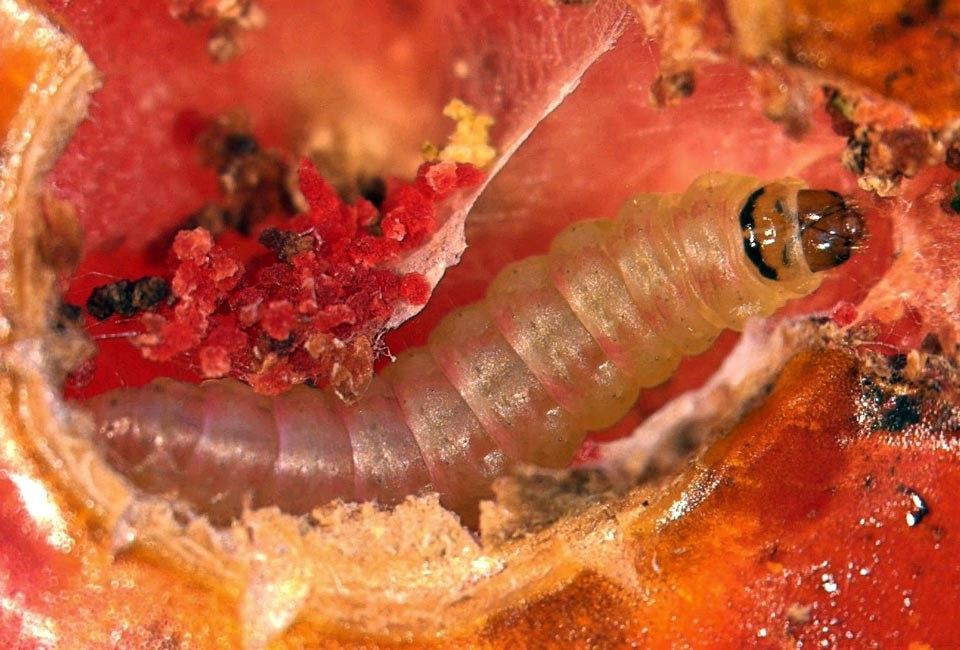
\includegraphics[width=0.8\linewidth]{./images/tuta_absoluta} \end{center}

The pest mainly presents nocturnal habits, and adults usually remain hidden during the day, showing greater morning-crepuscular activity with adults dispersing among crops by flying. Among a range of species within the Solanaceae, tomatoes ( \emph{Lycopersicon esculentum} Miller) appear to be the primary host of \emph{T. absoluta}.

\textbf{Management}

\begin{itemize}
\tightlist
\item
  Removing and destruction of infested plant parts. Tomato is the main host of the plant, but \emph{T. absoluta} also attacks other plants of the nightshade family -- Potato, eggplant, pepino, pepper and tobaccoo, including solanaceous weeds like \emph{Datura stramonium} and \emph{S. nigrum}.
\item
  Deep ploughing in spring season followed by solarization of field.
\item
  Continuous irrigation and inundating of field can help prevent pupation.
\item
  Crop rotation
\item
  Use of exclusion net (especially in nursery condition); Mesh size of less than 1.6 mm is recommended.
\item
  Use of sticky trap and light traps and yellow delta trap are useful in monitoring of \emph{T. absoluta} populations.
\item
  Para-pheromone TLM lure in Wota-T traps. The para-pheromone traps are used to monitor the adult moths. 5 Wota-T traps/ropani or 1 light trap/ropani.
\item
  Quarantine measures
\item
  Neem based pesticides (Neem raj), Jholmol botanicals
\item
  Imidacloprid, Emamectin benzoate (KINGSTAR, EMAR), Chlorantaniliprole (ALLCORA and CORAGEN) 18.5\% EC 1 ml per 3 ltr of water sprayed every 10-15 days, Spinosad (TRACER) 45\% SC 1 ml per 3 ltr water sprayed every 10-15 days, Chlorpyriphos and Cypermethrin.
\item
  Chlorantaniliprole, Spinosad and Flubendiamide (ryanoid class) all have waiting period of 7 days, while Emamectin benzoate, ranked as Moderately hazardous has waiting period of 10 days.
\item
  \emph{Bacillus thuringiensis kurstaki} (1\% WP 2 g per 1 ltr water sprayed every 7 days) have shown some efficiacy in controlling outbreaks of this moth. Similarly, \emph{Metarrhizium anisopliae} (\(1 \times 10^8\) CFU per gram ) 200-250 gm per ropani can be used for soil treatment.
\end{itemize}

\textbf{Monitoring of pest}

Crop damage should be monitored every two weeks. If noted abnormal minining in the leaf, with signs of mesophyll tissues being eaten and transparent veins exposed, suspect for presence of larvae of the pest. Tips of plant should show black massess, an indication of insect excreta. Fruits may show irregular strips of white coloration initially. In severe infestation, whole plant may appear as wilted. The larvae of Tuta will not enter diapause unless food is scarce. It is identifiable with characteristic pink colored body of 0.9 cm having half crescent rings like appearance in head.

\hypertarget{major-insects-of-guava}{%
\section{Major insects of guava}\label{major-insects-of-guava}}

\begin{itemize}
\tightlist
\item
  Fruit fly ( \emph{Dacus dorsalis})
\item
  Green shield scale ( \emph{Chloropulvinaria psidii})
\item
  Mealy bugs ( \emph{Ferrisia virgata}, \emph{Plannococcus citri})
\end{itemize}

\hypertarget{major-insects-of-jackfruit}{%
\section{Major insects of jackfruit}\label{major-insects-of-jackfruit}}

\begin{enumerate}
\def\labelenumi{\arabic{enumi}.}
\tightlist
\item
  Shoot and fruit borer ( \emph{Diaphania caesalis})
\item
  Giant mealy bug ( \emph{Drosicha mangiferae})
\end{enumerate}

\hypertarget{major-insects-of-litchi}{%
\section{Major insects of litchi}\label{major-insects-of-litchi}}

\begin{enumerate}
\def\labelenumi{\arabic{enumi}.}
\tightlist
\item
  Fruit borer ( \emph{Cryptophlebia illepida}, \emph{Rapala varuna}, \emph{Deudorix epijarbas}, \emph{Deudorix isocrates})
\item
  Fruit fly ( \emph{Bactrocera dorsalis})
\end{enumerate}

\hypertarget{biochemistry-and-biotechnology}{%
\chapter{Biochemistry and biotechnology}\label{biochemistry-and-biotechnology}}

\hypertarget{miscellaneous}{%
\chapter{Miscellaneous}\label{miscellaneous}}

\hypertarget{general}{%
\section{General}\label{general}}

\begin{itemize}
\item
  Kathmandu University was established in 2048 B.S.
\item
  Province 2 has the highest population density.
\item
  ``Time zero'' (Sunnya samaya) was written by Yubraj Ghimire.
\item
  According to 2068 survey, there are 64.63\% mobile phone users.
\item
  Padmashree literature accolade of 2075 was handed to Ramesh Sayaan's ``Chutteka Anuhar''
\item
  Padmashree sadhana accolade of 2075 was handed to historian Maheshraj Panta.
\item
  Minestrial cabinet first held their meeting with video conference in 2076, Bhadra 9.
\item
  The hurricane that struck Bara-Parsa in Bhadra 8 was named Dhumrapat.
\item
  Mr.~Surendra Prasad Yadav was appointed chairman of Civil Service Commission of Province 2 on Bhadra 5.
\item
  ``Yuva Moti Puraskar'' of 2075 was given to Shankar Chapagain (Dhankute Kancha) and Fulman Bal.
\item
  Nepal Government's legal advisor is Chief Justice (``Mahanyadibakta'')
\item
  Gautam Buddha communicated his learnings for 45 years.
\item
  Brazil is the country where sour honey can be found. ?
\item
  In San Marino, there are two presidents.
\item
  Moroccoo is the country where Red Salt is found.
\item
  In the Shree-Swasthani Puran (a branch of Skanda puran), there are 8110 slokas.
\item
  Full name of ``Ohm'' is George Simon Ohm.
\item
  Nepals goals (by):

  \begin{itemize}
  \tightlist
  \item
    Ending child marriage: 2020 AD
  \item
    Filariasis parasite eradication: 2020 AD
  \item
    Transition to developing country status: 2022 AD
  \item
    Birth rate substitution: 2022 AD
  \item
    Doubling tiger's population: 2022 AD
  \item
    Eradication of hunger: 2025 AD
  \item
    Malaria eradication: 2025 AD
  \item
    Hydroelectricity independence: 2027 AD
  \item
    Ending of poverty: 2030 AD
  \item
    Middle income status achievement: 2030 AD
  \end{itemize}
\item
  Which was the disease to be completely eradicated from the world: Measles.
\item
  During Rana regime, transaction of gold, silver and valuables was done by ``Bintipatra Niksari Adda''.
\item
  Ancientmost religion of Nepal is the ``Saiba''
\item
  Annual population growth rate was highest in 2038 BS.
\item
  Article 242 of Nepal's constitution has provision for civil serivce commission.
\item
  ``Urab'' is the caste that is recognized by its occupation of farming.
\item
  India launched the Chandrayan-2 rocket on July 22, 2019.
\item
  Madan puraskar, 2075 was awarded to Yogesh Raj's ``Ranahar''.
\item
  Jagadamba shree prize, 2075 was awarded to Bairagi kaila (Til Bikram Nembang).
\item
  Ministry of Civil Aviation and Tourism was chaired by Yogesh Bhattarai in Shrawan 15, 2076.
\item
  International Youth Year, 2019 had slogan: ``Transforming education''
\item
  Shuvadra Adhikari (Actress) died in Shrawan 32, 2076.
\item
  Indian foreign minister Shusma Shwaraj died on August 6, 2019.
\item
  Province number 5 was the earliest among provinces to appoint Civil Service Commission chairman (Dr.~Dilaram Bhattarai).
\item
  Senior literary figure Madanmani Dixit died on Shrawan 30, 2076.
\item
  4th national forest day's slogan was ``Samudayik Ban ma Nabintam Soch, Utpadan, Uddhyam ra Samriddhi ma Jodd''
\item
  Indian government withdrew the special previlage it had been granting Kashmir based on constitutional article 370 on August 5, 2019.
\item
  Indian national to be awarded Roman Magases prize in 2019 was Journalist Ravish Kumar.
\item
  ICC world test championship started on Aug 1, 2019.
\item
  Nepal first took map of the country via its satellite ``Nepal Sat-1'' on August 3, 2019.
\item
  Gyanchandra Acharya was elected vice secretary of alliance of least developed and land locked countries of UN in August 14, 2012.
\item
  According to UN report, 1/3 rd of the total food goes waste.
\item
  Since 2008 AD, WHO started observing World Malaria day every 25th of April.
\item
  The first female chief of the IMF was Christina Glagards (France).
\item
  Country to first grow seedling in the outer space was China.
\item
  Ramjanaki temple is in the Dhanusha district.
\item
  Goitre is caused by the deficiency of iodine.
\item
  Ten writers jointly wrote the publication: ``Aakash bivajit chha''
\item
  Simikot is the headquarters of Humla district, which also happens to be the headquarters at the highest altitude.
\item
  Youngest mountaineer to have climbed the Mount Everest is Dorje Sherpa.
\item
  Currently, local development minister is Lal Babu Pandit.
\item
  Bamboo is the quickest growing plant.
\item
  Madan Ashrit highway is 36.16 km in length.
\item
  The inventor of parachute was Joe Blanchard.
\item
  Water is heaviest at 40 degree F.
\item
  Human blood is 6 times more viscous than water.
\item
  A cat sleeps 16 hours in a day.
\item
  Nepal's constitution day is celebrated on Ashoj 3.
\item
  ``Dying is begin born again'': Shukraraj Shastri
\item
  A person who transcribes others' writing word by word is called a ghost writer.
\item
  Amar Singh Thapa died in the battle of Palanchowk.
\item
  Mendel's pea had 7 pairs of contrasting characters.
\item
  Nepal government initiated the cancer protocol on 25th Baisakh, 2074.
\item
  Britain's first woman PM is Margaret Thatcher.
\item
  An instrument for lie detection is called Polygraph.
\item
  Amar Neupane wrote ``Karodau Kasturi''.
\item
  Satya Mohan Joshi is a Nepali writer and scholar.
  He is famous for his research on history and culture of Nepal.
  He is working now as the chancellor for Nepal Basa Academy
  He was born in 1920 in Lalitpur
  He has following publications: Haamro lok sanskriti, Kalakar Arniko, Sunkhesari, Majipa Lakhe.
\item
  World Population Day is observed on 11 July (since established by UNDP in 1989)
\item
  Day of Five Billion was observed on 11 July, 1987.
\item
  UN observes following International Years: \url{https://www.un.org/en/sections/observances/international-years/}
\item
  A developing (of a low and middle income country; LMIC/LEDC) is a country with a less developed industrial base and low HDI relative to other countries.
\item
  In the 2016 edition of its World Development Indicators, the World Bank made a decision to no longer distinguish between ``developed'' and ``developing'' countries in the presentation of its data, considering the two-category distinction outdated. Instead, the World Bank classifies countries into four groups, based on Gross National Income per capita, re-set each year on July 1. In 2016, the four categories in US dollars were:

  \begin{itemize}
  \tightlist
  \item
    Low income countries: \$995 or less
  \item
    Lower middle income countries: \$996 to \$3,895
  \item
    Upper middle income countries: \$3,895 to \$12,055
  \item
    High income countries: \$12,056 and above
  \end{itemize}
\item
  Third world:
  Over the past few decades since the fall of the Soviet Union and the end of the Cold War, the term Third World has been used interchangeably with developing countries, but the concept has become outdated in recent years as it no longer represents the current political or economic state of the world. The three-world model arose during the Cold War to define countries aligned with NATO (the First World), the Communist Bloc (the Second World, although this term was less used), or neither (the Third World). Strictly speaking, ``Third World'' was a political, rather than an economic, grouping.
\item
  MoFA, Nepal has following Divisions/Sections (as of Sept, 2019):

  \begin{enumerate}
  \def\labelenumi{\arabic{enumi}.}
  \tightlist
  \item
    General Administration Division
  \item
    Regional Organization Division
  \item
    South Asia Division
  \item
    North East Asia
  \item
    South East Asia and the Pacific Division
  \item
    Europe America Division
  \item
    Central Asia, West Asia \& Africa Division
  \item
    UN, Int'l Organizations \& Int'l Law Division
  \item
    Protocol Division
  \item
    Policy Planning, Development Diplomacy and Overseas Nepali Affairs Division.
  \end{enumerate}
\item
  UNDP defines HDI as a measure of country's development (\url{http://hdr.undp.org/en/content/human-development-index-hdi}). Technical notes for HDI calculation is available herewith (hdr2018\_technical\_notes.pdf). Human development index data is available at: (\url{http://hdr.undp.org/en/data}).
\item
  Greenwich is an area of South East London, England, located 8.9 km east-southeast of Charing Cross. Greenwich is notable for its maritime history and for giving its name to the Greenwich Meridian (0° longitude) and Greenwich Mean Time.
\item
  Volcanoes: \url{https://en.wikipedia.org/wiki/Volcano}
\item
  UN Secretariat cannot participate in ICJ.
\item
  Nepal became member of Universal Postal Union in 2013 BS.
\item
  UN flag came into use since 20 October, 1947. ?
\item
  UN's Economic and Social Council (ECOSOC) has 5 regional offices. ?
\item
  UN's budget allottment is done by General Assembly. ?
\item
  UNESCO has contributed the most to Nepal's culture and art conservation. ?
\item
  Nepal became member of UN Security council during 1969-70 and again during 1988-89. ?
\item
  An extensive list of World Heritage can be found at: \url{http://whc.unesco.org/en/list/}
\item
  The United Nations has an Office of the High Representative for the Least Developed Countries, Landlocked Developing Countries and Small Island Developing States (UN-OHRLLS)
\item
  Current list of LLDCs: Africa: 16 (Botswana, Burkina Faso, Burundi, Central African Republic, Chad, Eswatini, Ethiopia, Lesotho, Malawi, Mali, Niger, Rwanda, South Sudan, Uganda, Zambia, Zimbabwe), Asia: 10 (Afghanistan, Bhutan, Kazakhstan, Laos, Mongolia, Nepal, Tajikistan, Uzbekistan), Europe: 4 (Armenia, Azerbaijan, Moldova, North Macedonia), Latin America: 2 (Bolivia, Paraguay)
\item
  An extensive listing of Landlocked countries is available at: \url{https://en.wikipedia.org/wiki/Landlocked_country}
\item
  Bangladesh acquired membership of UN in Jan 17, 1974
\item
  ILO is the earliest specialized organization of the UN
\item
  Poland is the 51st founder/original signatories of the UN declaration (October 15, 1945).
\item
  English and French are the official languages of the UN
\item
  The Treaty of Versailles established the UN.
\item
  The Economic and Social Council (ECOSOC) assists the General Assembly in promoting international economic and social co-operation and development. ECOSOC has 54 members, which are elected by the General Assembly for a three-year term. The president is elected for a one-year term and chosen amongst the small or middle powers represented on ECOSOC. The council has one annual meeting in July, held in either New York or Geneva. Viewed as separate from the specialized bodies it co-ordinates, ECOSOC's functions include information gathering, advising member nations, and making recommendations.
\item
  Refer to UN's page on Wikipedia for extensive listing of organizations and specialized agencies of UN: \url{https://en.wikipedia.org/wiki/United_Nations}
\item
  Boutros Boutros-Ghali (6th UN General Secretary, 1 January 1992 -- 31 December 1996) presented the ``An Agenda for Peace'' report in the UN in 1992.
\item
  The Treaty of Versailles was signed in 28 June, 1919 and was effective since 10 January, 1920.
\item
  Currently functionless organ of UN is the Trusteeship Council.
\item
  For a detailed listing of UN organs: \url{https://www.un.org/en/sections/about-un/main-organs/}
\item
  In order to establish UN, 8 meetings were held orignially ?
\item
  Switzerland became member of the UN in 2002 AD
\item
  In UN Security Council there are 5 nations from African-Asian region.
\item
  United Nations Literacy Decade (UNLD) was launched under the slogan of ``Literacy as Freedom'' and is led by UNESCO. The program was launched at UN headquarters in 2003 and aims to increase literacy levels and to empower all people everywhere.
\item
  Nepalese representative chosen in high level UN panel for monitoring of Sudan's referendum were Mr.~Bhojraj Pokharel
\item
  UN has set objective to reduce poverty by half by 2015 AD ?
\item
  International Civil Aviation Organization was eastablished in 1944 in Montreal, Canada. It is specialized in codifying the principles and techniques of international air navigation and fostering the planning and development of international air transport to ensure safe and orderly growth.
\item
  Universal Postal Union is a specialized agency of the UN that coordinates postal policies among member nations, in addition to the worldwide postal system. It was established by the Treaty of Bern of 1874. The World Post Day happens each year on October 9.
\item
  Indonesia is the first nation to cancel UN membership
\item
  According to International Telecommunication Union Nepal ranks ? In information technology development index.
\item
  Word Bank was established in December 27, 1945.
\item
  UN declaration of human rights is a historic document that was adopted by the UN General Assembly at its third session on 10 December 1948 as the Resolution 217 at the Palais de Chaillot in Paris, France. Declaration consists of 30 articles affirming an individual's rights. The Declaration was the first step in the process of formulating the International Bill of Human Rights, which was completed in 1966, and came into force in 1976, after a sufficient number of countries had ratified them.
\item
  December 10 is commemorated as the Human Rights Day.
\item
  Economic and social council of the UN prepared the Human Rights Declaration.
\item
  COP 19 of UN (related to climate change) was conducted in Warsaw of Poland on Nov 11-22, 2013
\item
  Nepal selected Mr.~Durga Bhattarai as representative of COP21
\item
  UN's constitutional paper has been amended 5 times.
\item
  Human right's declation was approved as 217th decision of the UN.
\item
  UN declared 2005-2014 as the international decade of water.
\item
  Nepal first observed UN day on October 24, 1956.
\item
  International Maritime Organization has its headquarters in London.
\item
  First round of talks on establishment of WTO was carried out on 1948 at Geneva, Switzerland.
\item
  During establishment of UN, Harry S Trumer was the president of the USA.
\item
  UN declared Nelson Mandela day as July 18.
\item
  UN population fund was founded on 1969.
\item
  Prime minister B.P. Koirala first addressed the UN from the Nepal side.
\item
  Asia and Pacific countries population convention organized by UNESCO every 10 years was last hosted in Bankok, Thailand on 2013 A.D.
\item
  Indonesia is a nation to have dropped and readopted UN membership.
\item
  Non alliance movement was first initiated in Belgrades in 1961 AD
\item
  High commission for human rights was established in UN on 1981.
\item
  UNICEF was established in 1946 AD.
\item
  Women's Development Fund under UN was established in 1976 AD
\item
  First international document expliciting equality of rights among men and women was ``Human Rights Declaration''
\item
  Nepal became member of ILO on 30th August, 1966 AD
\item
  Nepal became member of WB/IBRD on 6th September, 1961 AD
\item
  International Fund for Agriculture Development has its headquarters in Rome, Italy.
\item
  IFAD was established on 1977 AD.
\item
  ILO was established on 1919 AD.
\item
  ILO has its headquarters at Geneva, Switzerland.
\item
  FAO has its headquarters at Rome, Italy and was established on 1945 AD.
\item
  In the request of former Maoists (Revolutionary) and government, UNMIN was established in 2063-10-9.
\item
  WB first offered its technical support to Nepal on 1964 AD.
\item
  WB first had its financial (loan) assistance to Nepal on 1968 AD
\item
  WB first offered financial aid to Nepal for a telecommunication project.
\item
  WB assisted in implementing 2nd five year plan of Nepal and has since then involved in development sector.
\item
  Nepal obtained International Maritime Organization's membership oin January, 31, 1979.
\item
  Nepal obtained IFAD membership on May 5, 1978.
\item
  Nepal obtained World Meteorological Organization's (WMO) membership on August 12, 1966.
\item
  Nepal became member of UPU on July 11, 1956.
\item
  Nepal became member of International Telecommunication Union on December 5, 1957.
\item
  Nepal became member of International Monetary Fund on September 6, 1961.
\item
  Nepal became member of WHO on May 10, 1954.
\item
  Nepal became member of FAO on November 27, 1951.
\item
  International treaty against corruption was held on 31st October, 2003. Nepal ratified the treaty on Feb 23, 2011. The treaty came into force since December 14, 2005.
\item
  Nepal ratified treaty for disability on 2006 AD.
\item
  International year of family planning: 2014 AD
\item
  UN started its environment programs on 1972 AD
\item
  Nepal obtained membership of World Custom Organization on 22 July, 1985.
\item
  Under organization of ILO, International convention of indigeneous and tribal communities was conducted on 1956 AD.
\item
  UN declared 1993 AD as International Year of Indigeneous Tribes.
\item
  UN declared 1995-2004 decade as international decade of indigeneous tribes.
\item
  There is provision of specialized organization under UN in article 57.
\item
  International treaty on child rights was agreed on 1989 AD
\item
  Nepal first sent its soldiers under UN peace corps to Lebanon.
\item
  UN first sent women only team of peace corps to Liberiya.
\item
  The person to deliver the longest speech in UN general assembly was president Fidel Castro of Cuba, while Dawa Tshring (Bhutan) was the one to deliver the shortest (30 seconds).
\item
  Nepal became member of FAO amongst specialized agencies of the UN, on earliest.
\item
  South sudan, the youngest UN member nation obtained membership in July 14, 2011
\item
  World Bank was established in Nov 14, 1947.
\item
  IAEA was established in 1957.
\item
  Which among the given nations isn't the least developed country ? Srilanka, Bhutan, Afganistan, Bangladesh
\item
  How many countries are there in UN's LDCs list ? 49
\item
  UN initiated LDC categorization in 1971 AD.
\item
  A minimum of 1990 USD has to be the GNI per capita in order for a country to ascend to developing country from LDC.
\item
  James Eric Drummond was the first general secretariat of the League of Nations.
\item
  SAARC and associated international organizations (Alliances) are established under Article 52 of the UN.
\item
  ICAO (International Civil Aviation Organization) has its headquarters in Montreal, Canada.
\item
  American president (Woodrow wilson) founded The League of the Nations.
\item
  There are 9 members in the International Court of Justice.
\item
  UN's declaration paper (``Badapatra'') was signed in July 26, 1945. Exactly 51 member nations signed the document including Poland.
\item
  UN was named as is by Franklin Rosevelt.
\item
  There are 6 official languages in the UN.
\item
  Arabian language was recognized by General Assembly as official language in 1973 and by security council in 1982.
\item
  France was the first member nation to issue Veto. It was issued of withdrawl of Anglo-french millitants from Egypt.
\item
  Advisory body of UN is General Assembly that provides guidelines.
\item
  Language and nations:

  \begin{itemize}
  \tightlist
  \item
    Cambodia \(\longrightarrow\) Khamer
  \item
    Brunei \(\longrightarrow\) Malay
  \end{itemize}
\item
  General assembly can take decisions based on Majority in general subject matters.
\item
  There are 15 members in the security council.
\item
  UN's security council's temporary membership status is granted for 2 years.
\item
  In UN security council, election of members are from:

  \begin{itemize}
  \tightlist
  \item
    Eastern europe: 1
  \item
    Western europe: 2
  \end{itemize}
\item
  In economic and social council, there are 54 member nations. These have a term of 3 years.
\item
  In Economic and social council, following membership scheme is followed:

  \begin{itemize}
  \tightlist
  \item
    Asia: 11 countries
  \item
    Latin america: 10 countries
  \item
    East europe: 6 countries
  \item
    Africa: 14 countries
  \item
    Western europe: 13 countries
  \end{itemize}
\item
  Term of the International court of justice judges is 9 years.
\item
  The term of Chief justice of ICJ is 3 years.
\item
  UN's administrative body is the secretariat.
\item
  UN's general secretary and judicial council (judges) is elected by the recommendation of security council and endorsed by 2/3rd majority of the General assembly.
\item
  Trigbely (from Norway) was the first general secretary of the UN.
\item
  Since the inception of UN, there have been 8 appointments of the general secretary.
\item
  Nepal obtained the UN membership on Dec 14, 1955.
\item
  16 nations, including Nepal obtained the membership on the same day. The activity is known as package deal.
\item
  Austria, Italy, Portugal, Cambodia along with only south asian nation to be alongside Nepal in becoming the member of the UN was Srilanka.
\item
  UN flag came to practice since Oct 20, 1947.
\item
  The largest budget contributors to the UN are known as the Big seven.
\item
  Britain was the first country to execute veto in the Security council.
\item
  USSR is the country to excise its veto the highest number of times in the Security council.
\item
  UN observed 1967 as Tourism year.
\item
  UN observed 1968 as Human rights year.
\item
  UN observed 1975 as Women's year.
\item
  UN observed 1985 as Youth's year.
\item
  UN observed 1990 as International literacy year.
\item
  UN observed 2002 as Mountainous year.
\item
  Mr.~Rishikesh Shah is the first permanent representative for Nepal to UN.
\item
  ``An agenda for peace, an agenda for development'' reports was evaluatively implemented by Butroes Butroes Gholi.
\item
  ``Quiet revolution'' working paper was presented by Kolfi Annan.
\item
  There are 10000 words in the UN declaration and 111 articles and 19 chapters (?)
\item
  Mr.~Padam Bahadur Kshetri first brought forward the proposal to the UN for Nepal's accession.
\item
  Nepal obtained confirmation of (endorsement) 57 nations while in the referendum for accession to the UN.
\item
  Nepal deposited the letter for UN membership officially on 13th October 1949.
\item
  Nepal selected Newari language in the script for the letter of membership.
\item
  Mr.~Tankaprasad Acharya was the Nepalses PM when Nepal obtained the membership.
\item
  Nepal had been participating in the UN general assembly since 1956 AD
\item
  While representing Nepal to UN for first time, Mr.~Chuda Prasad Sharma led a 6 person team.
\item
  Nepal army has been participating in UN peace force since 1958.
\item
  Nepal has been nominated in Security council's temporary membership position two times.
\item
  Nepal became first elected for temporary member of security council on 1969-70 AD.
\item
  Nepal became elected as vice chair in General assembly in 1956 AD.
\item
  First general assembly meeting was held in Jan 10, 1946 at London.
\item
  World's ``Nagarbhasa'' (Also called UN charter) was prepared by Archibald Maclibs.
\item
  UN peace corps are called blue helmets.
\item
  ``Utthanta'' was the general secretariat who proposed that general secretaries should be allowed much previlage.
\item
  Till now 3 women have chaired UN general assembly. The first of them is Bijay Laxmi Pandit (from India).
\item
  UN's declaration of article 61 has been changed twice.
\item
  UN university is situated at Tokyo, Japan.
\item
  UN's secretary Wan Ki Moon has handled his position since Jan 1, 2007.
\item
  UN's first vice General secretary was Louis Fracet.
\item
  Trigbeli and Butroes Butroes Gholi are the only general secretaries to have chaired the office once.
\item
  Nepal is UN's 72nd member nation.
\item
  UN's general secretary to have died in air crash was Drag Hammer Sold.
\item
  UNICEF received Nobel prize in 1965 while ILO received it in 1969.
\item
  UNHCR Nansen Refugee Award is awarded annually by the UNHCR to an individual, group, or organization in recognition of outstanding service to the cause of refugees, displaced or stateless people. It was established in 1954.
\item
  World Human Rights declaration was approved by UN's general assembly in 10 Dec, 1948.
\item
  If a member nation does not pay membership fees for 2 years, it cannot participate in the election.
\item
  In UN's declaration, article 1 describes about its objectives/goals.
\item
  UN conducted at 18th yearly session of the Conference of Parties (COP) to the 1992 UNFCCC and the 8th session of the Meeting of the Parties (CMP) to the 1997 Kyoto protocol. The conference took place from monday 26 November to Saturday 8 December 2012, at the Quatar National Convention Centre in Doha.
\item
  There were 27 nations (founder) in the League of Nations.
\item
  India was the first among SAARC countries to obtain UN membership. Bangladesh was the last.
\item
  South sudan is the 193rd nation to become UN member.
\item
  UN recognized the Arabian language (most recently) as official language.
\item
  Year 2011 AD was declared as International Year of Forest by UN.
\item
  UNMIN was officially dismantled from Nepal in Magh 1, 2067.
\item
  UN has 3 major organs.
\item
  According to UN's official site, there are 15 specialized UN agencies.
\item
  Member nations (temporary) of UN security council are elected based on geographical region and finally with support of the 2/3rd majority.
\item
  In UN, there are 6 major committees at General Assembly.
\item
  UN's general assembly meeting starts every year at 3rd Tuesday of October.
\item
  Only permanent nations can veto in UN security council.
\item
  Every member nation can select 5 candidate for general assembly election but only one can participate in election.
\item
  Every decision of UN for important matters should be endored by 2/3rd majority.
\item
  The security council of UN can issue veto.
\item
  UNHCR is the organization which has been awarded the Nobel prize the highest number of times.
\item
  UN's general secretary Ban Ki Moon held office for the second time during Jan, 2012-Dec, 2016.
\item
  China and Nepal recently agreed upon opening up following borders for ? when ?:

  \begin{itemize}
  \tightlist
  \item
    Tinker: Darchula
  \item
    Kimathanka: Sankhuwasabha
  \item
    Yari: Humla
  \item
    Kodari tatopani: Sindhupalchowk
  \item
    Olangchungola: Taplejung
  \item
    Rasuwagadhi: Rasuwa
  \end{itemize}
\end{itemize}

\hypertarget{climate-change-and-energy-use}{%
\subsection{Climate change and energy use}\label{climate-change-and-energy-use}}

Arguments:
- Energy use has close ties with climate change. India and china are among the greatest emitters of greenhouse gases and consumers of fossil fuel, and it is predicted that their consumption of coal as major source of energy will continue to rise for at least a decade (IEA, 2019).
- Into 2016 and we still have 80\% of our total energy requirement met from fossil fuels (mostly, oil, coal and natural gases). International energy agency's report says that 30\% of all energy-related carbon dioxide emission is related to coal as fuel, making it the biggest single contributor (2019).
- An individual effort to parsimoniously treat energy resources available to us determines individual footprint. We could choose to reuse a battery/cell, with minor power drops, in alternative electronic items compatible with it or just treat at a refuse at our home. The latter activity with unforeseen consequences might lead to the battery being disposed improperly and polluting an ecosystem due the leakage of its electrolyte chemicals.
- While electricity is lighting up most houses, its generation has been a markedly different process worldwide. The process basically depends with the resource endowment of a nation in their approach to choosing ways to explore it. Coal, for example, is used largely in China and the US despite its much tauted big contribution in greenhouse emission.

\hypertarget{un-related}{%
\section{UN related}\label{un-related}}

\begin{itemize}
\tightlist
\item
  UN was established in October 24, 1945.
\item
  According to UN's list of landlocked countries, there are 31 landlocked countries in total.
\item
  Structural adjustment programs (SAPs) (a.k.a. structural reform) consists of loasns provided by the International Monetary Fund (IMF) and the World Bank (WB) to countries that experienced economic crises.
\item
  SAPs are created with the goal of reducing the borrowing country's fiscal imbalances in the short and medium term or in order to adjust the economy to long-term growth.
\item
  The World Bank and International Monetary Fund (IMF) are collectively called Bretton Woods institutions because they were created at Bretton Woods New Hampshire in 1944.
\item
  Indian foreign service (IFS) currently conducts more than 162 Indian Diplomatic Missions. (Sept, 2019)
\item
  IFS was created by the Government of India in October 1946 through a cabinet note.
\item
  Career and rank structure of at IFS (in ascending order of rank):

  \begin{itemize}
  \tightlist
  \item
    At an embassy: Third Secretary (entry level), Second Secretary (promotion upon being confirmed in service), First Secretary, Counsellor, Minister, Deputy Chief of Mission/Deputy High Commissioner/ Deputy Permanent Representative, Ambassador/High Commissioner/Permanant Representative
  \item
    At the Ministry of External affaris: Assistant Secretary/Under Secretary, Deputy Secretary, Director, Joint Secretary, Additional Secretary, Secretary, Foreign Secretary of India (India's Top Diplomat, Administrative Head of the Indian Foreign Service \& Foreign Service Board)
  \end{itemize}
\item
  Satya Mohan Joshi turned 100 on 2019, May. To his honor, Lalitpur Metropolitan city unveiled the three coins of denominations Rs 100, Rs 1,000 and Rs 2,500. Banknotes will also feature his portray.
\item
  UN celebrated 1974 as Word Population Year.
\item
  International Court of Justice (ICJ; a.k.a World Courd) headquarters is at Peace Palance, The Hague, Netherlands.
\item
  ICJ is the only principal UN organ not located in NYC, USA.
\item
  Official languages of ICJ are English and French.
\item
  President of ICJ, since 6 Feb, 2018 is Abdulqawi Yusuf (Somali national). He will lead the office till 5 Feb, 2021.
\item
  Current vice president of ICJ is Xue Hanqin (Chinese national).
\item
  Former president of ICJ (before 6 Feb, 2018) was Ronny Abraham.
\item
  ICJ is the successor of the Parliament Court of International Justice (PCIJ), which was established by the League of Nations in 1920. PCIJ began its first session in 1922.
\item
  ICJ comprises a panel of 15 judges elected by the General Assembly and Security Council for nine-year terms.
\item
  As of September 15, 2019, Mr.~Pradeep Kumar Gyawali is the Minister for Foreign Affairs.
\item
  As of September 15, 2019, Mr.~Shanker Das Bairagi is the Foreign Secretary of Nepal
\item
  As of September 15, 2019, Mr.~Lok Darsan Regmi is the Chief Secretary of Nepal
\item
  There are 47 nations in UN's list of Least Developed Countries (LDCs), as of September 15, 2019.
\item
  The listing of LDCs is reviewed every three years by the Committee for Development (CDP).
\item
  The listing of LDCs is available at:
  \url{https://www.un.org/development/desa/dpad/wp-content/uploads/sites/45/publication/ldc_list.pdf}
\end{itemize}

\hypertarget{hulaki-rajmarga-hulaki-highway}{%
\section{Hulaki rajmarga (Hulaki highway)}\label{hulaki-rajmarga-hulaki-highway}}

\url{http://www.karma99.com/}
\url{http://www.karma99.com/2015/09/hulaki-rajmarga.html}

\hypertarget{section-officer-practice-set}{%
\section{Section officer practice set}\label{section-officer-practice-set}}

\textbf{MCQs}

\begin{enumerate}
\def\labelenumi{\arabic{enumi}.}
\tightlist
\item
  UNO has declared to celebrate year 2017 as:
\end{enumerate}

\begin{itemize}
\tightlist
\item
  Poverty alleviation
\item
  Year of sustainable tourism for development
\item
  Sustainable development and peace
\item
  Youth for development
\end{itemize}

\begin{enumerate}
\def\labelenumi{\arabic{enumi}.}
\setcounter{enumi}{1}
\tightlist
\item
  In which chapter ( \emph{Dhara}) of Nepalese constitution, there is statement that \emph{Madhesi}, \emph{Tharu} and \emph{Muslim} comission will be reconsidered after 10 years by assembly house:
\end{enumerate}

\begin{itemize}
\tightlist
\item
  Dhara 264
\item
  Dhara 266
\item
  Dhara 265
\item
  Dhara 267
\end{itemize}

\begin{enumerate}
\def\labelenumi{\arabic{enumi}.}
\setcounter{enumi}{2}
\tightlist
\item
  Which country was the first to switch off Radio Network ?
\end{enumerate}

\begin{itemize}
\tightlist
\item
  Norway
\item
  US
\item
  Australia
\item
  Denmark
\end{itemize}

\begin{enumerate}
\def\labelenumi{\arabic{enumi}.}
\setcounter{enumi}{3}
\tightlist
\item
  According to World Economic Forum, 2016, which country is regarded to have most inclusive development ?
\end{enumerate}

\begin{itemize}
\tightlist
\item
  Lithuania
\item
  Sweden
\item
  Mauritiana
\item
  Denmark
\end{itemize}

\begin{enumerate}
\def\labelenumi{\arabic{enumi}.}
\setcounter{enumi}{4}
\tightlist
\item
  Like NEPSE for Nepal, India has:
\end{enumerate}

\begin{itemize}
\tightlist
\item
  ISE
\item
  INE
\item
  BSE
\item
  INX
\end{itemize}

\begin{enumerate}
\def\labelenumi{\arabic{enumi}.}
\setcounter{enumi}{5}
\tightlist
\item
  Which among the following are UN peace keeping missions (multiple or none)
\end{enumerate}

\begin{itemize}
\tightlist
\item
  UNMIL
\item
  UNFIL
\item
  UNMIN
\item
  MINUSTAH
\end{itemize}

\begin{enumerate}
\def\labelenumi{\arabic{enumi}.}
\setcounter{enumi}{6}
\tightlist
\item
  Daniel Ortega has recently become president for third time of:
\end{enumerate}

\begin{itemize}
\tightlist
\item
  Senegal
\item
  Nicaragua
\item
  Lithuania
\item
  Mauritiana
\end{itemize}

\begin{enumerate}
\def\labelenumi{\arabic{enumi}.}
\setcounter{enumi}{7}
\tightlist
\item
  ``The people's president: Dr.~APJ Abdul Kalam'' was written by:
\end{enumerate}

\begin{itemize}
\tightlist
\item
  Hamid Ansari
\item
  SM Khan
\item
  Meghna Pant
\item
  Akshaya Mukul
\end{itemize}

\begin{enumerate}
\def\labelenumi{\arabic{enumi}.}
\setcounter{enumi}{8}
\tightlist
\item
  Group of 77 is currently chaired by which country?
\end{enumerate}

\begin{itemize}
\tightlist
\item
  Thailand
\item
  Figi
\item
  Equador
\item
  Algeria
\end{itemize}

\begin{enumerate}
\def\labelenumi{\arabic{enumi}.}
\setcounter{enumi}{9}
\tightlist
\item
  International tuberculosis day is celebrated in remembrance of:
\end{enumerate}

\begin{itemize}
\tightlist
\item
  Abraham Lincoln
\item
  Mahatma Gandhi
\item
  Nelsen Mandela
\item
  Edward Joner
\end{itemize}

\hypertarget{demographics-of-nepal}{%
\section{Demographics of Nepal}\label{demographics-of-nepal}}

\begin{itemize}
\tightlist
\item
  Refer to wikipedia link \url{https://en.wikipedia.org/wiki/Demographics_of_Nepal}, for demographic statistics of Nepal. This includes

  \begin{itemize}
  \tightlist
  \item
    Population growth
  \item
    Vital statistics: Live births per year, Deaths per year, Natural change per year, CBR, CDR, NC, TFR, IMR
  \item
    Population structure: Based on age group
  \item
    Ethnicity statisics
  \item
    Languages
  \item
    CIA factbook summary
  \item
    Religion, etc.
  \end{itemize}
\end{itemize}

\hypertarget{international-organizations-treaties-conventions-and-agreements}{%
\chapter{International organizations, treaties, conventions and agreements}\label{international-organizations-treaties-conventions-and-agreements}}

\hypertarget{rio-convention-un-conference-on-environment-and-development-unced}{%
\section{Rio convention (UN Conference on Environment and Development, UNCED)}\label{rio-convention-un-conference-on-environment-and-development-unced}}

\begin{itemize}
\tightlist
\item
  Relates to three conventions, which are results of the Earth Summit held in Rio de Janeiro in 1992 (June 3rd to 14th).
\item
  The convention documented the following:

  \begin{itemize}
  \tightlist
  \item
    Agenda 21 (a non-binding action plan of the UN promoting sustainable development),
  \item
    The statement of Forest Principles,
  \item
    The Rio Declaration on Environment and Development
  \end{itemize}

  \begin{enumerate}
  \def\labelenumi{\arabic{enumi}.}
  \setcounter{enumi}{61}
  \tightlist
  \item
    Following conventions were formed:
  \end{enumerate}

  \begin{itemize}
  \tightlist
  \item
    UNFCCC, UN Framework Convention on Climate Change
  \item
    CBD, Convention on Biological Diversity
  \item
    UNCCD, UN Convention to Combat Desertification
  \end{itemize}
\end{itemize}

\hypertarget{the-cbd}{%
\section{The CBD}\label{the-cbd}}

With 196 ratified parties, the CBD aims to conserve and protect biodiversity, biological resources and safeguard life on Earth, as an integral part of economic and social development. Considering biological diversity as a global asset to current and future generations and populations across the planet, the Convention works to prevent species extinction and maintain protected habitats. As well, the CBD promotes the sustainable use of components of biological diversity, and works to maintain the environmental and sustainable process of access and benefit sharing, derived from genetic resource use.

The convention was established on December 29th, 1993. It has following objectives:
1. The conservation of biological diversity
2. The sustainable use of components of biological diversity
3. The fair and equitable sharing of benefits arising out of the utilization of genetic resources.

The CBD currently follows the Strategic Plan for Biodiversity 2011-2020 and its Aichi Biodiversity Targets, used as a vehicle to maintain synergies at National levels. Its mission is to "take effective and urgent action to halt the loss of biodiversity to ensure that by 2020, ecosystems are resilient and continue to provide essential services, thereby securing the planet's variety of life, and contributing to human well-being, and poverty eradication.

\hypertarget{the-unfccc}{%
\section{The UNFCCC}\label{the-unfccc}}

With 197 ratified parties, the United Nations Framework Convention on Climate Change is committed to the objective of ``{[}stabilizing{]} greenhouse gas concentrations in the atmosphere at a level that would prevent dangerous anthropogenic interference with the climate system. Such a level should be achieved within a time frame sufficient to allow ecosystems to adapt naturally to climate change, to ensure that food production is not threatened and to enable economic development to proceed in a sustainable manner.'' Following the adoption of the Paris Agreement in 2015 and previously the Kyoto Protocol in 1997, the UNFCCC Secretariat works to maintain the goals and objectives of the Convention, as the primary United Nations body whose role functions to address the threat of climate change.

\begin{itemize}
\tightlist
\item
  The Paris Agreement, 2015:
\end{itemize}

\hypertarget{the-unccd}{%
\section{The UNCCD}\label{the-unccd}}

An international agreement that ties the sustainability of land management and the issues of land degradation to the environment. Among the areas of consideration, the Convention focuses on restoring degraded ecosystems found in dryland areas. The UNCCD, consisting of 197 parties works towards creating `a future that avoids, minimizes, and reverses desertification/land degradation and mitigates the effects of drought in affected areas at all levels.'

Legislatively, the UNCCD is committed to achieving Land Degradation Neutrality (LDN) and combat pressing environmental issues of Desertification, land degradation and drought (DLDD) through a newly created 2018-2030 Strategic Framework, consistent with the 2030 Agenda for Sustainable Development. This framework follows the 10-year strategic plan and framework for 2008-2018 that aimed to establish global partnerships in working toward the reversal and prevention of desertification and land degradation. The UNCCD aims to restore the productivity of degraded land, while improving livelihoods and aiding populations that are vulnerable because of environmental destruction. ``The Convention's 197 parties work together to improve the living conditions for people in drylands, to maintain and restore land and soil productivity, and to mitigate the effects of drought.''

\hypertarget{rio-20-summit-rio-earth-summit-2012-june-13th-june-22nd}{%
\section{Rio +20 Summit (Rio Earth Summit, 2012; June 13th-June 22nd)}\label{rio-20-summit-rio-earth-summit-2012-june-13th-june-22nd}}

The issues addressed included:
-1. systematic scrutiny of patterns of production --- particularly the production of toxic components, such as lead in gasoline, or poisonous waste including radioactive chemicals
-2. alternative sources of energy to replace the use of fossil fuels which delegates linked to global climate change
-3. new reliance on public transportation systems in order to reduce vehicle emissions, congestion in cities and the health problems caused by polluted air and smoke
-4. the growing usage and limited supply of water
- UNFCCC led to Kyoto Protocol and the Paris Agreement.

\hypertarget{nagoya-protocol}{%
\section{Nagoya Protocol}\label{nagoya-protocol}}

The Nagoya Protocol on Access to Genetic Resources and the Fair and Equitable Sharing of Benefits Arising from their Utilization to the Convention on Biological Diversity, also known as the Nagoya Protocol on Access and Benefit Sharing (ABS) is a 2010 supplementary agreement to the 1992 Convention on Biological Diversity (CBD). Its aim is the implementation of one of the three objectives of the CBD: the fair and equitable sharing of benefits arising out of the utilization of genetic resources, thereby contributing to the conservation and sustainable use of biodiversity. However, there are concerns that the added bureaucracy and legislation will, overall, be damaging to the monitoring and collection of biodiversity, to conservation, to the international response to infectious diseases, and to research.

The protocol was adopted on 29 October 2010 in Nagoya, Japan, and entered into force on 12 October 2014. It has been ratified by 114 parties, which includes 113 UN member states and the European Union. It is the second protocol to the CBD; the first is the 2000 Cartagena Protocol on Biosafety.

The Nagoya protocol applies to genetic resources that are covered by the CBD, and to the benefits arising from their utilization. The Nagoya Protocol sets out obligations for its contracting parties to take measures in relation to access to genetic resources, benefit-sharing and compliance. Implementation of the protocol deals with follwing major points:

\begin{itemize}
\tightlist
\item
  The Nagoya Protocol's success will require effective implementation at the domestic level. A range of tools and mechanisms provided by the Nagoya Protocol will assist contracting parties including:
\end{itemize}

\begin{enumerate}
\def\labelenumi{\arabic{enumi}.}
\tightlist
\item
  Establishing national focal points (NFPs) and competent national authorities (CNAs) to serve as contact points for information, grant access, or cooperate on issues of compliance
\item
  An Access and Benefit-sharing Clearing-House to share information, such as domestic regulatory ABS requirements or information on NFPs and CNAs
\item
  Capacity-building to support key aspects of implementation.
\end{enumerate}

\hypertarget{the-ramsar-convention}{%
\section{The Ramsar Convention}\label{the-ramsar-convention}}

Abbreviated form for ``The Ramsar Convention on Wetlands of International Importance especially as Waterfowl Habitat''; a.k.a. Convention on Wetlands)

It is an international treaty for conservation and sustainable use of wetlands. It is named after the city of Ramsar, Iran where convention was signed in 1971.

Every three years, representatives of the Contracting Parties meet as the conference of the Contracting Parties (COP), the policy-making organ of the Convention which adopts decisions (Resolutions and Recommendations) to administer the work of the Convention and improve the way in which the Parties are able to implement its objectives. COP12 was held in Punta del Este, Uruguay, in 2015. COP13 was held in Dubai, United Arab Emirates, in October 2018.

List of Wetlands of International Importance include 2331 Ramsar sites in May 2018 covering over 2.1 million sqkm. The country with highest number of Sites is the UK with 170, and the country with the greatest area of listed wetlands is Bolivia, with over 140, 000 sqkm.

The Ramsar Convention works closely with six other organisations known as International Organization Partners (IOPs). These are:
- Birdlife International
- International Union for Conservation of Nature (IUCN)
- International Water Management Institute (IWMI)
- Wetlands International
- WWF International
- Wildfowl \& Wetlands Trust (WWT)

These organizations support the work of the Convention by providing expert technical advice, helping implement field studies, and providing financial support. The IOPs also participate regularly as observers in all meetings of the Conference of the Parties and as full members of the Scientific and Technical Review Panel.

Following bodies are established by the Convention: 1. Conference of contracting parties (COP), 2. The Standing Committee, 3. The Scientific and Technical Review Panel (STRP), 4. The Secretariat.

The secretariat is based at the headquarters of the IUCN, Gland, Switzerland. Martha Rojas Urrego is the sixth secretary of the Ramsar Convention on wetlands.

The 2nd of February each year is World Wetlands Day, marking the date of the adoption of the Convention on Wetlands on 2 February 1971. WWD was celebrated for the first time in 1997 and has grown remarkably since then. In 2015 World Wetlands Day was celebrated in 59 countries.

\hypertarget{cartagena-protocol-on-biosafety-to-the-convention-on-biological-diversity}{%
\section{Cartagena Protocol on Biosafety to the Convention on Biological Diversity}\label{cartagena-protocol-on-biosafety-to-the-convention-on-biological-diversity}}

Drafted: 29 Jan, 2000; Signed: 15 May, 2000; Location: Montreal, Quebec; Effective: 11 September, 2003; Signatories 103; Parties: 171; Depositary: Secretary-General of the United Nations -- Record retrieved: September, 2019

It is supplement to the Convention on Biological Diversity effective since 2003. The Biosafety Protocol seeks to protect biological diversity from the potential risks posed by genetically modified organisms resulting from modern biotechnology.

The Biosafety Protocol makes clear that products from new technologies must be based on the precautionary principle and allow developing nations to balance public health against economic benefits. It will for example let countries ban imports of genetically modified organisms if they feel there is not enough scientific evidence that the product is safe and requires exporters to label shipments containing genetically altered commodities such as corn or cotton.

The required number of 50 instruments of ratification/accession/approval/acceptance by countries was reached in May 2003. In accordance with the provisions of its Article 37, the Protocol entered into force on 11 September 2003. As of February 2018, the Protocol had 171 parties, which includes 168 United Nations member states, the State of Palestine, Niue, and the European Union.
The precautionary approach is contained in Principle 15 of the Rio Declaration on Environment and Development.

The main features of the Cartagena Protocol on Biosafety are:
1. Promotes biosafety by establishing rules and procedures for the safe transfer, handling, and use of LMOs, with specific focus on transboundary movements of LMOs.
2. It features a set of procedures including one for LMOs that are to be intentionally introduced into the environment called the advance informed agreement procedure (AIA), and one for LMOs that are intended to be used directly as food or feed or for processing.
3. Parties to the Protocol must ensure that LMOs are handled, packaged and transported under conditions of safety.
4. The shipment of LMOs subject to transboundary movement must be accompanied by appropriate documentation specifying, among other things, identity of LMOs and contact point for further information.
These procedures and requirements are designed to provide importing Parties with the necessary information needed for making informed decisions about whether or not to accept LMO imports and for handling them in a safe manner.

The Party of import makes its decisions in accordance with scientifically sound risk assessments. The Protocol sets out principles and methodologies on how to conduct a risk assessment. In case of insufficient relevant scientific information and knowledge, the Party of import may use precaution in making their decisions on import. Parties may also take into account, consistent with their international obligations, socio-economic considerations in reaching decisions on import of LMOs.

Parties must also adopt measures for managing any risks identified by the risk assessment, and they must take necessary steps in the event of accidental release of LMOs.

To facilitate its implementation, the Protocol establishes a Biosafety Clearing-House for Parties to exchange information, and contains a number of important provisions, including capacity-building, a financial mechanism, compliance procedures, and requirements for public awareness and participation. (Article 20 of the Protocol, SCBD 2000). The Biosafety Clearing-House was established in a phased manner, and the first meeting of the Parties approved the transition from the pilot phase to the fully operational phase, and adopted modalities for its operations (Decision BS-I/3, SCBD 2004).

\hypertarget{the-kyoto-protocol}{%
\section{The Kyoto Protocol}\label{the-kyoto-protocol}}

Signed: 11 December, 1997; Location: Kyoto, Japan; Effective: 16 February, 2005, Condition: Ratificaiton by at least 55 states to the convention; Expiration: In force (first commitment period expired 31 December, 2012; Signatories: 84; Parties: 192)

This Protocol extends the 1992 UNFCCC that commits state parties to reduce GHG emissions, based on the scientific consensus that global warming is occurring and it extremely likely that human-made CO2 emissions have predominantly caused it.

The Kyoto Protocol applies to the six greenhouse gases listed in Annex A: Carbon dioxide (CO2), Methane (CH4), Nitrous oxide (N2O), Hydrofluorocarbons (HFCs), Perfluorocarbons (PFCs), and Sulphur hexafluoride (SF6).

Canada withdrew from the Protocol in December, 2012. The protocol's second commitment period was agreed in 2012, known as Doha Amendment to the Kyoto Protocol, in which 37 countries have binding targets. As of September 2019, 132 states have accepted the Doha Amendment, while entry into force requires the acceptance of 144 states. Of the 37 countries with binding commitments, 7 have ratified.

Negotiations were held in the framework of the yearly UNFCCC Climate Change Conferences on measures to be taken after the second commitment period ends in 2020. This resulted in the 2015 adoption of the Paris Agreement, which is a separate instrument under the UNFCCC rather than an amendment of the Kyoto Protocol.

On 8 December 2012, at the end of the 2012 United Nations Climate Change Conference, an agreement was reached to extend the Protocol to 2020 and to set a date of 2015 for the development of a successor document, to be implemented from 2020. The outcome of the Doha talks has received a mixed response, with small island states critical of the overall package. The Kyoto second commitment period applies to about 11\% of annual global emissions of greenhouse gases. Other results of the conference include a timetable for a global agreement to be adopted by 2015 which includes all countries. At the Doha meeting of the parties to the UNFCCC on 8 December 2012, the European Union chief climate negotiator, Artur Runge-Metzger, pledged to extend the treaty, binding on the 27 European Member States, up to the year 2020 pending an internal ratification procedure.

Ban Ki Moon, Secretary General of the United Nations, called on world leaders to come to an agreement on halting global warming during the 69th Session of the UN General Assembly on 23 September 2014 in New York. UN member states have been negotiating a future climate deal over the last five years. A preliminary calendar was adopted to confirm ``national contributions'' to the reduction of CO2 emissions by 2015 before the UN climate summit which was held in Paris at the 2015 United Nations Climate Change Conference.

\hypertarget{wto}{%
\section{WTO}\label{wto}}

The WTO agreements cover a wide range of activities such as agriculture, textiles and clothing, banking, telecommunications, government purchases, industrial standards and product safety, food and sanitation regulations and intellectual property. GATT is now the WTO's principal rule-book for trade in goods. The Uruguay Round also created new rules for dealing with trade in services, relevant aspects of intellectual property, dispute settlement, and trade policy reviews. The complete set runs to some 30,000 pages consisting of about 30 agreements and separate commitments (called schedules) made by individual members in specific areas such as lower customs duty rates and services market-opening (WTO, 2008).

Agreement related to Agriculture Sector in WTO

Agreement on Agriculture (AOA)

The AOA was the outcome of the Uruguay Round (UR) negotiations that started in 1986 and concluded in 1994. The long-term objectives set by the AOA are to establish a fair and market oriented agricultural trading system through substantial reductions in agricultural support and protection.

AOA deals all the matters of tariff, domestic support and export subsidies. It is rightly identified that the root cause of distortion of international trade in agriculture is the massive domestic subsidies given by industrialized countries over the decades (WTO, 1995). In order to minimize such dumped exports and to keep their markets open for efficient agricultural producers of the world, the starting point has to be the reduction of the domestic production subsidies given by the industrialized countries, followed by reduction of export subsidies and the volume of subsidized exports, and minimum market access opportunity for foreign agricultural producers".

Domestic Support

Domestic support provides commitments to reduce agricultural subsidies and other programmes including those raise or guarantee farm gate prices and farmers' incomes. These supports are divided by the AOA into different boxes in tricky way.

Implications of AOA Domestic measures to Nepal

The agricultural businesses are linked to trade and hence to WTO in several ways. The agribusiness needs imported inputs, machineries and technology from abroad. The major inputs imported by Nepal are chemical fertilizers, pesticides, hormones, veterinary medicines, seeds and packaging materials. As the market is liberalized and imports are not restricted, the agribusiness also needs to compete in domestic markets with imported goods. Some agribusinesses generate exportable goods. The export can be done either under bilateral agreements (such as with India), regional agreements (like with Bangladesh and Pakistan) and multilateral agreements (like with the countries not involved in bilateral and regional agreements such as USA, European Union, Japan). All such activities of agribusiness like import of inputs, export of outputs and competition in domestic markets are affected Agreement on Agriculture (AOA), Application of Sanitary and Phytosanitary (SPS) measures, Agreement on Technical Barriers to Trade (TBT) and Agreement on Trade Related Aspects of Intellectual Property Rights (TRIPS) primarily.

Market Access

Market access is one of the three main pillars of the AOA -- the other two being domestic support measures and export competition. It deals with rules and commitments related to import of goods. Its purpose is to expand trade by preventing various non-tariff barriers and by binding and reducing tariffs. Besides tariffs, other trade policy instruments covered by the market access pillar include Tariff Rate Quotas (TRQs) and Special Safeguard (SSG) as a trade remedy measure (Sharma and Karki, 2004).

In the WTO context, market access is about both obligations and rights. Nepal's obligation is to provide market access to other Members in return for her right of access to others' markets for Nepalese goods on multilaterally agreed terms. Thus, a balanced analysis of market access provisions would cover both obligations and rights.

The AoA provisions on market access
- Prohibition of quantitative restrictions on imports
- Tariff binding and reduction
- Bound versus applied tariffs
- Tariff Rate Quota
- Special Safeguard Measures
- Export subsidies and export restrictions

In common with all least developed countries (LDCs) and a majority of the developing countries, Nepal does not subsidize exports. At the time of the WTO accession, it committed not to subsidize exports in future also. One of the conclusions of the study is that this commitment is unlikely to have any negative implications for the Nepalese agriculture for two reasons. First, export subsidization is not a sound economic policy. Second, Nepal could not afford export subsidies at its low level of economic development. On the other hand, there were several instances in the past when export subsidization by other countries had some negative effects on the Nepalese agriculture. Therefore, it is in Nepal's interest to tighten WTO rules on export subsidy (Tiwari et al, 2004).

Implication on Nepalese Agriculture:
- Nepal can promote exports through various incentive measures of the WTO Subsidies Agreement.
- Limited implications of the WTO rules on export restriction and taxation policies.
- Nepal is occasionally affected negatively by export subsidization by others
- Domestic policy issues and analytical needs

Sanitory and Phyto Sanitory (SPS)

Food quality and safety issues have entered into a new era of evolution as it involves integrated effort linking production to consumption in the entire food chain. The traditional domain of inspecting and analysing the end product does not necessarily meet the requirement of emerging trade regime of WTO and related agreements such as the SPS.

The main objectives of the SPS Agreement are the following (Karki et al, 2004).
- Protect and improve the current human health, animal health, and phytosanitary situation of all Member countries; and
- The entry, establishment or spread of pests, disease, disease-carrying organisms or disease-causing organisms;
- Additives, contaminants, toxins or disease-causing organisms in foods, beverages or feedstuffs;
- Carried by animals, plants or products thereof, or from the entry, establishment or spread of pests; or
- Prevent or limit other damage within the territory of the Member from the entry, establishment or spread of pests.

The following are the main elements of the SPS Agreement (Karki et al, 2004).
1. Harmonization
2. Equivalence
3. Risk assessment
4. Transparency
5. Consultation and dispute settlement:
6. Technical cooperation and Special and Differential Treatment

The SPS Agreement and Trade In Live Animals and Animal Products

The SPS Agreement recognizes the International Office of Epizootics (OIE) as the relevant international organisation responsible for the development and promotion of international animal health standards, guidelines, and recommendations affecting trade in live animals and animal products. Similarly, the official (Public) Veterinary Services of a country are recognized as the relevant authority with ultimate responsibility for animal health matters involving international trade in live animals and animal products.

The OIE provides detailed Guidelines for the Evaluation of Veterinary Services (Chapter 1.3.4. of the Terrestrial Animal Health Code). According to these guidelines, the national Veterinary Services should be able to demonstrate capacity, supported by appropriate legislation, in the following areas (Mahato et al, 2004).
- Exercise control over all animal health matters
- Prescribe methods for control and to exercise systematic control over the import and export processes of animals and animal products in so far as this control relates to sanitary and zoo-sanitary matters.
- Control imports and transit of animals, animal products and other materials that may introduce animal diseases.
- Present a functional animal disease reporting system which covers all regions of the country
- Provide accurate and valid certification for exports of animals and animal products.

The SPS Agreement: Trade in Plants and Plant Products

With increasing trade in plant and plant products, the risk of the spread of harmful pests and diseases has also increased. The negative impact on plant health and plant products could be substantial, e.g.~an imported harmful pest could destroy entire orange production in a country or a region, or could result into reduced yield, quality deterioration and environmental pollution.

In the case of Nepal, export and import of agricultural and forest-based products through the long and porous borders had been taking place almost without any phytosanitary considerations until recently. To a large extent the practice continues even now. As the potential negative effects are being increasingly recognized and as WTO Members started to implement the SPS Agreement since 1995 the situation is changing. Nepal also had its share of the deleterious effects of the harmful pests that came with imported plants and the difficulties in exporting plants and products, particularly to India in recent years. In view of this, and her commitment to implement provisions of the SPS agreement by 1 January 2007 timely action in this direction has become necessary ( KC et al, 2004).

Agreement on Technical Barriers to Trade

Agreement on Technical Barriers to Trade (TBT) establishes disciplines on technical regulations, standards and conformity assessment procedures for agricultural and well as non-agricultural products. Technical regulations and standards deal with product characteristics, processes and production methods related to a product, and may also bear upon terminology, symbols, packaging, marking or labelling. Conformity assessment procedures, such as testing, inspection, evaluation and approval, are employed to determine compliance with technical regulations and standards.

The TBT agreement encourages members to give positive consideration to accepting as equivalent technical regulations of other members, even if those regulations differ from their own, provided they are satisfied that these regulations adequately fulfil the objectives of their own regulations. Under this provision, members retain the discretion to determine whether equivalence will adequately satisfy their legitimate regulatory objectives. This will lead to smoother trade of goods produced by the agribusiness as well (Pant, 2004).

Trade-related Aspects of Intellectual Property Rights

Agreement on Trade-related Aspects of Intellectual Property Rights (TRIPS) protects and enforces the rights of inventors. Its main objectives are promoting, transferring and disseminating the technological innovations for the advantages of both producers and users. In agriculture sector, it includes definition of specific genes and modifications of genes. Such genes modified organisms are commonly called genetically modified organisms (GMO). The major concern in TRIPS concerning to agriculture is the exploitation of plant genetic resources and claiming rights for gene spliced plants and animals. Therefore, seed related the TRIPS would affect businesses and seed using businesses in one or the other way (Pant, 2007).

Lastly, the TRIPS agreement provides that geographical indications, hitherto used for alcoholic products, can be used in agribusiness as well. This will be helpful to create and protect agricultural products having geographical reputations like Ilam tea, Sindhuli junar, Marpha apple, Nepal honey, etc. Such reputations of the names of the place will be protected by the law and produce of other geographic areas and foreign countries cannot use such indications.

General Agreement on Trade in services (GAT)

This Agreement opens the door for foreign investment in different sectors while accessing the membership of WTO by Nepal, had agreed on 74 different sectors and sub-sectors for trade out of which only 2 sectors are related to agriculture. They include
1. Animal medical services
2. Technical Experiment and investigation services

WTO and Emerging Issues in Nepalese Agriculture

Keeping eyes on the benefits that can arise from the agreements of WTO, we need to address major issues in agricultural sector. The issues at hand include scale sensitivity, trade restriction at disguise, resource mobility and technology transfer (Pant, 2004 \& 2007).

\begin{enumerate}
\def\labelenumi{\arabic{enumi}.}
\tightlist
\item
  Scale Sensitivity of WTO Provisions
\end{enumerate}

It is usually believed that the WTO Agreement on Agriculture (AOA) does not focus on addressing the development needs and concerns of the small-scale subsistence farmers in developing countries. It rather tends to emphasize on commercial agriculture and trade. For example, rules under WTO say that the fees and charges on the services from the public sector should match the amount of the service provided and not be based on the volume of transactions.

\begin{enumerate}
\def\labelenumi{\arabic{enumi}.}
\setcounter{enumi}{1}
\tightlist
\item
  Disguised Protection in the Name of Quality Standard
\end{enumerate}

The AOA commits reductions in protection measures and trade distorting subsidies. The experience shows that the agricultural trade has become more protected in the developed countries after the establishment of WTO. In Nepal the agriculture is exposed to market forces in the name of economic liberalization.

\begin{enumerate}
\def\labelenumi{\arabic{enumi}.}
\setcounter{enumi}{2}
\tightlist
\item
  Competitiveness
\end{enumerate}

The major problem in international competition is our small scale and high cost of production. Low technology production makes our product less competitive in terms of quality. In addition, our trading partners may prevent entry of our products in the name of protecting animal, plant and human health and life in their country. We have competitiveness in the products with low capital and high labour inputs. Some of such products are, for example, hybrid vegetable seeds, flower seeds, medicinal herbs, silk, honey, dry fruits and cottage cheese.

\begin{enumerate}
\def\labelenumi{\arabic{enumi}.}
\setcounter{enumi}{3}
\tightlist
\item
  Labour Mobility
\end{enumerate}

Nepal's agriculture sector is labour surplus. As the surplus labour comes out of it, farms will experience labour shortage. This will have two effects. First, wage rate in the farm will increase. That will not only make agriculture workers better of but also make technological interventions like mechanization financially viable to adopt. Second, some farms will not be able to afford for higher wage or mechanization. Such financially non-viable farms need to go for enterprise transformation for increasing productivity. This will increase the efficiency of the farm sector.

\begin{enumerate}
\def\labelenumi{\arabic{enumi}.}
\setcounter{enumi}{4}
\tightlist
\item
  Land Mobility
\end{enumerate}

There are two issues in land mobility. First, moving land from low productive enterprises to high productive enterprises is experienced for centuries. The speed is gaining in recent years. Some examples of such movements of land (generally referred as change in cropping pattern) are as follows.
- maize/millet farming upland is getting shifted to summer vegetables, ginger and cardamom
- fallow lands during winter is moved to winter vegetables
- pasture lands in hills are shifter to tea, coffee and fruits

\begin{enumerate}
\def\labelenumi{\arabic{enumi}.}
\setcounter{enumi}{5}
\tightlist
\item
  Technology Transfer in Agribusiness
\end{enumerate}

The TRIPS measure is expected to accelerate the pace of generation of agricultural technology. However, the royalty rights of the inventors will make the technology costlier to the users. On the other hand, the agribusiness can make better choice of technology for adoption and it will increase the productive efficiency and net gain of the agribusiness.

Increase in the price of agricultural products due to reduction in the farm subsidies in developed countries will increase the demand of agricultural products from developing countries and is expected to facilitate investment in agriculture in LDCs. It ultimately will help in the modernization of agriculture sector.

\begin{enumerate}
\def\labelenumi{\arabic{enumi}.}
\setcounter{enumi}{6}
\tightlist
\item
  Service Sector Openings
\end{enumerate}

Nepal has opened some services to foreign investment with some conditions like compulsory incorporation of certain portion of equity to domestic investors, and employment of local staff except a certain fraction of high level experts and managers. Among the services opened, those directly concerned with the agribusiness are (a) veterinary services, (b) research and development services and (c) technical testing and analysis services. Opening of these services is expected to attract foreign direct investment in such agribusiness. In addition, availability of the better services will help domestic agribusinesses to expand. It will also help promote the product quality for export.

\begin{enumerate}
\def\labelenumi{\arabic{enumi}.}
\setcounter{enumi}{7}
\tightlist
\item
  Effects of Policy Changes Abroad
\end{enumerate}

Reductions in the domestic and export subsidies on agriculture in developed and developing counties is expected to increase the international prices of food items. In fact the increase in food prices will encourage the private investment in agricultural sector to increase its productivity.

Conclusions

The major provisions of WTO relating to the agribusiness are in the Agreement on Agriculture, SPS/TBT agreements and TRIPS agreements. Other agreements of WTO affect the agribusiness indirectly. Several provisions of these agreements can be used to support agricultural production, marketing and trade. For this purpose, we need to revise our domestic policies in standards setting and certification, increasing the production scale and making our resources mobile.

Nepal is concerned with the food security and safeguarding rural employment, for which we need some flexibility under the provisions for domestic support. We are also questioning the extremely high subsidies and tariff walls even now being maintained by the developed countries, although they are committed to reduction of both under the Uruguay round. We are seeking better market access for our agricultural products for integration to multilateral trading system.

Because of the large dependency on agriculture for employment, even minor changes in agricultural employment opportunities, commonly prices or trade conditions can have major socio-economic ramifications in Nepal. To comply with the principles of WTO without compromising our development needs and livelihood of the farmers we need some additional facilities like
- Maximum improvement of opportunities and terms of access (like duty free quota free access to the markets in developed countries) for agricultural products of our production potential
- Meaningful and practical special and differential treatment to LDCs to enable them to take appropriate domestic policy measures to address growth and development needs in agriculture; and
- In the meantime, it is absolutely necessary to protect the resource poor subsistence farmers from surges of cheap subsidized imports.

\hypertarget{trade-agreements}{%
\section{Trade agreements}\label{trade-agreements}}

The Nagoya protocol relates to Preferential Trade Agreements (PTAs), which include provisions relating to access to genetic resources or to the sharing of the benefits that arise out of their utilization.
- PTA is a trading bloc that gives preferential access to certain products from the participating countries. This is done by reducing tariff but not by abolishing them completely. A PTA can be established through a trade pact. It is the first stage of economic integration. The line between a PTA and a FTA may be blurred, as almost any PTA has a main goal of becoming a FTA in accordance with the General Agreement on Tariffs and Trade.
- These tariff preference have created numerous departures from the normal trade relations principle, that WTO members should apply the same tariff to imports from other WTO members.
- With the recent multiplication of bilateral PTAs and the emergence of Mega-PTAs (wide regional trade agreements such as the Transatlantic Trade and Investment Partnership; TTIP) or Trans Pacific Partnership (TPP)), a global trade system exclusively managed within the framework of the WTO now seems unrealistic and the interactions between trade systems have to be taken into account. The increased complexity of the international trade system generated by the multiplication of PTAs should be taken into account in the study of the choice of for a used by countries or regions to promote their trade relations and environmental agenda.

\begin{itemize}
\tightlist
\item
  A free trade area is basically a preferential trade area with increased depth and scope of tariffs reduction. All free trade areas, customs unions, common markets, economic unions, customs and monetary unions and economic and monetary unions are considered advanced forms of a PTA, but these are not listed below.
\end{itemize}

Multilateral

\begin{itemize}
\tightlist
\item
  Economic Cooperation Organization (ECO) (1992)
\item
  Generalized System of Preferences
\item
  Global System of Trade Preferences among Developing Countries (GSTP) (1989)
\item
  Latin American Integration Association (LAIA/ALADI) (1981){[}3{]}
\item
  Melanesian Spearhead Group (MSG) (1994)
\item
  Protocol on Trade Negotiations (PTN) (1973)
\item
  South Pacific Regional Trade and Economic Cooperation Agreement (SPARTECA) (1981){[}4{]}
\end{itemize}

Bilateral

Several hundred bilateral PTAs have been signed since the early 20th century. The TREND project of the Canada Research Chair in International Political Economy lists around 700 trade agreements, the vast majority of which are bilateral.
- European Union -- ACP countries, formerly via the trade aspects of the Cotonou Agreement, later via Everything But Arms (EBA) agreements
- India -- Afghanistan (2003)
- India -- Mauritius
- India -- Nepal (2009)
- India -- Chile (2007)
- India -- MERCOSUR (2009)
- ASEAN -- PR China (2005)
- Laos -- Thailand (1991)

\hypertarget{most-favoured-nation-mfn}{%
\section{Most favoured nation (MFN)}\label{most-favoured-nation-mfn}}

It is a status or level of treatment accorded by one state to another in international trade. The term means the country which is the recipient of this treatment must nominally receive equal trade advantages as the ``most favoured nation'' by the country granting such treatment (trade advantages include low tariffs or high import quotas). In effect, a country that has been accorded MFN status may not be treated less advantageously than any other country with MFN status by the promising country. There is a debate in legal circles whether MFN clauses in bilateral investment treaties include only substantive rules or also procedural protections. The members of the World Trade Organization (WTO) agree to accord MFN status to each other. Exceptions allow for preferential treatment of developing countries, regional free trade areas and customs unions.

Trade experts consider MFN clauses to have the following benefits:
- Increases trade creation and decreases trade diversion. A country that grants MFN on imports will have its imports provided by the most efficient supplier if the most efficient supplier is within the group of MFN. Otherwise, that is, if the most efficient producer is outside the group of MFN and additionally, is charged higher rates of tariffs, then it is possible that trade would merely be diverted from this most efficient producer to a less efficient producer within the group of MFN (or with a tariff rate of 0). This leads to economic costs for the importing country, which can outweigh the gains from free trade.
- MFN allows smaller countries, in particular, to participate in the advantages that larger countries often grant to each other, whereas on their own, smaller countries would often not be powerful enough to negotiate such advantages by themselves.
- Granting MFN has domestic benefits: having one set of tariffs for all countries simplifies the rules and makes them more transparent. Theoretically, if all countries in the world confer MFN status to each other, there will be no need to establish complex and administratively costly rules of origin to determine which country a product (that may contain parts from all over the world) must be attributed to for customs purposes. However, if at least one nation lies outside the MFN alliance, then customs cannot be done away with.
- MFN restrains domestic special interests from obtaining protectionist measures. For example, butter producers in country A may not be able to lobby for high tariffs on butter to prevent cheap imports from developing country B, because, as the higher tariffs would apply to every country, the interests of A's principal ally C might get impaired.
- As MFN clauses promote non-discrimination among countries, they also tend to promote the objective of free trade in general.

MFN: A case of India

As per the obligation under the World Trade Organization (WTO), the member countries of WTO shall extend Most Favored Nation (MFN) status to each other automatically, unless otherwise specified in the agreement or schedule notified to the WTO by the member country. Pursuant to this Provision, in case of goods, India has extended MFN status to member countries of WTO. As regards SAARC countries, Bangladesh, Maldives, Nepal, Pakistan and Sri Lanka are members of WTO and except the Islamic Republic of Pakistan, these countries have extended MFN status to India. India has extended MFN status to all these SAARC countries including Pakistan. So far as exception to MFN status, if any, in services is concerned, each member country has indicated the same in the schedule of commitments in services notified to WTO. The mfn status was finally withdrawn for pakistan on 15 February 2019 in response to the Pulwama attack.

\hypertarget{plans-and-policies}{%
\chapter{Plans and policies}\label{plans-and-policies}}

\hypertarget{general-1}{%
\section{General}\label{general-1}}

\begin{itemize}
\tightlist
\item
  MOA has issued an ``Implementation Guidelines on PPS for Agriculture Development, 2055 (1998)'' to ensure common framework for implementation of pocket package strategy in order to carry out APP at field level. The guidelines have presented the pocket package program under two categories namely Crop production and Livestock production.
\item
  Agriculture fair is based on the concept of ``Seeing is believing''.
\item
  Department of Agriculture first broadcasted improved production technology in agriculture through radio for the first time in 2016 B.S.
\item
  Agriculture program broadcast over radio was stopped for a few years and later resumed back in 2023 Mangsir 20.
\item
  In group approach of extension is used in convincing a farmer to use a technology when s/he has been made aware of it through mass media approach.
\end{itemize}

\hypertarget{periodic-planning}{%
\section{Periodic planning}\label{periodic-planning}}

\begin{itemize}
\tightlist
\item
  The nineth plan considered poverty reduction and other development goals. The main target of this plan was to reduce the headcount poverty in the headcount poverty index from as high as 42\% to 32\%, 23\%, 15\% and 10 by 2002, 2007, 2012 and 2017, respectively. However, it could not be realized as the poverty rate in 2011 was 25\%.
\item
  The tenth plan (2002-2007) is considered as a comprehensive plan designed for the reduction of poverty to a desired level. Designed as the poverty reduction strategy paper (PRSP), the tenth plan incorporated the involvement of the private sector in the market economy with the facilitation from the government side. Because of the bad political situation and existing conflict inside the country, reduction of poverty was a daunting task and this was reflected in the level of poverty that country was facing by the end of this plan.
\item
  Instead of eleventh plan, interim plan for 3 years was launched from 2007/08-2009/10. The main objective of this plan was to generate an experience of a direct feeling of change in the lives of the general public by supporting in the establishment of peace and reducing the existing unemployment, poverty and inequality. This plan was designed in a critical state of transition where the country was formulating a new constitution to restore peace and reconstruction and reintegration among people suffering from the conflict.
\item
  The twelve three year plans (2010/11-2012/13) has kept poverty alleviation as its major agenda and inclusive employment generation and equitable economic growth are considered two important pillars for realizing poverty alleviation. The purpose of this plan is to incorporate every community from all around the country to make sure that every underprivilaged and marginalized group is included. This plan has mobilized volunteers through National Development Volunteer Services (NDVS). NDVS has been implemented by district development committees. The purpose of this program is to mobilize volunteers as moderators in disadvantaged communities such as poor, ethnic, Dalit communities so that they will help them as facilitator in education, health, infrastructure, social mobilization and other areas.
\end{itemize}

\hypertarget{national-tea-policy-2000}{%
\section{National tea policy, 2000}\label{national-tea-policy-2000}}

\begin{itemize}
\tightlist
\item
  GoN approved and implemented National Tea Policy, 2000 as per intention of National Tea and Coffee Development Board Act, 1992 for:

  \begin{itemize}
  \tightlist
  \item
    Income generation (enhancing employment, earning foreign currency)
  \item
    Participation in private sector in production, processing and commercial transaction through systematic and sustainable utilization of resources in country.
  \end{itemize}
\item
  Working policies:
  A. Production and processing

  \begin{itemize}
  \tightlist
  \item
    Banks to provide priority credit
  \item
    Upto 80\% loan of total project cost to registered tea plantation industry
  \item
    7 years grace for orthodox tea and 5 years for green tea on loan in hills and terai respectively.
  \item
    Interest on loan not capitalized in grace period
  \item
    Income tax not levied within grace period
  \item
    Interest and principal to be fully paid up within 10 years from the end of grace period
  \item
    Exemption of 75\% on land registration fee
  \item
    Land revenue exemption
    B. Market and trade promotion
    C. Institutional arrangement
    D. Manpower development
    E. Development and promotion of auxillary industries
  \end{itemize}
\end{itemize}

\hypertarget{th-plan-fy-207374-207576}{%
\section{14th plan (FY: 2073/74-2075/76)}\label{th-plan-fy-207374-207576}}

\begin{itemize}
\tightlist
\item
  Recently proposed projects: 13
\item
  21.6\% of the population is below poverty line by the end of 13th plan
\end{itemize}

\begin{table}

\caption{\label{tab:forteenth-periodic-plan}Goals and achievements of 13th periodic plan (2073/74-75/76) for selected indicators}
\centering
\begin{tabular}[t]{lrrr}
\toprule
Indicators & FY 2069/70 & 13th plan goals & 13th plan achievements\\
\midrule
\rowcolor{gray!6}  Annual economic growth rate (percentage) & 3.5 & 6.0 & 2.92\\
Agriculture sector annual average economic growth rate (percentage) & 1.1 & 4.5 & 2.22\\
\rowcolor{gray!6}  Non agriculture sector annual average economic growth rate (percentage) & 4.6 & 6.7 & 3.35\\
Annual average employment growth rate (percentage) & 2.9 & 3.2 & 2.90\\
\rowcolor{gray!6}  Population below poverty line (percentage) & 23.8 & 18.0 & 21.60\\
\addlinespace
Life expectancy (Years, at birth) & 68.8 & 71.0 & 71.00\\
\rowcolor{gray!6}  Inflation rate (percentage) & 8.3 & 7.0 & 8.60\\
Maternal mortality rate (per 100,000 live births) & 281.0 & 213.0 & 228.00\\
\rowcolor{gray!6}  Percentage of population with access to drinking water & 85.0 & 95.0 & 83.60\\
Percentage of population with sanitation access & 62.0 & 90.5 & 81.00\\
\addlinespace
\rowcolor{gray!6}  Enrollment rate of primary grades (class 1-5) & 95.3 & 100.0 & 96.60\\
Literacy rate (In population group of age 14-24) & 87.5 & 90.0 & 88.60\\
\rowcolor{gray!6}  Number of districts having road access to headquarters & 73.0 & 75.0 & 73.00\\
Density of means of telecommunication holdings & 71.5 & 100.8 & 110.25\\
\rowcolor{gray!6}  Electricity production (Megawatt) & 725.0 & 1426.0 & 829.00\\
\addlinespace
Percentage of population utilizing of electricity & 67.3 & 87.0 & 74.00\\
\rowcolor{gray!6}  Irrigation (hectares) & 13.1 & 14.9 & 13.96\\
Percentage forest coverage & 39.6 & 40.0 & 44.70\\
\rowcolor{gray!6}  Length of roadways & 25265.0 & 27965.0 & 27495.00\\
\bottomrule
\end{tabular}
\end{table}

\begin{itemize}
\tightlist
\item
  Gross national income in 13th periodic plan was expected to rise by 6.0 percentage, however by 2070/71 it was 5.72\%, in 2071.72 2.32\% and in 2072/73 it remained 0.77\%. Hence resulting in average economic growth of 2.92\%.
\item
  There was a projection for an increase in 4.5\% in agriculture sector, however, in years 2070/71, 71/72 and 72/73 respectively, 4.55\%, 0.81\% and 1.33\% growth were achived. Hence resulting in average growth of 2.22\%

  \begin{itemize}
  \tightlist
  \item
    Food grain production was projected to reach 1,08,81,000 mt annually. However at the second year of the plan only 92,66,000 mt were realized.
  \item
    There was an estimation of 12,60,000 mt production of fruits. But only 11,86,000 mt were produced.
  \item
    There was an estimation of 36,00,000 mt production of vegetables. However, 36,23,000 mt were produced of it, surpassing the set target.
  \end{itemize}
\end{itemize}

\hypertarget{national-agricultural-policy-2004}{%
\section{National agricultural policy, 2004}\label{national-agricultural-policy-2004}}

Vision

\begin{itemize}
\tightlist
\item
  To bring about an improvement in the standard of living through a sustainable agricultural development to be achived by transforming the current subsistence oriented farming system into a commercial and competative farming system.
\end{itemize}

Objectives

Broad

To ensure food security and poverty alleviaion by achieving a high and sustainable economic growth through commercial and competative farming system:

Specific

\begin{itemize}
\tightlist
\item
  Agricultural production and productivity shall be increased
\item
  The bases of a commercial and competative farming system shall be developed and made competative in regional and world markets
\item
  Natural resources, as well as the environment and biodiversity shall be conserved, promoted and properly utilized
\end{itemize}

Policies

Objective 1

\begin{itemize}
\tightlist
\item
  Increasing of agricultural production and productivity

  \begin{enumerate}
  \def\labelenumi{\arabic{enumi}.}
  \tightlist
  \item
    Utilize local potentialities, comparative advantage and special opportunities; Ensure development, extension and utilization of agricultural technology; Commercialization and diversification of agriculture
  \item
    Scientific land use system
  \item
    Irrigation, agricultural roads, rural electrification and appropriate agriculture technology development and epansion
  \item
    Pocket development of HVAP
  \item
    Entrust local body for formulating, implementing and monitoring agricultural plans suitable to local needs and priorities. Conditional basis of grant.
  \item
    Multi-district projets to promote agricultural produciton and enterprises operated and suppored at implementation level through central departments and directorates.
  \item
    Farmer's group appraoch for on-site extension service
  \end{enumerate}

  \begin{itemize}
  \tightlist
  \item
    Agriculture and frest colleges to extend agriculture technologies through package programs
  \item
    IT and mass communication development
  \end{itemize}

  \begin{enumerate}
  \def\labelenumi{\arabic{enumi}.}
  \setcounter{enumi}{7}
  \tightlist
  \item
    National agricultural resource centres for high quality inputs
  \end{enumerate}

  \begin{itemize}
  \tightlist
  \item
    based on development regions and geo-graphical subdivisions
  \item
    NARC to be converted to integrated centre
  \end{itemize}

  \begin{enumerate}
  \def\labelenumi{\arabic{enumi}.}
  \setcounter{enumi}{8}
  \tightlist
  \item
    Participatory and competative agricultral research and development system promotion
  \end{enumerate}

  \begin{itemize}
  \tightlist
  \item
    Technology exchange encouraged between organizations
  \end{itemize}

  \begin{enumerate}
  \def\labelenumi{\arabic{enumi}.}
  \setcounter{enumi}{9}
  \tightlist
  \item
    Private and foreign investment in agriculture research and development encouraged
  \item
    Input supply monitoring and regulating guarenteed
  \item
    Surveillance system to assess impact of excessive rains, droughts and calamities.
  \item
    Emphasis on farmer's training programs
  \item
    Linkage of agricultural production and enterprises' return to ensure agriculture credit flow.
  \item
    Establishment of agriculture and forestry university. Quality of agriculture human resource to be increased by arranging cooperation and exchange of technicians and experts among universities/colleges, agriculture research centre and national agriculture resource center.
  \item
    System development for collecting, analyzing and projecting data required for formulation of plans, determining policies and carrying out monitoring and evaluation of activities related to agriculture sector shall be strengthened.
  \item
    Women's participation in all fields of agriculture upto 50\%
  \item
    Resource poor farmers (with less than 4 hectares of land) will be identified and classified.
  \end{enumerate}
\end{itemize}

Objective 2

\begin{itemize}
\tightlist
\item
  Special facilities for target groups: For farmer's having less than 0.5 hectares and unirrigated lands, dalit and utpidit classes of farmers and other marginal farmers

  \begin{enumerate}
  \def\labelenumi{\arabic{enumi}.}
  \tightlist
  \item
    Opportunity of gaining access to lands
  \end{enumerate}

  \begin{itemize}
  \tightlist
  \item
    Legal ceilings on landholdings and exemptions
  \item
    Progressive taxation
  \item
    Legal provision for contractual farm lands.
  \end{itemize}

  \begin{enumerate}
  \def\labelenumi{\arabic{enumi}.}
  \setcounter{enumi}{1}
  \tightlist
  \item
    Land bank establishment
  \end{enumerate}

  \begin{itemize}
  \tightlist
  \item
    Local body as information provider
  \item
    Concessional loans
  \end{itemize}

  \begin{enumerate}
  \def\labelenumi{\arabic{enumi}.}
  \setcounter{enumi}{2}
  \tightlist
  \item
    Forest upgradation and other land will be handed to the traget communities under lease.
  \item
    Special facilities to target groups to build and install infrastructures: small irrigation (pedal pumps, power pumps, sprinklers, drips and water harvesting ponds)
  \item
    Utilization of means to increase production and income to mitigate food deficit. Network for food mobilization development.
  \item
    Government services based on priority from food security viewpoint.
  \item
    Food safety nets development for farmers with less than 0.5 hectares of land.
  \end{enumerate}
\end{itemize}

Objective 3

\begin{itemize}
\tightlist
\item
  Development of commercial and competative farming system

  \begin{enumerate}
  \def\labelenumi{\arabic{enumi}.}
  \tightlist
  \item
    Large production pockets, priority for comparative advantage products. Technology and technical sevices as well as infrastructure mobilized in integrated manner.
  \item
    Local production of food grains will be encouraged under food supply programme
  \item
    Double track management system will be adopted in government farms and centres
  \item
    Livestock insurance programmes extension. Poultry insurance and HVAP and seed crops insurance.
  \item
    Organic farming will be encouraged; certification support
  \item
    Production of hybrid seeds and improved seeds will be encouraged, GMOs will be regulated.
  \item
    Traditional, local original agriculture products and technologies will be registered and promoted.
  \item
    Agriculture training classification
  \end{enumerate}

  \begin{itemize}
  \tightlist
  \item
    Capacity improvement training for agriculture workers and farmers
  \item
    Enterprise promotion training
  \end{itemize}

  \begin{enumerate}
  \def\labelenumi{\arabic{enumi}.}
  \setcounter{enumi}{8}
  \tightlist
  \item
    Training educated but unemployed youths
  \item
    Local production, sale and distribution of improved agriculture resource inputs (seeds, plants, saplings, breeds, fingerlings, etc.) and manure, insecticides, pesticides, regulated and quality control.
  \end{enumerate}

  \begin{itemize}
  \tightlist
  \item
    Private agriculture lab services will be regulated and accreditated
  \item
    High quality product processing facilites and services will be offered
  \end{itemize}

  \begin{enumerate}
  \def\labelenumi{\arabic{enumi}.}
  \setcounter{enumi}{10}
  \tightlist
  \item
    Agriculture and livestock quarentine services will be systematized and strengthened in order to ensure the production of high quality agriculture products and raise their credibility in local and external markets.
  \item
    Participation of local bodies will be strengthened in determining, controlling, certifying, and regulating standards of food stuffs.
  \item
    Regulatory services will be upgraded as per international treaties and agreements and the national requirements.
  \item
    Promotion of cooperative based agriculture industries and enterprises
  \item
    Mobilize agriculture industry and enterprise promotion board
  \end{enumerate}

  \begin{itemize}
  \tightlist
  \item
    To analyze and provide outlet to complaints and suggestions
  \end{itemize}

  \begin{enumerate}
  \def\labelenumi{\arabic{enumi}.}
  \setcounter{enumi}{15}
  \tightlist
  \item
    Commodity and subject specific policies equipped with incentives developed in order to attract cooperative and private sectors to make investments in commercial production, processing and marketing
  \item
    Agricultural industry development policy formulation
  \end{enumerate}

  \begin{itemize}
  \tightlist
  \item
    Interlink agriculture research + production + processing industries + internal and external export markets
  \end{itemize}

  \begin{enumerate}
  \def\labelenumi{\arabic{enumi}.}
  \setcounter{enumi}{17}
  \tightlist
  \item
    Free-based agricultural technology extension services in areas of commercial agricultural production
  \item
    Private sectors engaged to operate suitable farms/centers through contract lease agreements.
  \item
    Developing and extending market information system and disseminating such information shall be carried out in private + cooperative + local bodies partnership
  \item
    Collection centres close to production centres (Hat bazzars, well equipped wholesale and seasonal markets as well as private cooperatives)
  \item
    Agriculture enterprise promotion board to provide capital and incentives/facilities to industries and enterpreneurs for:
  \end{enumerate}

  \begin{itemize}
  \tightlist
  \item
    import substitution
  \item
    export promotion
  \end{itemize}

  \begin{enumerate}
  \def\labelenumi{\arabic{enumi}.}
  \setcounter{enumi}{22}
  \tightlist
  \item
    Cooperative promotion of potential farmer groups and enterprenuers by mobilizing and promoting local small capital and other resources
  \end{enumerate}

  \begin{itemize}
  \tightlist
  \item
    Rural cooperatives as local delivery points
  \end{itemize}
\end{itemize}

Objective 4

\begin{itemize}
\tightlist
\item
  Conservation, promotion and utilization of natural resources and environment

  \begin{enumerate}
  \def\labelenumi{\arabic{enumi}.}
  \tightlist
  \item
    Impact minimization of agro-chemicals
  \item
    Organic fertilizer promotion
  \item
    Gene banks and insitu conservation. Participatory biodiversity parks
  \item
    Biodiversity conservation, promotion and utilization to improve condition of degraded forests and natural reservoirs.
  \item
    Conservation oriented farming system
  \end{enumerate}

  \begin{itemize}
  \tightlist
  \item
    Watershed management through local participation
  \item
    Soil erosion control through local participation
  \end{itemize}

  \begin{enumerate}
  \def\labelenumi{\arabic{enumi}.}
  \setcounter{enumi}{5}
  \tightlist
  \item
    Checking cultivable land fragmentation and ensure scientific mangement
  \end{enumerate}
\end{itemize}

Objective 5

\begin{itemize}
\tightlist
\item
  Implementation and monitoring arrangement

  \begin{enumerate}
  \def\labelenumi{\arabic{enumi}.}
  \tightlist
  \item
    Participatory involvement of stakeholders in process of formulating, monitoring and evaluating plans connected with agriculture sector from local to central level.
  \item
    Role of national agricultural development board (Central agriculture development committee and Regional agriculture development committee) devolution for policy implementation to local bodies (VDCs and DDCs) to ensure formulation, implementation, monitoring and evaluation of plans in accordance to LSGA, to:
  \end{enumerate}

  \begin{itemize}
  \tightlist
  \item
    DADC (District agriculture development committee) with technical feedbacks to CADC and RADC
  \item
    ADC (Village level ADCs) with technical feedbacks to CADC and RADC.
  \end{itemize}

  \begin{enumerate}
  \def\labelenumi{\arabic{enumi}.}
  \setcounter{enumi}{2}
  \tightlist
  \item
    Concerned ministries shall implement this policy on their related sectors
  \end{enumerate}

  \begin{itemize}
  \tightlist
  \item
    NADC to monitor the implementation on national level
  \item
    Strategies, programs and responsible bodies of related matters may be implemented by concerned ministries upon approval.
  \end{itemize}
\end{itemize}

\hypertarget{constitution}{%
\chapter{Constitution}\label{constitution}}

\begin{questions}
\question What are the major contents of Constitution of Nepal, 2072
  \begin{solution}
  \begin{itemize}
  \item Preamble
  \item Part-1 Preliminary
  \item Part-2 Citizenship
  \item Part-3 Fundamental Rights and Duties
  \item Part-4 Directive Principles, Policies and Obligations of the State
  \item Part-5 Structure of State and Distribution of State Power
  \item Part-6 President and Vice-President
  \item Part-7 Federal Executive
  \item Part-8 Federal Legislature
  \item Part-9 Federal Legislative Procedures
  \item Part-10 Federal Financial Procedures
  \item Part-11 Judiciary
  \item Part- 12 Attorney General
  \item Part -13 State Executive
  \item Part-14 State Legislature
  \item Part-15 State Legislative Procedures
  \item Part -16 State Financial Procedures
  \item Part-17 Local Executive
  \item Part-18 Local Legislature
  \item Part-19 Local Financial Procedures
  \item Part-20 Interrelations between Federation, State and Local Level
  \item Part-21 Commission for the Investigation of Abuse of Authority
  \item Part-22 Auditor General
  \item Part -23 Public Service Commission
  \item Part-24 Election Commission
  \item Part-25 National Human Rights Commission
  \item Part-26 National Natural Resources and Fiscal Commission
  \item Part- 27 Other Commissions
  \item Part-28 Provisions Relating to National Security
  \item Part-29 Provisions Relating to Political Parties
  \item Part-30 Emergency Power
  \item Part-31 Amendment to the Constitution
  \item Part-32 Miscellaneous
  \item Part-33 Transitional Provisions
  \item Part-34 Definitions and Interpretations
  \item Part-35 Short Title, Commencement and Repeal
  \item Schedule-1 National Flag of Nepal
  \item Schedule-2 National Anthem of Nepal
  \item Schedule-3 Coat of Arms of Nepal
  \item Schedule-4 States, and Districts to be included in the concerned States.
  \item Schedule-5 List of Federal Power
  \item Schedule-6 List of State Power
  \item Schedule-7 List of Concurrent Powers of Federation and State
  \item Schedule-8 List of Local Level Power
  \item Schedule-9 List of Concurrent Power of Federation, State and Local level
  \end{itemize}
  \end{solution}

\question What does Part-3 of Consitution of Nepal, 2072 -- Fundamental rights and duties, include ?
\begin{solution}

Fundamental rights and duties start at article 16.

\begin{enumerate}
\addtocounter{enumiii}{16} % for nested enumerations use enumii, enumiii and enumiv
\item Right to live with dignity:
\begin{enumerate}
\item Every person shall have the right to live with dignity.
\item No law shall be made providing for the death penalty to any one.
\end{enumerate}
\item Right to freedom:
\begin{enumerate}
\item No person shall be deprived of his or her personal liberty except in accordance with law.
\item Every citizen shall have the following freedoms:
\begin{enumerate}
\item freedom of opinion and expression,
\item freedom to assemble peaceably and without arms,
\item freedom to form political parties,
\item freedom to form unions and associations,
\item freedom to move and reside in any part of Nepal,
\item freedom to practice any profession, carry on any occupation, and establish and operate any industry, trade and business in any part of Nepal.
\end{enumerate}
\end{enumerate}
\item[] Provided that:
\begin{enumerate}
\item Nothing in sub-clause (a) shall be deemed to prevent the making of an Act to impose reasonable restrictions on any act which may undermine the sovereignty, territorial integrity, nationality and independence of Nepal or the harmonious relations between the Federal Units or the people of various castes, tribes, religions or communities or incite castebased discrimination or untouchability or on any act of disrespect of labour, defamation, contempt of court, incitement to an offence or on any act which may be contrary to public decency or morality.
\item Nothing in sub-clause (b) shall be deemed to prevent the making of an Act to impose reasonable restrictions on any act which may undermine the sovereignty, territorial integrity, nationality and independence of Nepal or the harmonious relations between the Federal Units or public peace and order.
\item Nothing in sub-clause (c) shall be deemed to prevent the making of an Act to impose reasonable restrictions on any act which may undermine the sovereignty, territorial integrity, nationality and independence of Nepal, constitute an espionage against the nation or divulge national secrecy or on any act of rendering assistance to any foreign state, organization or representative in a manner to undermine the security of Nepal or on an act of sedition or on any act which may undermine the harmonious relations between the Federal Units or on any act of incitement to caste-based or communal hatred or on any act which may undermine the harmonious relations between various castes, tribes, religions and communities, or on any act of acquisition of, or restriction on, membership of any political party on the basis solely of tribe, language, religion, community or sex or on any act of formation of a political party with discrimination between citizens or on incitement to violent acts or on any act which may be contrary to public morality. (4) Nothing in sub-clause (d) shall be deemed to prevent the making of an Act to impose reasonable restrictions on any act which may undermine the sovereignty, territorial integrity, nationality and independence of Nepal, or on any act which may constitute espionage against the nation or on any act of divulgence of national secrecy or on any act assisting any foreign state, organization or representative in a manner to undermine the security of Nepal or on an act of sedition or on any act which may undermine the harmonious relations between the Federal Units or on any act of incitement to caste-based or communal hatred or on any act which may undermine the harmonious relations between various castes, tribes, religions and communities or on incitement to violent acts or on any act which may be contrary to public morality.
\item Nothing in sub-clause (e) shall be deemed to prevent the making of an Act to impose reasonable restrictions on any act which may undermine the interest of the general public or which may undermine the harmonious relations between the Federal Units or the harmonious relations between the peoples of various castes, tribes, religions or communities or which may constitute or incite violent acts.
\item Nothing in sub-clause (f) shall be deemed to prevent the making of an Act to prevent any act which may undermine the harmonious relations between the Federal Units or any act which may be contrary to public health, decency or morality of the general public or to confer on the State the exclusive right to undertake any specific industry, trade or service, or to prescribe any condition or qualification for carrying on any industry, trade, occupation, employment or business.
\end{enumerate}

\item Right to equality:
\begin{enumerate}
\item All citizens shall be equal before law. No person shall be denied the equal protection of law.
\item No discrimination shall be made in the application of general laws on grounds of origin, religion, race, caste, tribe, sex, physical condition, condition of health, marital status, pregnancy, economic condition, language or region, ideology or on similar other grounds.
\item The State shall not discriminate citizens on grounds of origin, religion, race, caste, tribe, sex, economic condition, language, region, ideology or on similar other grounds. Provided that nothing shall be deemed to prevent the making of special provisions by law for the protection, empowerment or development of the citizens including the socially or culturally backward women, Dalit, indigenous people, indigenous nationalities, Madhesi, Tharu, Muslim, oppressed class, Pichhadaclass, minorities, the marginalized, farmers, labours, youths, children, senior citizens, gender and sexual minorities, persons with disabilities, persons in pregnancy, incapacitated or helpless, backward region and indigent Khas Arya.
Explanation: For the purposes of this Part and Part 4, "indigent" means a person who earns income less than that specified by the Federal law.
\item No discrimination shall be made on the ground of gender with regard to remuneration and social security for the same work.
\item All offspring shall have the equal right to the ancestral property without discrimination on the ground of gender.
\end{enumerate}

\item Right to communication:
\begin{enumerate}
\item No publication and broadcasting or dissemination or printing of any news item, editorial, feature article or other reading, audio and audio-visual material through any means whatsoever including electronic publication, broadcasting and printing shall be censored. Provided that nothing shall be deemed to prevent the making of Acts to impose reasonable restrictions on any act which may undermine the sovereignty, territorial integrity, nationality of Nepal or the harmonious relations between the Federal Units or the harmonious relations between various castes, tribes, religions or communities, or on any act of sedition, defamation or contempt of court or incitement to an offence, or on any act which may be contrary to public decency or morality, on any act of hatred to labour and on any act of incitement to caste-based untouchability as well as gender discrimination.
\item No radio, television, on-line or other form of digital or electronic equipment, press or other means of communication publishing, broadcasting or printing any news item, feature, editorial, article, information or other material shall be closed or seized nor shall registration thereof be cancelled nor shall such material be seized by the reason of publication, broadcasting or printing of such material through any audio, audio-visual or electronic equipment. Provided that nothing contained in this clause shall be deemed to prevent the making of an Act to regulate radio, television, online or any other form of digital or electronic equipment, press or other means of communication.
\item No means of communication including the press, electronic broadcasting and telephone shall be interrupted except in accordance with law.
\end{enumerate}

\item Rights relating to justice:
\begin{enumerate}
\item No person shall be detained in custody without informing him or her of the ground for his or her arrest.
\item Any person who is arrested shall have the right to consult a legal practitioner of his or her choice from the time of such arrest and to be defended by such legal practitioner. Any consultation made by such person with, and advice given by, his or her legal practitioner shall be confidential. Provided this clause shall not apply to a citizen of an enemy state. Explanation: For the purpose of this clause, "legal practitioner" means any person who is authorized by law to represent any person in any court.
\item Any person who is arrested shall be produced before the adjudicating authority within a period of twenty-four hours of such arrest, excluding the time necessary for the journey from the place of arrest to such authority; and any such person shall not be detained in custody except on the order of such authority. Provided that this clause shall not apply to a person held in preventive detention and to a citizen of an enemy state.
\item No person shall be liable for punishment for an act which was not punishable by the law in force when the act was committed nor shall any person be subjected to a punishment greater than that prescribed by the law in force at the time of the commission of the offence.
\item Every person charged with an offence shall be presumed innocent until proved guilty of the offence.
\item No person shall be tried and punished for the same offence in a court more than once.
\item No person charged with an offence shall be compelled to testify against himself or herself.
\item Every person shall have the right to be informed of any proceedings taken against him or her.
\item Every person shall have the right to a fair trial by an independent, impartial and competent court or judicial body.
\item Any indigent party shall have the right to free legal aid in accordance with law.
\end{enumerate}

\item Right of victim of crime:
\begin{enumerate}
\item A victim of crime shall have the right to get information about the investigation and proceedings of a case in which he or she is the victim.
\item A victim of crime shall have the right to justice including social rehabilitation and compensation in accordance with law.
\end{enumerate}

\item Right against torture:
\begin{enumerate}
\item No person who is arrested or detained shall be subjected to physical or mental torture or to cruel, inhuman or degrading treatment.
\item Any act mentioned in clause (1) shall be punishable by law, and any person who is the victim of such treatment shall have the right to obtain compensation in accordance with law.
\end{enumerate}

\item Right against preventive detention:
\begin{enumerate}
\item No person shall be held under preventive detention unless there is a sufficient ground of the existence of an immediate threat to the sovereignty, territorial integrity or public peace and order of Nepal.
\item Information about the situation of a person who is held under preventive detention pursuant to clause (1) must be given immediately to his or her family members or relatives. Provided that this clause shall not apply to a citizen of an enemy state.
\item If the authority making preventive detention holds any person under preventive detention contrary to law or in bad faith, the person held under preventive detention shall have the right to obtain compensation in accordance with law.
\end{enumerate}

\item Right against untouchability and discrimination:
\begin{enumerate}
\item No person shall be subjected to any form of untouchability or discrimination in any private and public places on grounds of his or her origin, caste, tribe, community, profession, occupation or physical condition.
\item In producing or distributing any goods, services or facilities, no person belonging to any particular caste or tribe shall be prevented from purchasing or acquiring such goods, services or facilities nor shall such goods, services or facilities be sold, distributed or provided only to the persons belonging to any particular caste or tribe.
\item No act purporting to demonstrate any person or community as superior or inferior on grounds of origin, caste, tribe or physical condition or justifying social discrimination on grounds of caste, tribe or untouchability or propagating ideology based on untouchability and caste based superiority or hatred or encouraging caste-based discrimination in any manner whatsoever shall be allowed.
\item No discrimination in any form shall be allowed at a workplace with or without making untouchability on the ground of caste.
\item Any act of untouchability and discrimination in any for committed in contravention of this Article shall be punishable by law as a severe social offence, and the victim of such act shall have the right to obtain compensation in accordance with law.
\end{enumerate}

\item Right relating to property:
\begin{enumerate}
\item Every citizen shall, subject to law, have the right to acquire, own, sell, dispose, acquire business profits from, and otherwise deal with, property. Provided that the State may levy tax on property of a person, and tax on income of a person in accordance with the concept of progressive taxation. Explanation: For the purposes of this Article, "property" means any form of property including movable and immovable property, and includes an intellectual property right.
\item The State shall not, except for public interest, requisition, acquire, or otherwise create any encumbrance on, property of a person. Provided that this clause shall not apply to any property acquired by any person illicitly.
\item The basis of compensation to be provided and procedures to be followed in the requisition by the State of property of any person for public interest in accordance with clause (2) shall be as provided for in the Act.
\item The provisions of clauses (2) and (3) shall not prevent the State from making land reforms, management and regulation in accordance with lawfor the purposes of enhancement of product and productivity of lands, modernization and commercialization of agriculture, environment protection and planned housing and urban development.
\item Nothing shall prevent the State from using the property of any person, which it has requisitioned for public interest in accordance with clause (3), for any other public interest instead of such public interest.
\end{enumerate}

\item Right to freedom of religion:
\begin{enumerate}
\item Every person who has faith in religion shall have the freedom to profess, practice and protect his or her religion according to his or her conviction.
\item Every religious denomination shall have the right to operate and protect its religious sites and religious Guthi (trusts).
\item[] Provided that nothing shall be deemed to prevent the regulation, by making law, of the operation and protection of religious sites and religious trusts and management of trust properties and lands.
\item No person shall, in the exercise of the right conferred by this Article, do, or cause to be done, any act which may be contrary to public health, decency and morality or breach public peace, or convert another person from one religion to another or any act or conduct that may jeopardize other's religion and such act shall be punishable by law.
\end{enumerate}

\item Right to information: Every citizen shall have the right to demand and receive information on any matter of his or her interest or of public interest. Provided that no one shall be compelled to provide information on any matter of which confidentiality must be maintained in accordance with law.
\item Right to privacy: The privacy of any person, his or her residence, property, document, data, correspondence and matters relating to his or her character shall, except in accordance with law, be inviolable.
\item Right against exploitation:
\begin{enumerate}
\item Every person shall have the right against exploitation.
\item No person shall be exploited in any manner on the grounds of religion, custom, tradition, usage, practice or on any other grounds.
\item No one shall be subjected to trafficking nor shall one be held in slavery or servitude.
\item No one shall be forced to work against his or her will. Provided that nothing shall be deemed to prevent the making of law empowering the State to require citizens to perform compulsory service for public purposes.
\item Act contrary to clauses (3) and (4) shall be punishable by law and the victim shall have the right to obtain compensation from the perpetrator in accordance with law.
\end{enumerate}

\item Right to clean environment:
\begin{enumerate}
\item Every citizen shall have the right to live in a clean and healthy environment.
\item The victim shall have the right to obtain compensation, in accordance with law, for any injury caused from environmental pollution or degradation.
\item This Article shall not be deemed to prevent the making of necessary legal provisions for a proper balance between the environment and development, in development works of the nation.
\end{enumerate}

\item Right relating to education:
\begin{enumerate}
\item Every citizen shall have the right of access to basic education.
\item Every citizen shall have the right to get compulsory and free education up to the basic level and free education up to the secondary level from the State.
\item The citizens with disabilities and the economically indigent citizens shall have the right to get free higher education in accordance with law.
\item The visually impaired citizens shall have the right to get free education through brail script and the citizens with hearing or speaking impairment, to get free education through sign language, in accordance with law.
\item Every Nepalese community residing in Nepal shall have the right to get education in its mother tongue and, for that purpose, to open and operate schools and educational institutes, in accordance with law.
\end{enumerate}

\item Right to language and culture:
\begin{enumerate}
\item Every person and community shall have the right to use their languages.
\item Every person and community shall have the right to participate in the cultural life of their communities.
\item Every Nepalese community residing in Nepal shall have the right to preserve and promote its language, script, culture, cultural civilization and heritage.
\end{enumerate}

\item Right to employment:
\begin{enumerate}
\item Every citizen shall have the right to employment. The terms and conditions of employment, and unemployment benefit shall be as provided for in the Federal law.
\item Every citizen shall have the right to choose employment.
\end{enumerate}

\item Right to labour:
\begin{enumerate}
\item Every labourer shall have the right to practice appropriate labour. Explanation: For the purposes of this Article, "labourer" means a labourer or worker who does physical or mental work for an employer in consideration for remuneration.
\item Every labourer shall have the right to appropriate remuneration, facilities and contributory social security.
\item Every labourer shall have the right to form and join trade unions and to engage in collective bargaining, in accordance with law.
\end{enumerate}

\item Right relating to health:
\begin{enumerate}
\item Every citizen shall have the right to free basic health services from the State, and no one shall be deprived of emergency health services.
\item Every person shall have the right to get information about his or her medical treatment.
\item Every citizen shall have equal access to health services.
\item Every citizen shall have the right of access to clean drinking water and sanitation.
\end{enumerate}

\item Right relating to food:
\begin{enumerate}
\item Every citizen shall have the right relating to food.
\item Every citizen shall have the right to be safe from the state of being in danger of life from the scarcity of food.
\item Every citizen shall have the right to food sovereignty in accordance with law.
\end{enumerate}

\item Right to housing:
\begin{enumerate}
\item Every citizen shall have the right to an appropriate housing.
\item No citizen shall be evicted from the residence owned by him or her nor shall his or her residence be infringed except in accordance with law.
\end{enumerate}

\item Rights of women:
\begin{enumerate}
\item Every woman shall have equal lineage right without gender based discrimination.
\item Every woman shall have the right to safe motherhood and reproductive health.
\item No woman shall be subjected to physical, mental, sexual, psychological or other form of violence or exploitation on grounds of religion, social, cultural tradition, practice or on any other grounds. Such act shall be punishable by law, and the victim shall have the right to obtain compensation in accordance with law.
\item Women shall have the right to participate in all bodies of the State on the basis of the principle of proportional inclusion.
\item Women shall have the right to obtain special opportunity in education, health, employment and social security, on the basis of positive discrimination.
\item The spouse shall have the equal right to property and family affairs.
\end{enumerate}

\item Rights of the child:
\begin{enumerate}
\item Every child shall have the right to name and birth registration along with his or her identity.
\item Every child shall have the right to education, health, maintenance, proper care, sports, entertainment and overall personality development from the families and the State.
\item Every child shall have the right to elementary child development and child participation.
\item No child shall be employed to work in any factory, mine or engaged in similar other hazardous work.
\item No child shall be subjected to child marriage, transported illegally, abducted/kidnapped or taken in hostage.
\item No child shall be recruited or used in army, police or any armed group, or be subjected, in the name of cultural or religious traditions, to abuse, exclusion or physical, mental, sexual or other form of exploitation or improper use by any means or in any manner.
\item No child shall be subjected to physical, mental or any other form of torture in home, school or other place and situation whatsoever.
\item Every child shall have the right to juvenile friendly justice.
\item The child who is helpless, orphan, with disabilities, conflict victim, displaced or vulnerable shall have the right to special protection and facilities from the State.
\item Any act contrary to in clauses (4), (5), (6) and (7) shall be punishable by law, and a child who is the victim of such act shall have the right to obtain compensation from the perpetrator, in accordance with law.
\end{enumerate}

\item Rights of Dalit:
\begin{enumerate}
\item The Dalit shall have the right to participate in all bodies of the State on the basis of the principle of proportional inclusion. Special provision shall be made by law for the empowerment, representation and participation of the Dalit community in public services as well as other sectors of employment.
\item Provision of free education with scholarship, from primary to higher education, shall be made by law for the Dalit students. Special provision shall be made by law for the Dalit in technical and vocational education.
\item Special provision shall be made by law in order to provide health and social security to the Dalit community.
\item The Dalit community shall have the right to use, protect and develop their traditional occupation, knowledge, skill and technology. The State shall accord priority to the Dalit community in modern business related with their traditional occupation and provide skills and resources required therefore.
\item The State shall once provide land to the landless Dalit in accordance with law.
\item The State shall, in accordance with law, arrange settlement for the Dalit who do not have housing.
\item The facilities conferred by this Article to the Dalit community must be distributed in a just manner so that the Dalit women, men and Dalit in all communities can obtain such facilities proportionately.
\end{enumerate}

\item Rights of senior citizens: The senior citizens shall have the right to special protection and social security from the State.

\item Right to social justice:
\begin{enumerate}
\item The socially backward women, Dalit, indigenous people, indigenous nationalities, Madhesi, Tharu, minorities, persons with disabilities, marginalized communities, Muslims, backward classes, gender and sexual minorities, youths, farmers, labourers, oppressed or citizens of backward regions and indigent Khas Aryashall have the right to participate in the State bodies on the basis of inclusive principle.
\item The indigent citizens and citizens of the communities on the verge of extinction shall have the right to get special opportunities and benefits in education, health, housing, employment, food and social security for their protection, upliftment, empowerment and development.
\item The citizens with disabilities shall have the right to live with dignity and honour, with the identity of their diversity, and have equal access to public services and facilities.
\item Every farmer shall have the right to have access to lands for agro activities, select and protect local seeds and agro species which have been used and pursued traditionally, in accordance with law.
\item The families of the martyrs who have sacrificed their life, persons who were forced to disappear, and those who became disabled and injured in all people's movements, armed conflicts and revolutions that have been carried out for progressive democratic changes in Nepal, democracy fighters, conflict victims and displaced ones, persons with disabilities, the injured and victims shall have the right to get a prioritized opportunity, with justice and due respect, in education, health, employment, housing and social security, in accordance with law.
\end{enumerate}

\item Right to social security: The indigent citizens, incapacitated and helpless citizens, helpless single women, citizens with disabilities, children, citizens who cannot take care themselves and citizens belonging to the tribes on the verge of extinction shall have the right to social security, in accordance with law.

\item Rights of the consumer:
\begin{enumerate}
\item Every consumer shall have the right to obtain quality goods and services.
\item A person who has suffered injury from any substandard goods or services shall have the right to obtain compensation in accordance with law.
\end{enumerate}

\item Right against exile: No citizen shall be exiled.
\item Right to constitutional remedies: There shall be a right to obtain constitutional remedies in the manner set forth in Article 133 or 144 for the enforcement of the rights conferred by this Part.
\item Implementation of fundamental rights: The State shall, as required, make legal provisions for the implementation of the rights conferred by this Part, within three years of the commencement of this Constitution.
\item Duties of citizens:
\begin{enumerate}
\item[] Every citizen shall have the following duties:
\item to safeguard the nationality, sovereignty and integrity of Nepal, while being loyal to the nation,
\item to abide by the Constitution and law,
\item to render compulsory service as and when the State so requires,
\item to protect and preserve public property.
\end{enumerate}
\end{enumerate}
\end{solution}


\end{questions}

\hypertarget{general-knowledge-elaborate}{%
\chapter{General knowledge elaborate}\label{general-knowledge-elaborate}}

\hypertarget{national-affairs}{%
\section{National affairs}\label{national-affairs}}

\begin{questions}

\question Describe the 15th plan approach paper:
% \makeemptybox{1.5in} % use this to provide a box in question
\begin{solution}
The 15th plan approach paper is a piece of shit.
\end{solution}

\question Describe about the provisions of civil rights in the consitiution of Nepal.

\question Write about BIMSTEC.

\end{questions}

\hypertarget{international-affairs}{%
\section{International affairs}\label{international-affairs}}

\begin{questions}

\question Discuss about the major impacts on people's lifestyle due to the geographic conditions of Nepal.
% \makeemptybox{1.5in} % use this to provide a box in question
\begin{solution}
Physical geography is the study of natural features and phenomena on the planet's surface and our interactions with them. These features include vegetation, climate, the local water cycle, and land formations. Geography doesn't just determine whether humans can live in a certain area or not, it also determines people's lifestyles, as they adapt to the available food and climate patterns. As humans have migrated across the planet, they have had to adapt to all the changing conditions they were exposed to. At first, particular cultures develop because of the physical landscape. Over time, those cultures exert their own influence on the landscape around them.

Life cannot be the same in arctic regions as in the tropics; nor upon deserts of drifting sand as upon the grassy steppes which afford the natural home for wandering shepherds and their herds; nor upon the seacoast with its fisheries and commerce as among the mountains with their forests and mines. But it is not alone the extreme and unusual manifestations of nature which affect the life of man. So relatively inconspicuous a fact as the presence of a creature adapted to become a beast of burden might enable one people to grow into a triumphant race, contributors to a dominant civilization, and the absence of such a creature might condemn another race to backwardness and final extinction.

Geography, in overall, affects socio-economic lifestyle of people in following ways:
- Geographic conditions determine the size of populations.
- The economic occupations of a people are determined by their geographic environment.
- Stagnation or progression are conditioned largely by geographic surroundings.
- Lawlessness is the natural consequence of geographic inaccessibility
- The form of government is affected by geographic conditions
- Tastes and social and domestic customs are influenced by geographic conditions: Football is out of place in the tropics, and ice-skating is impossible. Athletic sports are indigenous to cool climates, and are the objects of amazement to inhabitants of torrid regions. The long evenings of the northern winter call into being suitable pastimes.
- Ethical differences are largely influenced by geographic environment
- Mythologies and religions are influenced by geographic environment: What the nature-myths of a people shall be depends in part upon what aspects of nature in their neighborhood are most impressive, whether they live by the sea, upon the banks of a great river, among the mountains, in the depths of the forest, or on a plain where the overarching sky with sun and stars chiefly command the gaze. The existing form of earthly power and authority tends to shape man's notion of divine rule.
- Geographic conditions affect the moods and psychic tendencies of a people:  General vital processes, upon which the action of the brain and nervous system depends, affected by conditions of heat, light, and moisture, but the nerves themselves are directly stimulated or depressed. To this cause has been ascribed the fact that the cradles of civilization have been found in dry regions like the Egyptian oasis in the desert, and the plains of Iran and of Central America. Not only does climate affect the permanent tendencies of races, but passing changes of the seasons affect the moods of men. Alternations of the seasons give variety to life and stimulation to the imagination.
- Routes followed by migration, war and commerce have been marked out by geographic highways, and these have been the great distributers of human populations, customs, and commodities.

\textbf{Land Formation}
Land formation is the physical shape of an area and the several processes that help form that shape. One process that makes a big impact is plate tectonics: the movements of crustal plates on the Earth's surface. These plates are constantly sliding past and colliding into one another. Plate movements can affect the availability of water by disrupting rivers and they disturb land formations that humans have settled on, like an earthquake ravaging a major city. Animals hunted by humans for food can be displaced as well, forcing people to move to another area to survive. Thronging cities are found at points of geographical advantage.

\textbf{Soil}
Soil carries out several functions that profoundly impact human activity. Soil recycles nutrients, regulates water quality, sustains life, and provides structural support for buildings. Without healthy soil, a previously fertile area turns into a desert, making it difficult to sustain vegetation and prevent massive loss of life. Soil doesn't just provide for agriculture, it also helps modern life because it contains minerals. These minerals include ore, which contains metals used for electronics and peat used for heating. People may move temporarily to more fertile areas to provide for their families, especially if they live in poorer countries like Kenya.

\textbf{Water Access}
Water is purified by evaporation into the atmosphere, from where it falls back to land and the oceans through rainfall. All humans need water to survive, and depend on regular rainfall and other sources of clean water for drinking and agriculture. Water is found above, on, and under the ground. People tend to settle near bodies of water such as oceans, rivers, and lakes for easy access to large amounts of water. For example, nearly the entire population of Egypt is concentrated around the delta of the Nile River because the rest of the country is an arid desert.

\textbf{Climate}
Climate is the pattern of variation in temperature, humidity, and pressure over an area for long periods of time. There are several types of climates: tropical with high rainfall and temperatures over 18 degrees Celsius, dry, subtropical with mild winters, continental with cold winters, and polar. People have not only adjusted their clothing and housing based on temperature, but their bodies have also adapted. The Masai people have longer limbs that help them lose body heat in the warm climate of East Africa. Arctic-dwelling Inuit adapted by storing more body fat and increasing metabolic rates.
\end{solution}

\question What is the current status of languages used in Nepal according to Language Commission ?
\begin{solution}

Six new languages have been added to the list of 123 languages spoken in Nepal. These newly discovered one include:

Kanchanpur: Rana Tharu,
Manang: Nar Phu,
Gorkha: Chum (Syaar) and Nubri (Larke),
Dolpa: Poike, and
Mustang: Serake (Seke)

Current Chairman of the Language Commission Dr. Lava Dev Awasthi submitted the annual report to President in her Office at SheetalNiwas. Prior to it, the national census 2068 had enlisted 123 languages as the languages spoken in Nepal. The list then had grouped 68 languages of the Sino-Tibetian family, 48 languages of Indo-European family and one each of Dravidian family (Uraon-Kudukh) and Austroasiatic family (Santhali) and a language with anonymous identity (Kusunda) as in different language families.

There are 19 languages with more than 100,000 speakers. This consists of 95.91\% of the total population. Among other languages spoken by the rest of the population 24 languages like Dura, Kusunda, Tilunga have a small number of speakers which has ultimately led them on the verge of extinction.

Among others at stake are: Pali, Sankskrit and Bhot.

The report blames excessive craze for English, colonial mindset and the illusions generated by the global market substituting the local one for endangering glorious linguistic diversity and multicultural lifestyle of Nepal.

To facilitate its activities the commission has prepared the list of experts of 101 languages.

The Commission has suggested to form a High-Level Linguistic Policy Determination Committee and assign it the task of coordinating and facilitating various activities related to the constitutional and other legal provisions related to language.

\end{solution}

\question What is budget? Describe the weakness of Nepal's budgetary system.
\begin{solution}

National (Government) budget is a document prepared by the government or other political entity presenting its anticipated revenues and proposed spending for coming fincancial year. Nepal's budgeting system is a combination of top-down and bottom-up approach, which brings about a synergy between the national level plans and local level needs; and ensures that the budget fulfills the demands of both the state and the locals.

Normally, the process of budget formulation in Nepal would begin in January and end in July, when the fiscal year starts. However, with the provision of the Constitution of Nepal, 2015, the budget cycle has been moved forward to be presented on the date of 15th Jestha (May 28).

The budget formulation steps can be generalized into four phases:
\begin{enumerate}
\item Preparation
\item Enactment/legislation
\item Execution
\item Auditing
\end{enumerate}

The first step in formulating a budget is forecasting, wherein the sources of revenues and tentative areas of expenditures are identified. The process of forecasting is led by a Resource Committee (RC), which is chaired by the Vice Chairperson of National Planning Commission (NPC), and includes other members from NPC, members from Ministry of Finance (MoF), Central Bank of Nepal and the Financial Comptroller General Office (FCGO). The RC determines the size of budget by analyzing overall economic situation of the country with the help of macro-economic indicators. Once the forecast has been prepared, it is presented to the budget committee comprising of the members of the NPC and the MoF. The committee, after thourough discussion sets the budget ceiling, which limits the budget expenditure based on sectors and availability of resources. The committee also prepares the working guidelines for budget formulation. Thereafter, each of the line ministries is asked to submit their programs and budget estimates (both capital and recurrent) in accordance to the guidelines and sectoral budget ceilings. The line ministries then forward the guideline along with the budget ceiling and priorities to respective departments and agencies functioning under it, either at the district level or at the central level. Based on the guidelines, these agencies prepare the forthcoming year's programs and budget and send it back to the concerned departments. The departments compile the programs and budget of all agencies under them and submit it to the respective line ministries. Some negotiations can take place between Ministries and the departments before it is vetted and consolidated by the Ministers and forwarded to the MoF and NPC for finalization.

Planning -- Devolved programs are financed by the center but fall under the administrative purview of the District Development Committees (DDC), hence the process of budget formulation is different from top-down budgeting. The NPC sends guidelines to DDCs for district level plans and programs. The guideline is passed down to the VDCs and Municipalities, who hold village/town council meetings to discuss and prepare sector-wise development programs and projects. Interest groups such as the consumer committees, NGOs, political leaders, and citizens are included in these discussions. Their plans are then forwarded to the VDC/municipality where it gets accumulated. Once the VDC scrutinizes and gives a green signal to the plan, it moves up to the District Council which re-examines the budget and forwards it to the DDC. The DDC then hold meetings with district offices and finalizes district budget and priorities, which is then sent to the NPC and the Ministries. While this is the process that should be theoretically followed, it is not necessarily fully operated because of absence of popularly elected offcials. As departments are not given a sectoral budget ceiling, they generally do not take expenditure limitations into account; insted they look at project-specific targets as a guide for the budget.

Enactment -- Once the MoF receives the budget from all line ministries, inter-ministerial meetings are held to vet and finalize the national budget. Similarly, the NPC discusses all the programs submitted by the Ministries, and finalized those programs in consideration of the relevancy, budget allocation, and budget handling capacity of the Ministry. Before the budget is presented in the parliament, the parliamentarians are presented with a draft budget document for them to discuss the sector-wise specifics. The comments and queries that arise during the ministry-specific discussions are discussed in detail until the relevant ministry and parliamentarians are satisfied with the clarifications provided to their queries. The budget is presented by the government only after the ministry level budget discussion ends. If the majority agrees with the budget then it is approved and is presented to the national Parliament in the form of a Budget Speech by the Minister of Finance.

Execution -- It is also called the procedure of releasing budget. The process of fund release starts with the approval of the budget by the parliament. Two further steps are required after the parliamentary approval of the budget:

\begin{itemize}
\item Finalization of work programs consistent with the ratified budget for each spending unit by the respective line Ministries and their approval by NPC
\item The formal delgation (through official notification) of authority to spend by the Secretary of Finance to sectoral Ministries and then to project managers.
\end{itemize}

Immediately after completion of the discussion  on  the  underlying principles  and  policies,  the  Finance  Ministries  puts before the parliament the Vote on Account Bills, which authorizes the government to spend a specified amount in advance. The process of releasing budget is as follows:

\begin{enumerate}
\item Whereas up to one-third of the previous year's expenditure was often released under the advance bill past fiscal years, the government can now advance up to one-third of the budget for core projects, two-third or one-sixth for remote projects and one-sixth for regular and other programs. Subsequent release can follow after the Appropriation bill gets of the Head of the State assent. Budget release will be made on monthly basis. In the past, trimester budget release was in practice. However, the Financial Comptroller General Office (FCGO) has maintained the trimester and lump sum system for subsidies (DDC, VDC, Education, health, Public corporation, Companies), controlled budget (Medical care, gratuities and others).
\item For donor-funded projects, budget will be released on a pre-funding (donors have to put deposit to GoN, treasury in advance) and reimbursement basis (applied for loan-financed projects and to some extent for bilateral donor-financed projects depending upon the agreement.)
\item The system of imprest account established under ADB and WB-financed projects have also been maintained under which the project authority can withdraw directly from the said account.
\end{enumerate}

After the approval of the Appropriation bill, MoF will inform the entire sector ministries on the project details of the approved budget, and send the sources book on foreign aided projects and letter of authority for all expenditures to all ministries, FCGO and Auditor General's Offices (AGO). Line ministries also forward such budget details and authority latter for expenditure through their concerned Department/Project Coordinator Offices (PCO) to the district line agencies with copies to the FCGO and each District Treasury Offices (DTO).

\begin{itemize}
\item The Department/PCO prepares the unit/wise program supported by budgetary details both source-wise and items-wise and forward it to the NPC and line agencies. In that process, the central level projects will be approved by the NPC and the district level projects by the ministries concerned.
\item After the approval of the program as maintained in (a) the Department/PCO make available to each unit under it the program and budgetary detail. Then each project unit and PCO submit the monthly release reports along with copies of the approved program and authority letters giving budgetary details to the nearest DTO.
\end{itemize}

The FCGO and DTO play important role in the budget release process. The DTOs process all request and will release the funds requested to respective agency's bank account. DTO releases the fund upon the receipt of the following documents:

\begin{enumerate}
\item Authority letter from the concerned ministry,
\item Release order to DTO by FCGO,
\item Project/program duly approved by NPC and document in the budget,
\item The FCGO release funds on a monthly basis, provided the above mentioned conditions are fulfilled and the budget requests tally with the sources book,
\item DTO release the fund only after receiving the statement of expenditure of the previous month from the requesting agency,
\item DTO is also empowered to release the donor portion budget on a reimbursement basis, if so provisioned in the sources book,
\item In the case of pre-funding arrangement in the sources book, budget is released to the extent of donor contribution available.
\end{enumerate}

Auditing -- The final phase of budget cycle is auditing. This is the overall responsibility of the Auditor General (AG) to prepare the annual report after accomplishing auditing of all government transaction. The AG presents its annual report to GoN, which is later forwarded to parliament for discussion and implementation.

\end{solution}

\question What are different types of budget? What are the needs and importances of government budget ?
\begin{solution}

A budget can be of three types
\begin{itemize}
\item Balanced budget: when government receipts are equal to the government expenditure.
\item Deficit budget: when government expenditure exceeds government receipts. A deficit can be of 3 types: revenue, fiscal and primary deficit. A budget deficit occurs when an individual, business or government budgets more spending than there is revenue available to pay for the spending, over a specific period of time.
\item Surplus: when government receipts exceed expenditure.
\end{itemize}

Need and importance of a government budget
\begin{enumerate}
\item Planned approach to government's activities
\item Integrated approach to fiscal operations
\item Affecting economic activities
\item Instrument of economics policy
\item Index of government's functioning
\item Public accountability
\item Allocation of resources
\item GDP growth
\item Elimination of poverty
\item Reduce inequality in distribution of income
\item Tax and non-tax receipt
\end{enumerate}

\end{solution}

\question What is good governance ?
\begin{solution}
There are various definitions of the term \textit{good governance}. These definitions are based on normative assumptions about how decisions should be made within organizations and the functioning of formal and informal structures for implementing such decisions. The UN Commission on Human Rights identifies transparency, responsibility, accountability, participation, and responsiveness as key attributes of good governance. By linking good governance specifically to human rights and sustainable development, the UN explicitly recognizes that governance issues are global in nature and consequently require more nuanced and integrated approach. The Canadian International Development Agency defines good governance as the exercise of ower by an organization (or government) in an effective, equitable, honest, transparent, and accountable way. This definition is consonant with a shift among member countriess of the Organization for Economic Cooperation and Development (OECD) to respond to increasing pressure ushered in by final crises, a globally coordinated economy, and dissatisfied citizens. Some of the trends that flw from this changing governance context include downsizing public service, undertaking regulatory reforms, measuring performance, benchmarking progress, and linking more explicitly actions and outcomes. This approach to governance focuses on how organizations are directed, controlled and shown to be acting responsibly.

Good governance is increasingly seen as essential for ensuring national prosperity by increasing acccountability, reliability, and predictability of decision making in governments, corportations, and non-governmental organization. Furthermore, this concept is being used in the development and management literature because bad governance is often identified as a root cause of social inequality, development failures, and corporate scandals.

The UNDP (1997) articulates eight principles of good governance. These principles are:

\begin{enumerate}
\item \textbf{Equality of participation in decision making.} All people, irrespect ve of sex, class, or race should be heard and allowed to participate in deliberations that affect them directly or indirectly. In democratic societies, citizens can participate in various ways, ranging from voting to involvement in acts of civil disobedience. In many instances, participation must be informed and organized through civil society actors who can often leverage resources more successfully. Good governance implies that organizations encourage participation from those who may both benefit or be harmed by any decisions taken. Participation also means that individuals have the rights of freedom of association and expression, and to participate in organized civil society without fear of retribution or the stigma of being labeled unfairly as a "special interest" group.
\item \textbf{Organizations must be responsive to the needs of all stakeholders in a reasonable timeframe.} On one level, this means that organizations must hire, train, and retain employees to achieve optimal response time and high quality outcomes. On a more general level, organizations must ensure that they have the capacity, and in some cases the autonomy, to implement changes to structure and management systems to maximize efficiency.
\item \textbf{Organizations must mediate differences between stakeholders to reach a broad consensus.} Good governance requires that organizations involved in divisive issues like abortion, stem-cell research, human cloning, euthanasisa, etc. enter such debates in the spirit of cooperation and mediation. To achieve this goal, organizations must treat all stakeholders consistently and fairly.
\item \textbf{Organizations must be accountable to the stakeholders they serve.} Good governance requires a broad definition of who such stakeholders may be. Many organizations limit intentionally the list of those they define as valid stakeholders to narrow the scope of decision-making authority, the range of topics addressed, and the nature of the decisions that are made. In general, organizations should be accountable to those affected by the entire range of decisions or actions made and implemented by an organization.
\item \textbf{Organizations must strive for transparency in their decision-making processes so that interested parties can understand the bases of decisions and monitor progress.} Good governance requires that organizations justify decisions made by demonstrating how such decisions respect the precedent from previous decisions.
\item \textbf{Organizations must work within legal frameworks that are crafted in fair ways, enforced impartially, and attuned to human rights issues.} Good governance means that a country’s legal environment should be conducive to development. Investors must feel comfortable that due process will be followed in all countries of interest, and that a wide range of issues including protection of intellectual property, fair application of trade subsidies and sanctions, and a regulated financial marketplace exist. Organizations must also follow the laws of the land and ensure that all decisions made are consistent with such laws.
\item \textbf{Decisionmakers should have a broad and long-term vision on how to better the processes of governance to ensure continued economic and social development.}
\item \textbf{Good governance involves guaranteeing the rights of all individuals to maintain and improve their well-being in an equitable and inclusive manner.} This principle conveys the message that good governance is about stewardship and care and that it involves the highest ethical positioning possible.
\end{enumerate}

Clearly, good governance is more political than technical in nature and emphisizes the primacy of equality and the value of vision, strategic thinking, and planning. Good governance is a tool for making organizations work more effectively in a world where trust is declining in government, industry, science, and other institutions. Good governance is based on democratic values that stimulate administrative reforms that affect a range of organizations.

The World Bank has compiled a list of six dimensions of public-sector governance that are used in an aggregate fashion to measure the quality of governance: voice and accountability, political stability and absence of violence, government effectiveness, regulatory quality, rule of law, and control of corruption. As new global standards of governance emerge, indicators like these can be used to diagnose failures and to suggest solutions to a range of performance and process issues.

Good governance is an ideal that is difficult to achieve. Although good governance requires a systematic approach to ensure that organizations are transparent, honest, and oriented toward equity issues, its practice is uneven across organizations and sectors. To ensure that good governance prevails, elected representatives, corporative executives and boards of directors, professional bodies, and civil society groups need to become more active in learning about the perils associated with "bad" governance and push for stronger laws and policies that protect the public interest.

\end{solution}

\question What is drug abuse ? What are the effects and consequences of drug abuse ?

\begin{solution}
The substance that affects our mind and organs and damages our body if used in uncontrolled amount is drug. The habit of taking drug regularly is drug abuse or drug addition. Drug abuse and addiction have negative consequences on individuals and society as well. In reality, drug addiction is a complex disease, and quitting it takes more than good intentions or a strong will. Drug abuse is a serious public health problem that affects almost every community and family in some way. Each year drug abuse causes millions of serious illnesses or injuries. Drug abuse also plays a role in many social problems, such as drugged driving, violence, stress, and child abuse. It can lead to homelessness, crime, loss of employment, failure in school, domestic violence, etc.

Generally, drugs are illegal. Some of the drugs used and supplied by the drug users and drug traffickers are herion, smack, cocaine, cannabis, etc. Selling of such substance is illegal subject to criminal offense. Although strict laws are in place for punishing those who are involved in drug trafficking business, several people are involved in it. Below are some of the reasons that make it very difficult to stop drug trafficking:

\begin{enumerate}
\item The traffickers run this business in an organized way.
\item The traffickers use their private means of transportation for supply.
\item They have good link in customs, airport, etc.
\item There is good deal of money in this business.
\item The traffickers have link and wide network with high ranking officials and politicians.
\end{enumerate}

\textbf{Causes of taking drug}

The use and trend of using drugs is increasing rapidly in the world. About 4\% of the world's population use drug of some form. Many adolescents, teenagers and youth easily fall to drug abuse than elders because they are easily motivated by traffickers. The causes of drug taking are:
\begin{enumerate}
\item Due to influence of bad company, they trust their peer groups and under peer pressure, youths start using drugs.
\item Drug traders abuse them for their criminal purpose.
\item Attraction to advertisement and promotional activities that youths are inclined to imitate.
\item Due to lack of peace in family environment.
\item Lack of love and care from family members or related peers (girl/boy friends)
\item Teenagers have high expectations and when they are not fulfilled they feel frustrated and take drugs as resort.
\end{enumerate}

\textbf{Effects of drugs to and individual}
\begin{enumerate}
\item Cannot continue education
\item Failure and setbacks in exams and cannot develop career
\item Loose jobs due to decreased attention to work
\item Possibility of contracting diseases like AIDS, Cancer, etc
\item Suffers from financial crisis
\item Increase in criminal attitude
\end{enumerate}

\textbf{Effects of drugs in a family and society}
\begin{enumerate}
\item Emotional stress in the family
\item Family loses peace and prestige
\item Financial crisis in the family
\item Kids are victimized
\item Squabble and conflict with neighbors
\item Accident, robbery, murder, kidnapping and criminal activities increase in the society
\item Society struggles with economic and infrastructure development
\item Society loses active and creative manpower
\end{enumerate}

\textbf{Solution to the problem of drug abuse}
\begin{enumerate}
\item Strict laws should be made and implemented against drug traffickers.
\item Mass awareness programmes should be conducted to aware general public about the consequences of drug abuse
\item Various social organizations should play an active role in raising awareness against the drug abuse
\item Children and youths should receive proper counselling
\item Children should be raised in a good environment with proper love and care from parents
\item Rehabilitation centres should be provisioned for those seeking institutional support
\item Family and society should develop positive attitude towards those individuals committed to refrain drug use.
\end{enumerate}
\end{solution}

\question What is social conflict? Discuss about the causes and consequences of social conflict in Nepal.
\begin{solution}
A society composed of diverse of individuals and groups. Each individual or group within a society have their unique ethnicity, language, culture and religion and socio-economic background. Similarly, it is hard to find individuals with common pursuit of interests, hobbies, habits and perspective. Therefore, in a ways, diversity itself gives way to conflict. Individuals differing for various interpersonal attributes and socio-cultural background can have a sense of amusement, non-acceptance, dispute/debate and disagreement in simple to moderate manifestation. In extremes of those, feelings of envy and grudge as well as tendency to exploit physical means of harm arises. All these happenings are characteristic of social conflict.

Following factors give rise to social conflict in Nepal

\begin{enumerate}
\item An individual loses trut in other and fails to respect his rights and authorities
\item Unemployment
\item Increase in poverty
\item Economic inequality
\item Indifference to social customs and values
\item Drug abuse and intoxication
\item Lack of social justice
\item Lack of education and awareness
\end{enumerate}

Although there are some \underline{positive} consequences of social conflict, including progression of socio-economic transformation, increase in awareness, improvement of social justice system and occassional enrichment of solidarity, several \underline{negative} consequences of it exit. Some of which are:
\begin{enumerate}
\item Disruption of social peace and order
\item Increase in criminal activities of robbery, murder, kidnapping
\item Encroachment of personal rights and feedom of individuals
\item Social tradition will be replaced by wrong social customs and values
\item Socio-economic development and physical development will be stalled.
\end{enumerate}

Acknowledging that social conflict has a wide reach within multiple socio-economic, religious and political sphere of a community and a nation as a whole, the situation should be resolved creatively rather than forcibly. A peaceful debate and a harmonious mindset with the feeling of tolerance are the pre-requisite for social order setting.
\end{solution}

\question What are the problems in implementing public policy in Nepal ?

\end{questions}

\hypertarget{united-nations-and-international-organizations}{%
\subsection{United Nations and International Organizations}\label{united-nations-and-international-organizations}}

\begin{questions}

\question World conference on Women, 1975

\begin{solution}

The conference was held between 19 June and 2 July 1975 in Mexico City, Mexico. It was the first international conference held by the United Nations to focus solely on women's issues and marked a turning point in policy directives. After this meeting, women were viewed as part of the process to develop and implement policy, rather than recipients of assistance. The conference was one of the events established for International Women's Year and led to the creation of both the United Nations Decade for Women and follow-up conferences to evaluate the progress that had been made in eliminating discrimination against women and their equality. Two documents were adopted from the conference proceedings, the World Plan of Action which had specific targets for nations to implement for women's improvement and the Declaration of Mexico on the Equality of Women and Their Contribution to Development and Peace, which discussed how nations foreign policy actions impacted women. It also led to the establishment of the International Research and Training Institute for the Advancement of Women to track improvements and continuing issues and the United Nations Development Fund for Women to provide funding for developmental programs. The conference marked the first time that the parallel Tribune meeting was successful in submitting input to the official meeting and became a catalyst for women's groups to form throughout the world.

\end{solution}

\question United Nations Commission on Status of Women

\begin{solution}

The Commission on the Status of Women (CSW or UNCSW) is a functional commission of the United Nations Economic and Social Council (ECOSOC), one of the main UN organs within the United Nations. CSW has been described as the UN organ promoting gender equality and the empowerment of women. Every year, representatives of Member States gather at United Nations Headquarters in New York to evaluate progress on gender equality, identify challenges, set global standards and formulate concrete policies to promote gender equality and advancement of women worldwide. In April 2017, ECOSOC elected 13 new members to CSW for a four-year term 2018–2022. One of the new members is Saudi Arabia, which has been criticised for its treatment of women.

The commission was formed on 21 June 1946 and is headquartered in NY, USA.

\end{solution}

\end{questions}

\hypertarget{general-knowledge}{%
\chapter{General knowledge}\label{general-knowledge}}


\includepdf[pages=2-,pagecommand={},width=1.2\textwidth]{./latex_book/main.pdf}

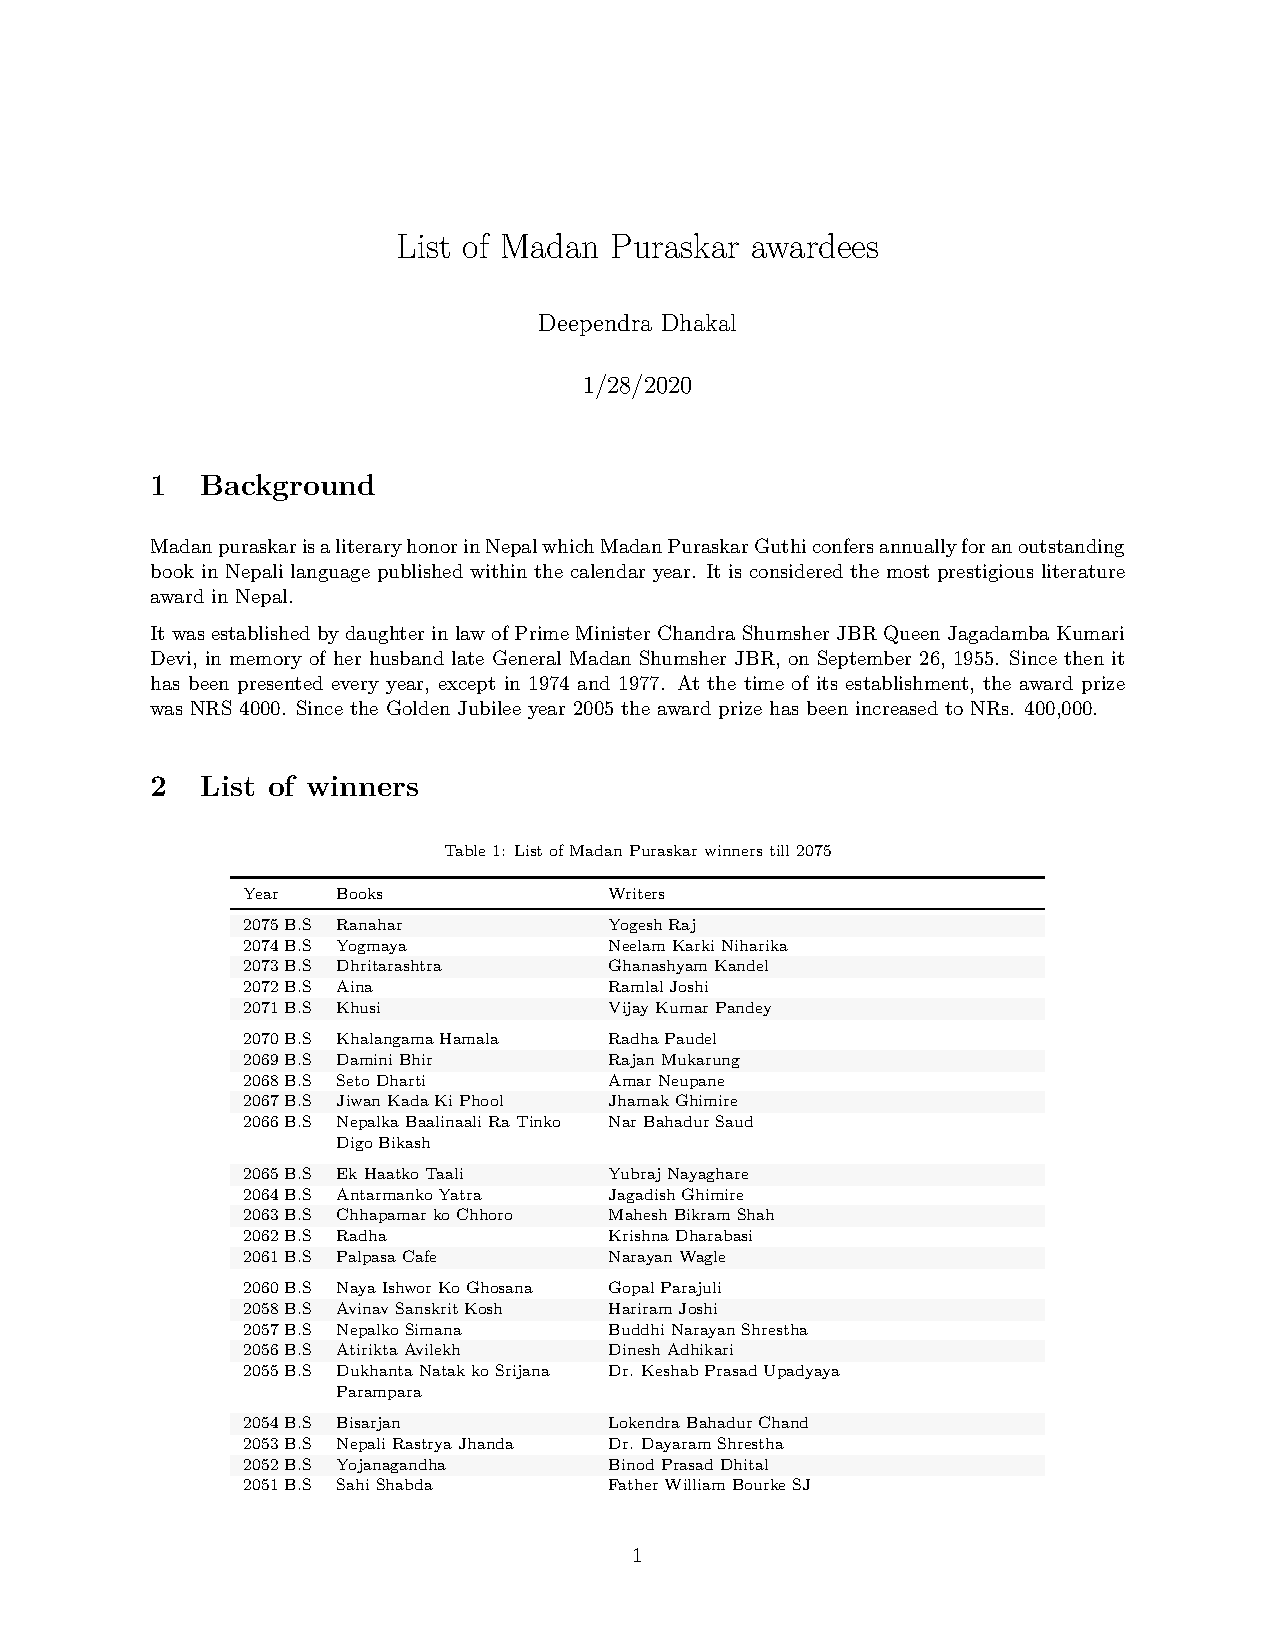
\includepdf[pages=-,pagecommand={},width=1.2\textwidth]{./latex_book/madan_puraskar_awardees.pdf}

  \bibliography{bibliography/vegetable.bib,bibliography/bib.bib}

\end{document}
